\documentclass[12pt]{article}

\usepackage[utf8]{inputenc}
\usepackage{tikz, url, hyperref, setspace, amsmath, amssymb, amsthm, graphicx, subcaption}
\usepackage[shortlabels]{enumitem}
\usepackage[ 
  backend = biber, 
  sorting = none, 
  style = numeric-comp,
]{biblatex}

\doublespacing

\addbibresource{refs.bib}
\tikzset{every picture/.style={line width=0.75pt}} %set default line width to 0.75pt        

\newcommand{\R}{\mathbb{R}}
\newcommand{\ci}{\perp\!\!\!\perp}
\newcommand{\KL}[1]{\operatorname{KL}\left[#1\right]}
\newcommand{\Ent}[1]{\operatorname{H}\left[#1\right]}
\newcommand{\CMI}[1]{\operatorname{I}\left[#1\right]}
\newcommand{\E}[2][{}]{\mathbb{E}_{#1}\left[#2\right]}
\newcommand{\Prob}[1]{\operatorname{P}\left(#1\right)}
\newcommand{\CM}[1]{\operatorname{CM}\left[#1\right]}
\newcommand{\floor}[1]{\left\lfloor #1 \right\rfloor}
\newcommand{\decimal}[1]{\left\{ #1 \right\}}
\newcommand{\toadd}[1]{\noindent\fbox{%
    \parbox{\textwidth}{%
        #1
    }%
}}

\newtheorem{thm}{Theorem}[section]
\newtheorem{lem}[thm]{Lemma}
\newtheorem{prop}[thm]{Proposition}
\newtheorem{cor}[thm]{Corollary}
\newtheorem{qn}[thm]{Question}

\theoremstyle{definition}
\newtheorem{dfn}[thm]{Definition}
\newtheorem{fw}[thm]{Framework}
\newtheorem{exl}[thm]{Example}

\newcounter{subexl}[thm]
\renewcommand{\thesubexl}{\theexl~(\alph{subexl})}
\newenvironment{subexl}{
    \refstepcounter{subexl}
    \bigskip
    \noindent
    \textbf{(\alph{subexl})~}%
}{}

\numberwithin{equation}{section}
\numberwithin{figure}{section}
\numberwithin{table}{section}

\title{When is invariant learning rational?}

\author{Abhimanyu Pallavi Sudhir}
\date{Supervisor: Jeroen Lamb}

\begin{document}

\maketitle

\begin{abstract}
    We observe that invariant learning is sometimes effective in a supervised learning context even when the ``nuisance factors'' truly provide information on the target variable, and find sufficient conditions, in terms of information theory, for this to occur. Our work is the preliminary set-up for a significant line of research that could be opened into invariant learning in tasks where there are direct correlations between nuisance factors and the target variable.
\end{abstract}

% \begin{abstract}
%     It has long been known that equivariant learning is closely related to causal learning, or can be understood in the language of causal models -- formally, equivariance is seen as independence between some random variables in a causal model. It is observed, however, that equivariant learning may still be effective in the absence of such independence, i.e. in the presence of ``confounding'' (correlations) between these variables. We study when this is the case, and ask whether equivariance will still be discovered by equivariance-detecting algorithms in the presence of such confounding.
% \end{abstract}

\tableofcontents

\pagebreak
\section{Introduction}
\label{sec:intro}

Invariant learning is a problem in machine learning, wherein one seeks to ensure the learned function (or distribution, etc.) is unaffected by some set of transformations of the input space. A simple example of such a set of transformations is the group of rigid transformations (rotations and translations) acting on an input space of images. 

There is a significant corpus of literature detailing algorithms for learning invariantly to such particular transformation groups -- the chief approaches among these are: 

\begin{itemize}
    \item \textbf{Manifestly invariant architectures}, i.e. that can only learn functions that are invariant to those transformations -- e.g. group-convolutional neural networks \cite{cohen2} (of which the familiar convolutional neural networks are a special case). A particularly significant result (from \cite{trivedi}) is that any neural network architecture that is manifestly invariant to a compact group of transformations is a group-convolutional neural network.
    \item \textbf{Data augmentation}, i.e. adding transformations of the data points to ``teach'' the algorithm that these transformed inputs must be assigned the same label -- see e.g. \cite{ilse, sxchen}.
\end{itemize}

We will highlight two specific line of research in the literature to motivate the problem we study in our project.

\begin{enumerate}
    \item \textbf{The pathological 6 and 9 problem} (mentioned in e.g. \cite{varma, ling}) -- If you apply a rotation-invariant classification algorithm to distinguishing ``6''s and ``9''s, it will perform rather poorly, as a rotated ``6'' \emph{is} in fact, very likely a ``9'', and should be read as such. \cite{benton} argues that the task can still be considered to be invariant, except to a different set (in particular a partial semigroup) of transformations including only rotations up to a certain angle; however, it remains true that naive rotation-invariant learning will not be effective for this task.
    \item \textbf{Fairness in machine learning} (reviewed in e.g. \cite{oatml}) -- Consider a practical machine learning application used by say, a moneylender, to assess the probability of a loan applicant defaulting based on various variables (income, credit rating, etc.) Writers of machine learning ethics often argue \cite{fair} that some factors (typically ``sensitive'' variables like race and religion) ought to not be considered when predicting the output variable, as they only affect the output variable ``through'' their relationship with other input variables -- and furthermore, that even if sensitive variables \emph{do} provide non-redundant information (information not contained in the other input variables) about the output variable, they should still not be considered, for ethical reasons.
\end{enumerate}

(In the latter problem, invariance is understood to mean ``ignoring some variable ($X_2$) in favour of another ($X_1$) while learning the target ($Y$)''. It might not immediately be clear how this is related to invariant learning as we introduced it -- this is the \emph{statistical} notion of invariance, which we will motivate later in this section, and formally define in Sec~\ref{sec:inv}, but it should be clear how this generalizes our earlier notion. The group orbits from before are our $X_1$, while $X_2$ determines the place of a data point on that orbit.)

In the first motivating problem, we ask: What property of the distribution (of hand-drawn digits) is it, mathematically, that tells us we should not expect invariant learning to be effective in this case? In the second problem, we ask: what can we say about the effectiveness of learning invariant to sensitive variables even when these variables provide non-redundant information about our output variable? Both problems have to do with the fundamental question, which we seek to approach in this project: 

\begin{qn}
    \label{qn:1}
    Under what circumstances will invariant learning (with respect to a particular set of transformations, group or otherwise) be effective or rational?
\end{qn}

The closest work to our own is \cite{sxchen}, which we shall now briefly review.

\cite{sxchen} specifically looks at the effectiveness of data augmentation based approaches to invariant learning. Let the data $\{x_i\}_{i=1}^n$ be sampled from a random vector $X$ taking values in some set $\mathcal{X}$; and let the task be to learn the distribution of $X$ within some class of models parameterized by the parameter $\theta$. Then whereas ordinary learning seeks to minimize $\sum_{i=1}^n{L(\theta, x_i)}$, the paper argues that augmented learning is equivalent to minimizing $\sum_{i=1}^n{\bar{L}(\theta, x_i)}$ where:

\begin{equation*}
    \bar{L}(\theta, x)=\int_{G}{L(\theta, gX)\,d\mathbb{Q}(g)}
\end{equation*}

And $G$ is a compact topological group acting on $X$, $\mathbb{Q}(g)$ the Haar measure on $G$ from which the augmentations are assumed to be sampled (we use the Haar measure because we want to think of the transformations as ``uniformly distributed'').

$\bar L(\theta, x)$ may then be viewed as the conditional expectation of $L(\theta, x)$ over the random variable $[x]$, the orbit of $x$ under $G$. It then follows from the Rao-Blackwell theorem that if $[X]$ is sufficient for $\theta$ (which occurs if $\forall g\in G, \, X =_d gX$ ($=_d$ indicating equality in distribution)), then $\bar{L}$ has the same mean, and lower variance than $L$. Thus if $\forall g\in G, \, X =_d gX$ (what they call ``exact invariance''), then invariant learning is effective. 

However, our work differs from \cite{sxchen} in several key ways:

\begin{enumerate}
    \item Their work only considers the effectiveness of data augmentation based approaches to learning; instead, we seek to abstract away the method by which invariance is achieved, and instead formulate Question~\ref{qn:1} more generally: when is it effective to use an invariant learning approach, at all?
    \item Our main result has to do with the case where exact invariance does \emph{not} hold. While they also generalize their result to the case of ``approximate invariance'' $\forall g\in G, \, X \approx_d gX$ ($\approx_d$ indicating approximate equality in distribution, defined formally in terms of the Wasserstein metric), this is quite different from the case of we consider, as we will see. 
    \item Their work does not readily generalize to supervised learning tasks -- whereas we only study supervised learning tasks.
    
    In fact, we make here a correction to a claim made on p. 7 of the paper, it is claimed that for supervised learning applications where we seek to infer the conditional distribution $\Prob{Y\mid X}$, we can ask for exact invariance of $(X, Y)$, i.e. $\forall g\in G, \, (X, Y) \approx_d g\cdot (X, Y)$, where the action of $g$ on $Y$ is trivial. They claim that this means ``the probability of an image being a bird is [...] the same as the probability for a rotated image''.
    
    However, this is not quite true -- exact invariance of $(X, Y)$ should actually be read as ``the probability of finding an image and it being a bird, is the same as finding a rotated image and that being a bird''. For example, if the rotated image is much less likely to be found in a real (non-augmented) dataset, then we don't have exact invariance of $(X, Y)$, however this should not affect our decision to use invariant learning to infer $\Prob{Y\mid X}$. 
    
    The result of \cite{sxchen} remains correct, as certainly exact invariance of $(X, Y)$ implies the effectiveness of invariant learning -- however, this condition is simply stronger than necessary for supervised learning tasks, and we will later formulate a more appropriate notion of ``exact invariance'' for conditional distributions in Sec~\ref{sec:main}.
\end{enumerate}

We will mention that the second motivation we presented -- fairness in machine learning -- suggests a fundamental link between this problem and \emph{causal modeling}. We will mathematically formulate causal modeling in Sec~\ref{sec:cause}, but for now we will say that the idea that $X_2$ provides only redundant information on $Y$ once given $X_1$ is fundamentally a statement of conditional independence: we say $Y$ and $X_2$ are conditionally independent given $X_1$, or $\Prob{Y\mid X_1, X_2}=\Prob{Y\mid X_1}$, or $Y\ci X_2\mid X_1$. As we will see, this is the same as saying that $Y$ and $X_2$, while \emph{correlated}, are not directly causally linked -- performing an intervention on $X_2$ (i.e. changing $X_2$ while leaving $X_1$ unchanged) will not change $Y$. 

(Therefore in some fundamental sense, invariant learning is about learning causations rather than mere correlations. One may say that invariant learning is to be performed in the \emph{anticausal direction}, i.e. to learn $Y$ from $X$ when $Y$ is believed to be a cause for $X$ rather than the other way around. This fact has been understood in the literature at least informally -- e.g. the standard Bible of causal inference \cite{elements} highlights that anticausal learning is performed when the mechanisms being learned are ``disentangled''. We will not dwell on this highly abstracted perspective on causal inference, but it serves to put our work in perspective, and to motivate the use of a statistical rather than deterministic definition of invariance.)

Certainly invariant learning -- informally for our purposes, ignoring some variable $X_2$ while learning $\Prob{Y\mid X_1, X_2}$ -- is effective when $X_2$ is redundant for $Y$ given $X$, i.e. when $Y\ci X_2\mid X_1$. However, we often see that invariant learning is sometimes still effective even when this is \emph{not} the case.

\begin{figure}
    \centering
    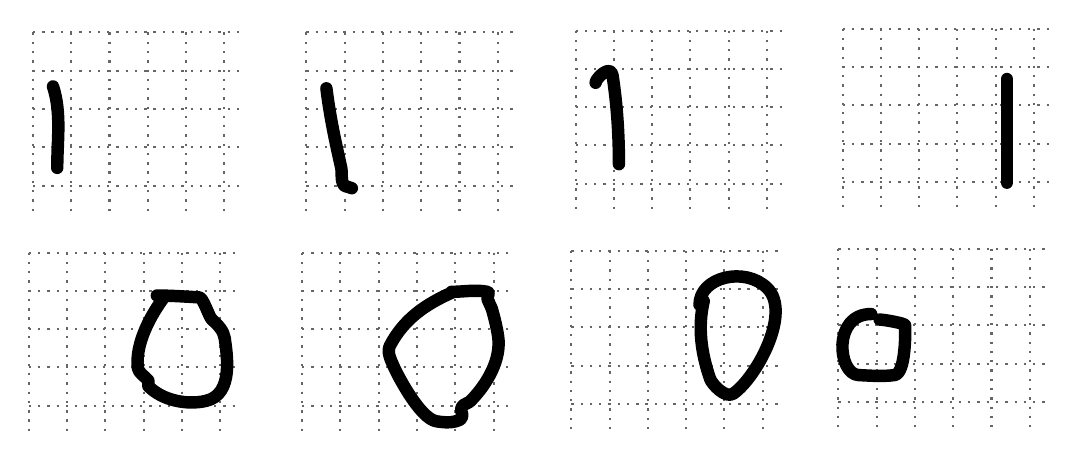
\begin{tikzpicture}[x=0.75pt,y=0.75pt,yscale=-1.5,xscale=1.5]
%uncomment if require: \path (0,479); %set diagram left start at 0, and has height of 479

%Shape: Grid [id:dp8017742479015741] 
\draw  [draw opacity=0][dash pattern={on 0.84pt off 2.51pt}] (86.7,177) -- (153.73,177) -- (153.73,234.28) -- (86.7,234.28) -- cycle ; \draw  [color={rgb, 255:red, 103; green, 101; blue, 101 }  ,draw opacity=1 ][dash pattern={on 0.84pt off 2.51pt}] (86.7,177) -- (86.7,234.28)(98.99,177) -- (98.99,234.28)(111.29,177) -- (111.29,234.28)(123.59,177) -- (123.59,234.28)(135.88,177) -- (135.88,234.28)(148.18,177) -- (148.18,234.28) ; \draw  [color={rgb, 255:red, 103; green, 101; blue, 101 }  ,draw opacity=1 ][dash pattern={on 0.84pt off 2.51pt}] (86.7,177) -- (153.73,177)(86.7,189.3) -- (153.73,189.3)(86.7,201.59) -- (153.73,201.59)(86.7,213.89) -- (153.73,213.89)(86.7,226.19) -- (153.73,226.19) ; \draw  [color={rgb, 255:red, 103; green, 101; blue, 101 }  ,draw opacity=1 ][dash pattern={on 0.84pt off 2.51pt}]  ;
%Shape: Free Drawing [id:dp8064467449652992] 
\draw  [line width=4.5] [line join = round][line cap = round] (93.14,194.35) .. controls (95.89,202.74) and (94.5,211.78) .. (94.5,220.5) ;
%Shape: Grid [id:dp7763004534165105] 
\draw  [draw opacity=0][dash pattern={on 0.84pt off 2.51pt}] (174.52,177) -- (241.56,177) -- (241.56,234.28) -- (174.52,234.28) -- cycle ; \draw  [color={rgb, 255:red, 103; green, 101; blue, 101 }  ,draw opacity=1 ][dash pattern={on 0.84pt off 2.51pt}] (174.52,177) -- (174.52,234.28)(186.82,177) -- (186.82,234.28)(199.11,177) -- (199.11,234.28)(211.41,177) -- (211.41,234.28)(223.71,177) -- (223.71,234.28)(236,177) -- (236,234.28) ; \draw  [color={rgb, 255:red, 103; green, 101; blue, 101 }  ,draw opacity=1 ][dash pattern={on 0.84pt off 2.51pt}] (174.52,177) -- (241.56,177)(174.52,189.3) -- (241.56,189.3)(174.52,201.59) -- (241.56,201.59)(174.52,213.89) -- (241.56,213.89)(174.52,226.19) -- (241.56,226.19) ; \draw  [color={rgb, 255:red, 103; green, 101; blue, 101 }  ,draw opacity=1 ][dash pattern={on 0.84pt off 2.51pt}]  ;
%Shape: Free Drawing [id:dp7728025162953451] 
\draw  [line width=4.5] [line join = round][line cap = round] (180.96,194.95) .. controls (182.01,203.62) and (183.82,212.14) .. (185.73,220.5) .. controls (186.13,222.26) and (185.49,224.25) .. (186.41,225.85) .. controls (187.02,226.91) and (188.2,226.22) .. (189.13,227.04) ;
%Shape: Grid [id:dp29771297583850953] 
\draw  [draw opacity=0][dash pattern={on 0.84pt off 2.51pt}] (260.98,176.41) -- (328.02,176.41) -- (328.02,233.69) -- (260.98,233.69) -- cycle ; \draw  [color={rgb, 255:red, 103; green, 101; blue, 101 }  ,draw opacity=1 ][dash pattern={on 0.84pt off 2.51pt}] (260.98,176.41) -- (260.98,233.69)(273.28,176.41) -- (273.28,233.69)(285.58,176.41) -- (285.58,233.69)(297.87,176.41) -- (297.87,233.69)(310.17,176.41) -- (310.17,233.69)(322.47,176.41) -- (322.47,233.69) ; \draw  [color={rgb, 255:red, 103; green, 101; blue, 101 }  ,draw opacity=1 ][dash pattern={on 0.84pt off 2.51pt}] (260.98,176.41) -- (328.02,176.41)(260.98,188.7) -- (328.02,188.7)(260.98,201) -- (328.02,201)(260.98,213.3) -- (328.02,213.3)(260.98,225.59) -- (328.02,225.59) ; \draw  [color={rgb, 255:red, 103; green, 101; blue, 101 }  ,draw opacity=1 ][dash pattern={on 0.84pt off 2.51pt}]  ;
%Shape: Free Drawing [id:dp08059093421743646] 
\draw  [line width=4.5] [line join = round][line cap = round] (267.43,193.17) .. controls (267.43,191.71) and (272.31,187.08) .. (272.87,190.79) .. controls (274.32,200.23) and (274.92,209.79) .. (274.92,219.31) ;
%Shape: Grid [id:dp45413993373677175] 
\draw  [draw opacity=0][dash pattern={on 0.84pt off 2.51pt}] (346.77,175.81) -- (413.8,175.81) -- (413.8,233.09) -- (346.77,233.09) -- cycle ; \draw  [color={rgb, 255:red, 103; green, 101; blue, 101 }  ,draw opacity=1 ][dash pattern={on 0.84pt off 2.51pt}] (346.77,175.81) -- (346.77,233.09)(359.06,175.81) -- (359.06,233.09)(371.36,175.81) -- (371.36,233.09)(383.65,175.81) -- (383.65,233.09)(395.95,175.81) -- (395.95,233.09)(408.25,175.81) -- (408.25,233.09) ; \draw  [color={rgb, 255:red, 103; green, 101; blue, 101 }  ,draw opacity=1 ][dash pattern={on 0.84pt off 2.51pt}] (346.77,175.81) -- (413.8,175.81)(346.77,188.11) -- (413.8,188.11)(346.77,200.41) -- (413.8,200.41)(346.77,212.7) -- (413.8,212.7)(346.77,225) -- (413.8,225) ; \draw  [color={rgb, 255:red, 103; green, 101; blue, 101 }  ,draw opacity=1 ][dash pattern={on 0.84pt off 2.51pt}]  ;
%Shape: Free Drawing [id:dp7154116232984749] 
\draw  [line width=4.5] [line join = round][line cap = round] (399.5,191.98) .. controls (399.5,203.07) and (399.5,214.16) .. (399.5,225.26) ;
%Shape: Grid [id:dp2704962527573529] 
\draw  [draw opacity=0][dash pattern={on 0.84pt off 2.51pt}] (85.34,247.72) -- (152.37,247.72) -- (152.37,305) -- (85.34,305) -- cycle ; \draw  [color={rgb, 255:red, 103; green, 101; blue, 101 }  ,draw opacity=1 ][dash pattern={on 0.84pt off 2.51pt}] (85.34,247.72) -- (85.34,305)(97.63,247.72) -- (97.63,305)(109.93,247.72) -- (109.93,305)(122.23,247.72) -- (122.23,305)(134.52,247.72) -- (134.52,305)(146.82,247.72) -- (146.82,305) ; \draw  [color={rgb, 255:red, 103; green, 101; blue, 101 }  ,draw opacity=1 ][dash pattern={on 0.84pt off 2.51pt}] (85.34,247.72) -- (152.37,247.72)(85.34,260.02) -- (152.37,260.02)(85.34,272.31) -- (152.37,272.31)(85.34,284.61) -- (152.37,284.61)(85.34,296.9) -- (152.37,296.9) ; \draw  [color={rgb, 255:red, 103; green, 101; blue, 101 }  ,draw opacity=1 ][dash pattern={on 0.84pt off 2.51pt}]  ;
%Shape: Grid [id:dp20012418254236608] 
\draw  [draw opacity=0][dash pattern={on 0.84pt off 2.51pt}] (173.16,247.72) -- (240.19,247.72) -- (240.19,305) -- (173.16,305) -- cycle ; \draw  [color={rgb, 255:red, 103; green, 101; blue, 101 }  ,draw opacity=1 ][dash pattern={on 0.84pt off 2.51pt}] (173.16,247.72) -- (173.16,305)(185.46,247.72) -- (185.46,305)(197.75,247.72) -- (197.75,305)(210.05,247.72) -- (210.05,305)(222.35,247.72) -- (222.35,305)(234.64,247.72) -- (234.64,305) ; \draw  [color={rgb, 255:red, 103; green, 101; blue, 101 }  ,draw opacity=1 ][dash pattern={on 0.84pt off 2.51pt}] (173.16,247.72) -- (240.19,247.72)(173.16,260.02) -- (240.19,260.02)(173.16,272.31) -- (240.19,272.31)(173.16,284.61) -- (240.19,284.61)(173.16,296.9) -- (240.19,296.9) ; \draw  [color={rgb, 255:red, 103; green, 101; blue, 101 }  ,draw opacity=1 ][dash pattern={on 0.84pt off 2.51pt}]  ;
%Shape: Grid [id:dp9881793507958303] 
\draw  [draw opacity=0][dash pattern={on 0.84pt off 2.51pt}] (259.62,247.12) -- (326.66,247.12) -- (326.66,304.41) -- (259.62,304.41) -- cycle ; \draw  [color={rgb, 255:red, 103; green, 101; blue, 101 }  ,draw opacity=1 ][dash pattern={on 0.84pt off 2.51pt}] (259.62,247.12) -- (259.62,304.41)(271.92,247.12) -- (271.92,304.41)(284.22,247.12) -- (284.22,304.41)(296.51,247.12) -- (296.51,304.41)(308.81,247.12) -- (308.81,304.41)(321.1,247.12) -- (321.1,304.41) ; \draw  [color={rgb, 255:red, 103; green, 101; blue, 101 }  ,draw opacity=1 ][dash pattern={on 0.84pt off 2.51pt}] (259.62,247.12) -- (326.66,247.12)(259.62,259.42) -- (326.66,259.42)(259.62,271.72) -- (326.66,271.72)(259.62,284.01) -- (326.66,284.01)(259.62,296.31) -- (326.66,296.31) ; \draw  [color={rgb, 255:red, 103; green, 101; blue, 101 }  ,draw opacity=1 ][dash pattern={on 0.84pt off 2.51pt}]  ;
%Shape: Grid [id:dp5786980285185035] 
\draw  [draw opacity=0][dash pattern={on 0.84pt off 2.51pt}] (345.4,246.53) -- (412.44,246.53) -- (412.44,303.81) -- (345.4,303.81) -- cycle ; \draw  [color={rgb, 255:red, 103; green, 101; blue, 101 }  ,draw opacity=1 ][dash pattern={on 0.84pt off 2.51pt}] (345.4,246.53) -- (345.4,303.81)(357.7,246.53) -- (357.7,303.81)(370,246.53) -- (370,303.81)(382.29,246.53) -- (382.29,303.81)(394.59,246.53) -- (394.59,303.81)(406.89,246.53) -- (406.89,303.81) ; \draw  [color={rgb, 255:red, 103; green, 101; blue, 101 }  ,draw opacity=1 ][dash pattern={on 0.84pt off 2.51pt}] (345.4,246.53) -- (412.44,246.53)(345.4,258.83) -- (412.44,258.83)(345.4,271.12) -- (412.44,271.12)(345.4,283.42) -- (412.44,283.42)(345.4,295.72) -- (412.44,295.72) ; \draw  [color={rgb, 255:red, 103; green, 101; blue, 101 }  ,draw opacity=1 ][dash pattern={on 0.84pt off 2.51pt}]  ;
%Shape: Free Drawing [id:dp07051563274345996] 
\draw  [line width=4.5] [line join = round][line cap = round] (129.22,261.51) .. controls (124.41,267.81) and (119.57,276.93) .. (120.37,284.68) .. controls (120.55,286.38) and (122.69,287.43) .. (123.78,288.84) .. controls (124.15,289.34) and (123.33,290.17) .. (123.78,290.63) .. controls (128.16,295.09) and (135.81,296.77) .. (142.16,295.38) .. controls (151.5,293.34) and (148.86,279.69) .. (148.29,275.18) .. controls (147.99,272.88) and (146.07,270.87) .. (144.2,269.23) .. controls (143.25,268.4) and (141.4,262.17) .. (140.12,262.1) .. controls (135.58,261.85) and (131.04,261.51) .. (126.5,261.51) ;
%Shape: Free Drawing [id:dp20550417919662056] 
\draw  [line width=4.5] [line join = round][line cap = round] (221.81,260.32) .. controls (212.92,264.2) and (205.93,268.96) .. (201.39,277.55) .. controls (200.23,279.74) and (201.79,282.42) .. (202.75,284.68) .. controls (203.32,286.02) and (210.86,301.12) .. (216.37,301.92) .. controls (218.38,302.21) and (220.56,302.48) .. (222.49,301.92) .. controls (226.66,300.71) and (223.27,299.09) .. (224.54,297.16) .. controls (225.1,296.3) and (226.52,296.13) .. (227.26,295.38) .. controls (232.62,289.92) and (237.22,281.99) .. (236.11,274.58) .. controls (235.66,271.58) and (234.91,268.61) .. (234.07,265.67) .. controls (233.77,264.63) and (232.97,263.74) .. (232.71,262.7) .. controls (232.51,261.92) and (233.59,260.5) .. (232.71,260.32) .. controls (228.95,259.55) and (224.99,260.32) .. (221.13,260.32) ;
%Shape: Free Drawing [id:dp981270324750338] 
\draw  [line width=4.5] [line join = round][line cap = round] (302.15,263.29) .. controls (300.22,271.72) and (301.32,279.89) .. (304.19,288.25) .. controls (304.77,289.93) and (309.16,294.76) .. (311.68,293) .. controls (319.13,287.8) and (330.45,266.92) .. (322.57,259.13) .. controls (315.4,252.04) and (300.79,255.57) .. (300.79,264.48) ;
%Shape: Free Drawing [id:dp5609590941584457] 
\draw  [line width=4.5] [line join = round][line cap = round] (355.93,267.45) .. controls (343.39,267.45) and (345.26,286.76) .. (351.85,287.06) .. controls (355.7,287.24) and (359.61,287.56) .. (363.42,287.06) .. controls (367.17,286.57) and (366.94,272.33) .. (366.82,271.02) .. controls (366.77,270.42) and (359.88,269.23) .. (358.65,269.23) ;




\end{tikzpicture}

    \caption{The target variable, the label, is directly correlated with the nuisance variable, the position of the image. }
    \label{fig:real-sample-0}
\end{figure}

In Fig~\ref{fig:real-sample-0}, even though $X_2$ provides significant information on $Y$, we may still ignore it, because $X_1$ alone is also sufficient to determine $Y$ with a great degree of accuracy. However, if we were classifying ``6''s and ``9''s, the orbit of a character under rotation would \emph{not} carry sufficient information about $Y$ -- indeed, the orbit of a ``6'' image could indicate either a ``6'' or a ``9'', so ignoring the rotation and relying only on the orbit in learning the label would not be effective. 

This very intuitive result is, in a nutshell, what we will aim to formally explain in this project.

An immediate implication of our result will be to fairness in machine learning -- it will bound the error when applying ``fair'' (invariant) algorithms even when sensitive variables provide non-redundant information. For this reason and others, we suggest that further theoretical study of invariant learning in situations with non-redundant information will be valuable, and outline directions for future research in this area.

% Furthermore, there are algorithms that discover invariances in a dataset -- e.g. Augerino \cite{benton}, which parameterizes a distribution of transformations with a neural network and trains it. We may correspondingly ask:

% \begin{qn}
%     \label{qn:2}
%     Will invariance discovery algorithms (like Augerino) discover invariances whenever it is effective to learn invariantly to those transformations?
% \end{qn}

\subsection{Notation and conventions}

Below is a list of notation we will use throughout this report without definition:

\begin{itemize}
    \item \emph{Probability theory} -- Let $\Omega$ be a sample space, let $\mathcal{A}_i,\mathcal{B}_j, \mathcal{C}$ ($1\le i\le m$, $1\le j\le n$) be measure spaces: in particular, each $\mathcal{A}_i$ is a countable set with the counting measure $\alpha_i$, and each $\mathcal{B}_j$ is a copy of $\mathcal{R}^{n_j}$ with the Lesbesgue measure $\beta_j$.
    \begin{itemize}
        \item A measurable function $\Omega\to \mathcal{C}$ is called a ``random quantity on $\mathcal{C}$''. Hereon, we will omit mentioning the sample space $\Omega$ and assume that all random quantities are defined on the same sample space.
        \item $\Prob{A_1,\dots A_n, B_1, \dots B_n}$ denotes, for $A_i, B_j$ random quantities on $\mathcal{A}_i,\mathcal{B}_j$ respectively, the probability density function with respect to $\alpha_1\otimes\dots\otimes\alpha_m\otimes\beta_1\otimes\dots\otimes\beta_n$. Analogously for conditional probabilities.
        \item $\E{\dots}$ is the expectation. If the term within the parentheses is a function of some random quantities $f(C_1,\dots C_k)$, we may write the expectation as $\E[c_1,\dots c_k\sim C_1,\dots C_k]{f(c_1,\dots c_k)}$.  Analogously for conditional expectation with respect to a random variable, we write $\E[c_1,\dots c_k\mid c_{k+1}\dots c_l \sim C_1,\dots C_k\mid C_{k+1}\dots C_l]{f(c_1,\dots c_k)\mid C_{k+1}=c_{k+1}\dots C_l=c_l} = \int{f(c_1,\dots c_k)\,d(\gamma_1\otimes\dots\otimes\gamma_k\mid\gamma_{k+1}\otimes\dots\otimes\gamma_{k})}$ where $\gamma_i$ denote the probability measures on the respective sets in which $C_i$ take values, and $\mu\mid\nu$ denotes the regular conditional probability measure of $\mu$ against $\nu$.
        \item The notation $A\ci B$ represents independence, and is to be read $A$ and $B$ are independent, i.e. $\Prob{A\mid B}=\Prob{A}$; $A\ci B\mid C$ represents conditional independence, and is to be read ``$A$ and $B$ are independent, conditional on $C$'', i.e. $\Prob{A\mid B, C}=\Prob{A\mid C}$. 
        \item The notation $=_d$ reads ``equal in distribution to'', and the notation $\approx_d$ reads ``approximately equal in distribution to''.
    \end{itemize}
    \item \emph{Graph theory} -- Let $\mathbf{V}$ be a graph consisting of vertices labelled $V_1,\dots V_n$. 
    \begin{itemize}
        \item $\mathrm{Parents}(V_i)$ is the set of parents of $V_i$ in the graph $\mathbf{V}$, i.e. of the nodes $V_k$ with an arrow going $V_k\to V_i$.
        \item $\mathrm{Descendants}(V_i)$ is the set of descendants of $V_i$ in the graph $\mathbf{V}$, i.e. of the nodes $V_k$ such that there exists some ordered list $(V_{i_1}, V_{i_2}, \dots V_{i_m})$ ($m\ge 1$) where $V_{i_1}=V_i$, $V_{i_m}=V_k$ and $\forall j<m$ there is an edge directed $V_{i_j}\rightarrow V_{i_{j+1}}$. Note that in particular $V_i\in\mathrm{Descendants}(V_i)$.
    \end{itemize}
    \item \emph{Information theory} -- We use the standard notations for entropies; three particular entropies that will be of relevance to us are listed below. All logarithms are base 2 unless stated otherwise.
    \begin{itemize}
        \item Let $p$ and $q$ be distributions on some discrete space $\mathcal{B}$ -- then $\Ent{p,q}:=-\sum_{b\in\mathcal{B}}{p(b)\log q(b)}$ denotes the cross-entropy of the distributions. 
        \item Let $A$ and $B$ be random quantities on measurable spaces $\mathcal{A}$, $\mathcal{B}$ respectively; then $\Ent{B\mid A}:=-\E[a,b\sim A, B]{\log \Prob{b\mid a}}$ denotes the conditional entropy of $B$ given $A$.
    \end{itemize}
\end{itemize}

\pagebreak
\section{Prerequisites and literature} 

\subsection{Invariance}
\label{sec:inv}

We will detail a sequence of definitions of invariance from the literature, short of the generalized definitions we will give in Secs~\ref{sec:q},~\ref{sec:main}. 

Def~\ref{dfn:inv-det-group} gives the ``canonical'' or most basic definitions of equivariance and invariance, as used in \cite{trivedi} (similar definitions are assumed in \cite{cohen, cohen2, esteves, gerken, reiset}).

\begin{dfn}[Invariance -- deterministic; group]
    \label{dfn:inv-det-group}
    Where $G$ is a group acting on $\mathcal{X}$ and $\mathcal{Y}$, a function $f:\mathcal{X}\to \mathcal{Y}$ is said to be $G$-equivariant if $\forall g\in G$ and $\forall x\in \mathcal{X}$: 
    \begin{equation*}
        f(g(x))=g(f(x))
    \end{equation*}
    Of particular interest is the case where the action of $G$ on $\mathcal{Y}$ is $\mathrm{id}$ -- $f$ is said to be $G$-invariant if $\forall g\in G$ and $\forall x\in \mathcal{X}$: 
    \begin{equation*}
        f(g(x))=f(x)
    \end{equation*}
\end{dfn}

Def~\ref{dfn:inv-det-part} generalizes Def~\ref{dfn:inv-det-group} to any partition on $\mathcal{X}$, not just the quotient space of the group action, $\mathcal{X}/G$. We mention this generalization, as this will closely connect to our later definitions of invariance. 

\begin{dfn}[Invariance -- deterministic; partition]
    \label{dfn:inv-det-part}
    Where $R$ is an equivalence relation on $\mathcal{X}$, a function $f:\mathcal{X}\to \mathcal{Y}$ is said to be $R$-invariant if it is a function purely on the partition defined by $R$, i.e. $\forall x,x'\in \mathcal{X}$: 
    \begin{equation*}
        [x]_R=[x']_R \implies f(x)=f(x')
    \end{equation*}
\end{dfn}

These definitions so far have been for a \emph{deterministic function} $f$. In this project, we will instead treat learning as a statistical inference problem, i.e. of inferring the distribution $\Prob{Y\mid X}$ from data. We will state two statistical formulations of invariance and discuss their relevance (or lack thereof) to our problem, so as to better justify the definition we will make in Sec~\ref{sec:q}.

\begin{dfn}[Invariance -- definition in \cite{achille}]
    \label{dfn:inv-stat-achille}
    Let $\mathcal{X},\mathcal{Y}$ be sets ($\mathcal{Y}$ discrete), and $X, Y$ are random quantities taking values in $\mathcal{X},\mathcal{Y}$ (i.e. they are measurable functions $\Omega\to \mathcal{X}$, $\Omega\to \mathcal{Y}$ for sample space $\Omega$). Now let:
    \begin{itemize}
        \item $T$ be a \emph{representation} of $X$: a random quantity on a set $\mathcal{T}$ such that $T\ci Y\mid X$.
        \item $N$ be a \emph{nuisance} to $Y$: a random quantity on a set $\mathcal{N}$ such that $Y\ci N$. 
    \end{itemize}
    Then $T$ is said to be an $N$-invariant representation if $T\ci N$. 
\end{dfn}

Def~\ref{dfn:inv-stat-achille} is the formulation of invariance in Def~\cite{achille} -- it defines what it means for a representation (given by a random variable of its own) to be invariant to some nuisance variable. 

This definition is somewhat hard to motivate, because the goal of \cite{achille} is different from ours -- it is to give an explanation for the effectiveness of deep neural networks, arguing that this has to do with a certain propensity for deep neural networks to learn invariant representations when the number of hidden layers is large. In particular, it has a crucial limitation for our purposes: it \emph{presumes}, a priori, that $Y\ci N$ -- whereas our central result Thm~\ref{thm:main} says essentially that invariant learning is rational when $Y\ci N$, and that it can still be rational otherwise under certain conditions. 

\begin{dfn}[Invariance -- definition in \cite{sxchen}]
    \label{dfn:inv-stat-sxchen}
    Let $\mathcal{Z}$ be a set, $Z$ be a random quantity taking values in $\mathcal{Z}$, and $G$ be a group acting on $\mathcal{Z}$. Then $Z$ is said to be $G$-invariant if  for any $g\in G$, $gZ =_d Z$ (i.e. $gZ$ has the same distribution as $Z$).
\end{dfn}

Def~\ref{dfn:inv-stat-sxchen} is the formulation of invariance in Def~\cite{sxchen} -- it defines what it means for a distribution to be invariant. This is a fundamentally different idea than invariant representations -- we're no longer talking about the invariance of an inferred distribution, but of the ``true'' distribution of the data. One may imagine that the relationship is closely relevant to Question~\ref{qn:1} -- indeed, if the ``true'' distribution is invariant (and we will there define this in a slightly more general way than below), then it is effective to learn invariantly. 

\subsection{Causation}
\label{sec:cause}

As discussed in Sec~\ref{sec:intro}, there is a close relationship between invariance and causal modeling. We will formally introduce causal modeling in this section; however, as causation is not the primary topic of this project, we will not dwell too long explaining the definitions, nor will we provide proofs for the propositions -- full treatments can be found in \cite{pearl, elements}.

At first, causation might seem like something outside the domain of serious statistics -- indeed, for a long period of history, statisticians believed that causation could not be determined without knowing timestamps, or without performing direct interventions. However, this is no longer the case -- indeed, causation must be a physically valid concept, because it is testable: for example, in Fig~\ref{fig:causation-distinct}: ``rain causes wet grass'' can be distinguished from ``wet grass causes rain'' by turning on the sprinkler and checking if this results in rain. 

\begin{figure}
    \centering
    \input{causation-distinct.tex}
    \caption{Distinct causal models}
    \label{fig:causation-distinct}
\end{figure}

\begin{figure}
    \centering
    \begin{tikzpicture}[x=0.75pt,y=0.75pt,yscale=-1.5,xscale=1.5]
%uncomment if require: \path (0,235); %set diagram left start at 0, and has height of 235

%Straight Lines [id:da9173659620649355] 
\draw    (150.87,83.69) -- (196.8,156.01) ;
\draw [shift={(149.8,82)}, rotate = 57.58] [color={rgb, 255:red, 0; green, 0; blue, 0 }  ][line width=0.75]    (10.93,-3.29) .. controls (6.95,-1.4) and (3.31,-0.3) .. (0,0) .. controls (3.31,0.3) and (6.95,1.4) .. (10.93,3.29)   ;
%Straight Lines [id:da683079525010619] 
\draw    (267.77,82.51) -- (223.8,155.8) ;
\draw [shift={(268.8,80.8)}, rotate = 120.96] [color={rgb, 255:red, 0; green, 0; blue, 0 }  ][line width=0.75]    (10.93,-3.29) .. controls (6.95,-1.4) and (3.31,-0.3) .. (0,0) .. controls (3.31,0.3) and (6.95,1.4) .. (10.93,3.29)   ;
%Straight Lines [id:da49180269404387955] 
\draw    (372.8,125.01) -- (372.8,161.01) ;
\draw [shift={(372.8,163.01)}, rotate = 270] [color={rgb, 255:red, 0; green, 0; blue, 0 }  ][line width=0.75]    (10.93,-3.29) .. controls (6.95,-1.4) and (3.31,-0.3) .. (0,0) .. controls (3.31,0.3) and (6.95,1.4) .. (10.93,3.29)   ;
%Straight Lines [id:da26506430315689467] 
\draw    (372.8,66.01) -- (372.8,98.01) ;
\draw [shift={(372.8,100.01)}, rotate = 270] [color={rgb, 255:red, 0; green, 0; blue, 0 }  ][line width=0.75]    (10.93,-3.29) .. controls (6.95,-1.4) and (3.31,-0.3) .. (0,0) .. controls (3.31,0.3) and (6.95,1.4) .. (10.93,3.29)   ;

% Text Node
\draw (133,57.19) node [anchor=north west][inner sep=0.75pt]   [align=left] {rain};
% Text Node
\draw (241,57.19) node [anchor=north west][inner sep=0.75pt]   [align=left] {sprinkler};
% Text Node
\draw (173.8,163) node [anchor=north west][inner sep=0.75pt]   [align=left] {wet grass};
% Text Node
\draw (342,102.19) node [anchor=north west][inner sep=0.75pt]   [align=left] {wet grass};
% Text Node
\draw (346,44.19) node [anchor=north west][inner sep=0.75pt]   [align=left] {sprinkler};
% Text Node
\draw (359.8,170) node [anchor=north west][inner sep=0.75pt]   [align=left] {rain};


\end{tikzpicture}

    \caption{Equivalent causal models}
    \label{fig:causation-identical}
\end{figure}

We will shortly define formally what these arrows mean; but intuitively, a statement of causation can fundamentally only be expressed \emph{relative} to some set of ``control variables'', namely in terms of independences conditional on these control variables. 

\begin{dfn}[Causal model]
    \label{dfn:causation}
    Let the random variables $X_1,\dots X_n$ be sampled from some joint distribution $\Prob{X_1,\dots,X_n}$. Have $\mathbf{X}$ be a Directed Acyclic Graph (DAG) of $X_1,\dots X_n$ (i.e. with these random variables uniquely represented as its nodes); then the ordered list $$(\mathbf{X}, \Prob{X_1\mid\mathrm{Parents}(X_1)}, \dots, \Prob{X_n\mid\mathrm{Parents}(X_n))}$$ is called a causal model for $\Prob{X_1,\dots X_n}$.
\end{dfn}

Def~\ref{dfn:causation} alone makes no non-trivial statement about the joint distribution $\Prob{X_1,\dots,X_n}$ -- indeed, any such causal model could be constructed for any joint distribution. What gives meaning to a causal model is the \emph{Causal Markov condition} (Def~\ref{dfn:causation-markov}), or equivalently Markov factorization (Prop~\ref{prop:causation-mf}), or equivalently $d$-Separation (Prop~\ref{prop:causation-dsep}). 

Briefly: the Causal Markov condition states that a causal model implies certain conditional independencies, the ``hypothesis'' entailed by the model; Markov factorization makes this hypothesis algebraically explicit -- as the statement that specifying certain conditional distributions suffices to determine the joint distribution; $d$-Separation provides a rather intuitive picture for conditional independence as the absence of ``unblocked paths'' between two nodes for information to flow through.

\begin{dfn}[Causal Markov condition]
    \label{dfn:causation-markov}
    A causal model as in Def~\ref{dfn:causation} is said to be \emph{causally Markov} if $\forall X\in\mathbf{X}, X\ci \mathrm{Descendants}(X)^{\mathrm{C}}\mid\mathrm{Parents}(X)$
\end{dfn}

\begin{prop}[Markov factorization]
    \label{prop:causation-mf}
    A causal model as in Def~\ref{dfn:causation} is causally Markov if and only if:
    \begin{equation*}
        \Prob{X_1,\dots,X_n} = \prod_i \Prob{X_i\mid \mathrm{Parents}(X_i)}
    \end{equation*}
\end{prop}

\begin{dfn}[$d$-Separation]
    \label{dfn:causation-dsep}
    In any DAG $\mathbf{X}$, an ordered list of nodes $(X_{i_1}, \dots X_{i_m})$ such that for all $j$, there is either an edge directed $X_{i_j}\rightarrow X_{i_{j+1}}$ or an edge directed $X_{i_j}\leftarrow X_{i_{j+1}}$ -- is called a \emph{path} and is denoted as $X_{i_1}\to X_{i_2} \leftarrow \dots \leftarrow X_{i_m}$ depending on which edge exists between each consecutive pair of nodes. Each node $X_{i_2},\dots X_{i_{m-1}}$ is called a ``junction'' -- a node $X_{i_j}$ is classified into one of three types, as follows:
    \begin{itemize}
        \item ``Chain'' if there are edges directed $X_{i_{j-1}}\rightarrow X_{i_{j}}\rightarrow X_{i_{j+1}}$
        \item ``Fork'' if there are edges directed $X_{i_{j-1}}\leftarrow X_{i_{j}}\rightarrow X_{i_{j+1}}$
        \item ``Collider'' if there are edges directed $X_{i_{j-1}}\rightarrow X_{i_{j}}\leftarrow X_{i_{j+1}}$
    \end{itemize}
    Let $\mathbf{Y}\subseteq \mathbf{X}$. Then we say a junction $X_{i_j}$ is ``blocked when conditioned on $\mathbf{Y}$'' iff one of the following holds (and unblocked ditto otherwise):
    \begin{itemize}
        \item It is a chain junction, and $\mathrm{Descendants}(X_{i_j})\cap\mathbf{Y}\ne\varnothing$.
        \item It is a fork junction, and $\mathrm{Descendants}(X_{i_j})\cap\mathbf{Y}\ne\varnothing$.
        \item It is a collider junction, and $\mathrm{Descendants}(X_{i_j})\cap\mathbf{Y}=\varnothing$.
    \end{itemize}
    The ordered list $(X_{i_1}, \dots X_{i_m})$ is said to be ``blocked when conditioned on $\mathbf{Y}$'' iff any one of its junctions $X_{i_2},\dots X_{i_{m-1}}$ is blocked when conditioned on $\mathbf{Y}$. 
    
    Two nodes $X_{1}$ and $X_{2}$ are said to be ``$d$-separated when conditioned on $\mathbf{Y}$'' ($X_1\nleftrightarrow X_2 \mid\mathbf{Y}$) if all paths between them are blocked when conditioned on $\mathbf{Y}$.
    
    Two subsets $\mathbf{X}_1,\mathbf{X}_2\subseteq\mathbf{X}$ are said to be ``$d$-separated when conditioned on $\mathbf{Y}$'' ($\mathbf{X}_1\nleftrightarrow\mathbf{X}_2\mid\mathbf{Y}$) if each pair $X_1\in\mathbf{X}_1$, $X_2\in\mathbf{X}_2$ are $d$-separated when conditioned on $\mathbf{Y}$.
\end{dfn}

\begin{prop}[$d$-Separation]
    \label{prop:causation-dsep}
    A causal model as in Def~\ref{dfn:causation} is causally Markov if and only if $\forall\mathbf{X}_1,\mathbf{X}_2,\mathbf{Y}\subseteq \mathbf{X},\,\mathbf{X}_1\nleftrightarrow\mathbf{X}_2\mid\mathbf{Y}\implies\mathbf{X}_1\ci\mathbf{X}_2\mid\mathbf{Y}$.
\end{prop}

Note that multiple DAGs may be consistent with the same hypothesis, i.e. lead to the same joint distribution -- indeed, a joint distribution defines an equivalence class of DAGs (called \emph{Markov equivalence}), rather than a unique DAG. Fig~\ref{fig:causation-distinct} shows an example of inequivalent causal models while Fig~\ref{fig:causation-identical} shows an example of equivalent causal models.

The relationship between equivariance/invariance and causal modeling is alluded to in several areas in the literature: \cite{oatml} describes that disentangled representation (used as a synonym for equivariant representation in the reference) decomposes the data into generative factors that may be understood as causal parent variables, or in terms of conditional independence relations that represent invariances; \cite{scholkopf} describes that disentangled representation is a consequence of the Markov factorization (referred to as ``disentangled mechanisms'') for particular causal graphs; \cite{kim, higgins2, liu} all introduce algorithms to obtain disentangled representations through Markov factorization; this relationship was an important theme of the NIPS 2017 workshop ``Learning Disentangled Representations: from Perception to Control''. 

\subsection{Miscellaneous mathematics}
\label{sec:math}

We will use the cross-entropy loss as our loss function throughout this report -- because as we will see, it is most natural to think of our main result in terms of information theory. Lemma~\ref{lem:entropy} will be useful to us in this regard.

\begin{lem}[Expected cross-entropy loss]
    \label{lem:entropy}
    Let $\mathcal{X},\mathcal{Y}$ be sets ($\mathcal{Y}$ discrete), $X, Y$ be random quantities taking values in $\mathcal{X},\mathcal{Y}$ and $Q(y\mid x)$ be a distribution in $y$ that is also a function in $x$ -- for some IID sample $\mathcal{D}=\{(x^i,y^i)\}_{i=1}^n$ of $(X, Y)$, we define the cross-entropy loss of $Q$ on $\mathcal{D}$ as:
    \begin{equation*}
        L(Q,\mathcal{D}) = -\frac1n \sum_{(x, y)\in\mathcal{D}}{Q(y\mid x)}
    \end{equation*}
    Then the risk (expected loss) of $Q$ is given by:
    \begin{equation*}
        R(Q) = \E[x\sim X]{\Ent{\Prob{y\mid x}, Q(y\mid x)}}
    \end{equation*}
\end{lem}
\begin{proof}
    \begin{align*}
        R(Q) &= \E{L(Q,\mathcal{D})} \\
        &= \frac1n \sum{\E[x,y\sim X,Y]{-\log Q(y\mid x)}} \\
        &= {\E[x,y\sim X,Y]{-\log Q(y\mid x)}}\\
        &= {\E[x\sim X]{\E[y\mid x\sim Y\mid X]{-\log Q(y\mid x)\mid X=x}}} \\
        &= \E[x\sim X]{\Ent{\Prob{y\mid x},Q(y\mid x)}} \\
    \end{align*}
\end{proof}

\begin{lem}[Entropy cannot increase on conditioning]
    \label{lem:condition}
    Let $A,B_1,\dots B_n, B_{n+1}$ be random variables; then
    \begin{equation*}
        \Ent{A\mid B_1, \dots B_n, B_{n+1}} \le \Ent{A\mid B_1, \dots B_n}
    \end{equation*}
\end{lem}
\begin{proof}
    \begin{align*}
        \Ent{A\mid B_1, \dots B_n, B_{n+1}} &= \Ent{A, B_{n+1}\mid B_1, \dots B_n} - \Ent{B_{n+1}\mid B_1, \dots B_n} \\ 
        &\le \Ent{A \mid B_1, \dots B_n} + \Ent{B_{n+1} \mid B_1, \dots B_n} - \Ent{B_{n+1}\mid B_1, \dots B_n} \\
        &= \Ent{A \mid B_1, \dots B_n}
    \end{align*}
\end{proof}

We will also use a basic fact about group orbits to relate our formalism to group-theoretic formulations of invariance.

\begin{lem}[Product of group and set of orbits]
    \label{lem:group}
    Let $\mathcal{X}$ be a set and $G$ be a group acting on this set such that all stabilizers are trivial (i.e. $\forall x\in\mathcal{X},\, \{g:g x = x\} = \{1_G\}$). Then, where $\mathcal{X}/G$ is the set of orbits (i.e. its elements are the equivalence classes of $\mathcal{X}$ defined by the equivalence relation $x\sim y\iff \exists g, g x = y$), there is a bijection $\phi:\mathcal{X}/G\times G\to \mathcal{X}$.
\end{lem}
\begin{proof}
    Let $\xi:\mathcal{X}/G\to X$ be some choice function, i.e. $\forall O\in \mathcal{X}/G, \xi(O)\in O$, i.e. $\xi(O)$ is some representative element in the orbit $O$. Then construct $\phi(O, g):=g\xi(O)$. 
    \begin{itemize}
        \item Surjectivity: Let $x\in \mathcal{X}$. Where $[x]$ is the orbit of $x$, we have $\xi([x])\in [x]$ thus $\exists g, g\xi([x])=x$ (by definition of the equivalence relation that defines orbits) -- hence $\phi([x], g)=g\xi([x])=g$.
        \item Injectivity: suppose $\phi(O_1, g_1)=\phi(O_2, g_2)$, i.e. $g_1\xi(O_1)=g_2\xi(O_2)=x$: note that $\xi(O_1)\in O_1$, and since $O_1$ is an orbit, $g_1\xi(O_1)\in O_1$, analogously $g_2\xi(O_2)\in O_2$. Thus $x\in O_1\cap O_2$; but since the orbits are a partition, $O_1\cap O_2\ne\varnothing\implies O_1=O_2$. Now (where $O=O_1=O_2$), $g_1\xi(O)=g_2\xi(O)\implies g_2^{-1}g_1\xi(O)=\xi(O)$, but since all stabilizers are trivial, we must have $g_2^{-1}g_1=1_G$, thus $g_1=g_2$. Thus we have $(O_1, g_1)=(O_2, g_2)$. 
    \end{itemize}
\end{proof}

\pagebreak
\section{Formalism}
\label{sec:q}

We seek to precisely formulate and answer the question ``When is invariant learning rational?'' To be as general as possible, and to exploit the machinery of causal reasoning, we will be using a statistical generalization (Def~\ref{dfn:inv-representation}) of our earlier definition (Def~\ref{dfn:inv-det-part}) of invariance. For reference throughout the paper, we define the following problem framework, and examples thereof.

\begin{fw}[The learning problem]
    \label{fw}
    Let $\mathcal{X},\mathcal{Y}$ be sets ($\mathcal{Y}$ discrete), and $X,Y$ are random quantities taking values in $\mathcal{X},\mathcal{Y}$ (i.e. they are measurable functions $\Omega\to\mathcal{X}$, $\Omega\to\mathcal{Y}$ for sample space $\Omega$).
    
    We then seek to estimate, or learn the distribution $\Prob{Y\mid X}$. We do so by taking an IID sample $\mathcal{D}=\{(x^i,y^i)\}_{i=1}^n$, and minimizing the loss:
    
    \begin{equation*}
        L(Q,\mathcal{D}) = -\frac1n \sum_{(x,y)\in\mathcal{D}}{\log Q(y\mid x)}
    \end{equation*}
    
    By Lemma~\ref{lem:entropy}, $\E{L(Q,\mathcal{D})}=\Ent{\Prob{y\mid x},Q(y\mid x)}$, which we know is minimized by $\Prob{Y\mid X}$. We will call the distribution that minimizes $L(Q,\mathcal{D})$ the ``minimum-loss estimator for $\Prob{Y\mid X}$''.
\end{fw}

\begin{dfn}[Invariant representation - general]
    \label{dfn:inv-representation1}
    In Framework~\ref{fw}, where $R$ is an equivalence relation on $\mathcal{X}$, we say that a distribution $Q(y\mid x)$ is $R$-invariant if $\forall x,x'\in\mathcal{X}, \, [x]_R=[x']_R \implies Q(y\mid x) = Q(y\mid x')$. 
\end{dfn}

It is straightforward to see that this reduces to Def~\ref{dfn:inv-det-part} when $Q(Y\mid X)$ has singleton support over $y$ (i.e. when $Y$ is merely a function of $X$). A special case -- which we shall use as it will be sufficient for most of our purposes -- is given in Def\ref{dfn:inv-representation}:

\begin{dfn}[Invariant representation]
    \label{dfn:inv-representation}
        In Framework~\ref{fw}, suppose that we can factor $\mathcal{X} = \mathcal{X}_1 \times \mathcal{X}_2$, writing each $X=(X_1,X_2)$. We say that $Q(y\mid x)$ is $X_2$-invariant if $\forall x_1, x_2, x'_2, \, Q(y|(x_1,x_2))=Q(y|(x_1,x'_2))$.
\end{dfn}

Prop~\ref{prop:inv-stat-achille} describes the relationship between our Def~\ref{dfn:inv-representation} and that in \cite{achille} -- one could imagine this as providing intuition for \cite{achille}, as its original definition seemed rather un-motivated, whereas Def~\ref{dfn:inv-representation} is quite intuitive.

\begin{prop}[Def~\ref{dfn:inv-stat-achille} vs. Def~\ref{dfn:inv-representation}]
    \label{prop:inv-stat-achille}
    Consider the set-up in Def~\ref{dfn:inv-representation}, and suppose $Y\ci X_2$ (i.e. $X_2$ is a nuisance to $Y$). Let $T$ be any random variable with probability distribution given by $\Prob{T=t\mid X=x, Y=y}=Q(t\mid x)$. $T$ is $X_2$-invariant (Def~\ref{dfn:inv-stat-achille}) iff $Q(y\mid x)$ is $X_2$-invariant (Def~\ref{dfn:inv-representation}).
\end{prop}
\begin{proof}
    Trivial: 
    \begin{align*}
        & Q(t\mid (x_1, x_2)) \\ 
        =\; & \Prob{T=t\mid X_1 = x_1, X_2 = x_2, Y= y} \\
        =\; & \Prob{T=t\mid X_1 = x_1, X_2 = x'_2, Y= y} \\
        =\; & Q(t\mid (x_1, x'_2))
    \end{align*}
    And swap lines (12)(34) to show the converse.
\end{proof}

\begin{dfn}[Invariant learning]
    \label{dfn:inv-learning}
    In Framework~\ref{fw}, suppose that we can factor $\mathcal{X}=\mathcal{X}_1\times\mathcal{X}_2$, writing each $X=(X_1, X_2)$. We once again seek to learn the distribution $\Prob{Y\mid X}$ by taking an IID sample $\mathcal{D}=\{(x^i,y^i)\}_{i=1}^n$, and minimizing $L(Q,\mathcal{D})$ -- but this time, only among $X_2$-invariant distributions. 
    
    Note that the $X_2$-invariant distributions $Q(y\mid x)$ are in one-to-one correspondence with distributions in $y$ that are functions in $x_1$: $\bar{Q}(y\mid x_1):=Q(y\mid(x_1, x_2)$ (which is well-defined because the right-hand-side is the same for any $x_2$); so this is equivalent to finding a $\bar{Q}(y\mid x_1)$ that minimizes the loss: 
    
    \begin{equation*}
        L(\bar{Q},\mathcal{D}) = -\frac1n \sum_{(x,y)\in\mathcal{D}}{\log \bar{Q}(y\mid x_1)}
    \end{equation*}
    
    Since $\bar{Q}(y\mid x_1)$ is still a ``distribution in $y$ that is also a function of $x$'', by Lemma~\ref{lem:entropy}, $L(\bar{Q},\mathcal{D})$ is an unbiased estimator of $R(\bar{Q})=\E[x\sim X]{\Ent{\Prob{y\mid x}, \bar{Q}(y\mid x_1)}}$. We will call the $\bar{Q}(y\mid x_1)$ that minimizes $L(\bar{Q},\mathcal{D})$ the ``minimum-loss estimator for $\Prob{Y\mid X_1}$''; we call the $X_2$-invariant $Q(y\mid x)$ that minimizes $L(Q,\mathcal{D})$ among $X_2$-invariant representations the ``minimum-loss invariant estimator for $\Prob{Y\mid X}$''.
    
    (Note that because these loss functions are equal in value for corresponding $\bar{Q},Q$, these estimators are also equal in value.)
\end{dfn}

% \begin{dfn}[Equivariant representation]
%     \label{dfn:equiv-representation}
%     Let $\mathcal{X}=\prod_{i=1}^n\mathcal{X}_i$ and $\mathcal{Y}=\prod_{i=1}^n\mathcal{Y}_i$ be sets ($\mathcal{Y}_i$ discrete), and $X=(X_1,\dots, X_n)$ and $Y=(Y_1,\dots, Y_n)$ be random variables such that each $X_i$, $Y_i$ take values in $\mathcal{X}_i$, $\mathcal{Y}_i$. A list of distributions (for $i=1,\dots,n$) $Q_i(Y_i\mid X)$ is called a \emph{representation}, and we optimize this by independently minimizing (for $i=1,\dots,n$) $\E[X]{\Ent{\Prob{Y_i\mid X} \parallel Q(Y_i\mid X)}}$ (which can be estimated from a sample). 
    
%     We say that $(Q_i(Y_i\mid X))$ is \emph{equivariant} if $\forall i,\, Q(Y_i\mid X = (x_1,\dots x_n)) = Q(Y_i\mid X = (x'_1,\dots x'_{i-1}, x_i, x'_{i+1}, \dots x_n))$.
% \end{dfn}

% \begin{dfn}[Invariant learning to be rational]
%     \label{dfn:inv-rational}
%     In Framework~\ref{fw}, suppose that we can factor $\mathcal{X}=\mathcal{X}_1\times\mathcal{X}_2$. We say that it is \emph{rational to learn invariantly} if the expected loss $R(Q)=\Ent{\Prob{y\mid x}, Q(y\mid x)}$ is minimized in $\mathcal{Q}$ by an $X_2$-invariant distribution.
% \end{dfn}

% \toadd{Change this definition -- we want the family of $Q$s to be ``non-evil'' whatever that means.}

\pagebreak
\section{Illustrative examples}
\label{sec:formalism}

We will now define several examples to motivate our research questions more thoroughly, and later to intuit the result in Thm~\ref{thm:main}. Ex~\ref{exl:real} is the sort of task we'd actually like to study, while Ex~\ref{exl:toy},highlights toy examples that will represent our different cases where invariant learning might be suitable or effective, and will be very helpful in providing concrete interpretations of our causal diagrams. 

\begin{exl}[Real example]
    \label{exl:real}
    Let $\mathcal{Y}=\{0, 1\}$ and $\mathcal{X}=\{x:\R^2\to\{0,1\}\}$ be the set of images; define $\mathcal{X}_2=\{T_v:\mathcal{X}\to\mathcal{X}:x\mapsto\lambda i. x(i-v)\mid v\in\R^2\} \cong \R^2$ to be the group of translations acting on $\mathcal{X}$; define $\mathcal{X}_1=\mathcal{X}/\mathcal{X}_2$ to be the quotient by the group action (i.e. the orbits under translation). By Lemma~\ref{lem:group}, there is a bijection $\phi:\mathcal{X}_1\times \mathcal{X}_2\to \mathcal{X}$ given by $\phi(O, T_v)=T_v\xi(O)$ where $\xi(O)$ is some representative in $O$ -- in particular, one may choose the representative $\xi(O)$ to be the element $x$ in $O$ whose centroid $\CM{x} = \int_{i\in\R^2}{x(i)i\,dA}$ is 0 (it is easy to see that such an element exists in each orbit -- pick any element and translate it by its centroid -- and is unique in each orbit -- any two elements differing by a translation differ in their centroid); then $\phi^{-1}:x\mapsto ([x], T_{\CM{x}})$. Composing this with the isomorphism $\mathcal{X}_2\cong\R^2$ (given by $T_v\mapsto v$), we have $x\mapsto([x],\CM{x})$. Thus the decomposition $\mathcal{X}_1\times\mathcal{X}_2$ decomposes an image into its orbit under translations (its ``shape'') and its centroid (its ``position'').
    
    This defines $\mathcal{X},\mathcal{Y}$. Intuitively, one imagines $\Prob{X\mid Y}$ as representing the process by which people draw ``0''s and ``1''s -- every possible image has some probability of being drawn to show either a ``0'' or a ``1''. Any interesting distribution on $\mathcal{X},\mathcal{Y}$ -- one that could actually represent the generation of hand-drawn ``0''s and ``1''s in the real-world -- would be too complicated to write down compactly, but we will qualitatively describe some possible distributions, for the purpose of illustration and understanding -- see Fig~\ref{fig:real} for a visualization.
    
    \begin{enumerate}[(a)]
        \item We randomly choose $Y$ (whether to draw 0 or 1); then independently choose a position ($X_2$) to draw it at; then generate $X_1$ based on $Y$ alone (we draw a shape based on the character it is supposed to represent); then proceed $X:=(X_1, X_2)$ (the chosen shape is drawn at the chosen position). 
        \item We randomly choose $Y$; then generate $X_1$ based on $Y$ alone; then generate $X_2$ based on $X_1$ alone (e.g. if our wrist is twisted so that more rounded shapes are more likely to be drawn to the right and straighter shapes are more likely to be drawn to the left); then proceed $X:=(X_1, X_2)$.
        \item We randomly choose $Y$, then generate $X_1$ from $Y$ alone; then generate $X_2$ based on $Y$ alone (e.g. for whatever reason, when we draw ``0''s, we are more likely to draw them to the right, while when we draw ``1''s, we are more likely to draw them  to the left.
    \end{enumerate}
    
    It might seem that (b) and (c) are identical (indeed, a sample from either distribution is likely to look similar, like in Fig~\ref{fig:real-sample}), but this is an artifact of $Y$ being almost entirely determined by $X_1$. In (b), if we ``mistakenly'' draw a ``0'' like a ``1'', it will likely be to the left, while this is not so in (c). 
\end{exl} 

\begin{exl}[Toy examples]

\label{exl:toy}

These toy examples will represent different cases where invariant learning might be suitable or effective. As we will see, the cases are distinguished essentially by their causal diagram.

\begin{subexl}
    \label{exl:toy-a}
    Let $\mathcal{X}=[0,2)$, $\mathcal{Y}=\{0,1\}$, and factor $\mathcal{X}=\{0,1\}\times [0,1)$ in the obvious way (by writing $x=(\floor{x}, \decimal{x})$). Suppose that ($p$ is imagined close to 0): 
    \begin{equation*}
        Y\mid X\sim 
        \begin{cases}
            \operatorname{Bernoulli}(p) & \floor{X}=0 \\
            \operatorname{Bernoulli}(1-p) & \floor{X}=1 \\ 
        \end{cases}
    \end{equation*}
    And:
    \begin{equation*}
        X\sim \operatorname{Unif}(0,2)
    \end{equation*}
    We have provided the distribution in this inverted form to visualize $Y$ as a stochastic function of $X$ (as in Fig~\ref{fig:toy}); but we can also express it in a way that will be more useful for us later when we think of these terms causally:
    \begin{equation*}
        Y\sim \operatorname{Bernoulli}(1/2)
    \end{equation*}
    \begin{equation*}
        \Prob{X\mid Y} \,\,\,\,\,\, = \,\,\,\,\,\,
        \begin{array}{l|rr}
             & Y=0 & Y=1 \\
             \hline
             0 \le X < 1 & 1 - p & p \\
             1 \le X < 2 & p & 1 - p \\
        \end{array} 
    \end{equation*}
\end{subexl}

\begin{subexl}
    \label{exl:toy-b}
    Same as Ex~\ref{exl:toy-a}, but $X$ is distributed as ($q$ is imagined close to 0):
    \begin{equation*}
        \Prob{X}=
        \begin{cases}
            1-q & \frac12\le X< \frac32 \\
            q & \text{otherwise}
        \end{cases}
    \end{equation*}
    Again, one may express this model as:
    \begin{equation*}
        Y\sim \operatorname{Bernoulli}(1/2)
    \end{equation*}
    \begin{equation*}
        \Prob{X\mid Y} \,\,\,\,\,\, = \,\,\,\,\,\,
        \begin{array}{l|rr}
             & Y=0 & Y=1 \\
             \hline
             0 \le X < \frac12 & 2(1-p)q & 2pq \\
             \frac12 \le X < 1 & 2(1-p)(1-q) & 2p(1-q) \\
             1 \le X < \frac32 & 2p(1-q) & 2(1-p)(1-q) \\
             \frac32 \le X < 2 & 2pq & 2(1-p)q \\
        \end{array} 
    \end{equation*} 
\end{subexl}

\begin{subexl}
    \label{exl:toy-c}
    Let $\mathcal{X},\mathcal{Y}$ be as before. Suppose that 
    
    \begin{equation*}
        Y\sim \operatorname{Bernoulli}(1/2)
    \end{equation*}
    
    And that $\Prob{\floor{X}, \{X\}\mid Y}=\Prob{\floor{X}\mid Y}\Prob{\{X\}\mid Y}$ where:
    
    \begin{equation*}
        \floor{X}\mid Y \sim 
        \begin{cases}
            \operatorname{Bernoulli}(p) & Y = 0 \\
            \operatorname{Bernoulli}(1-p) & Y = 1
        \end{cases}
    \end{equation*}
    
    \begin{equation*}
        \Prob{\{X\}\mid Y} \,\,\,\,\,\, = \,\,\,\,\,\,
    \begin{array}{l|rr}
         & Y=0 & Y=1 \\
         \hline
         0 \le \{X\} < \frac12 & q & 1-q \\
         \frac12 \le \{X\} < 1 & 1-q &  q \\
    \end{array} 
    \end{equation*}

\end{subexl}

\end{exl}

Exs~\ref{exl:toy-a},~\ref{exl:toy-b},~\ref{exl:toy-c} are illustrated in Fig~\ref{fig:toy} -- on the left with a sample from the joint distribution of $(X, Y)$, and on the right a causal diagram consistent with the joint distribution (i.e. which is a Markov factorization if the joint distribution). The correctness of the causal diagrams can easily be verified by hand, and they are motivated below.

Ex~\ref{exl:toy-a} is the simplest example, in which $\{X\}$ is distributed (uniformly, in fact) independent of any other variables. This is the most elementary situation in which invariant learning is clearly desirable -- we should \emph{not} take $\{X\}$  into account while learning $\Prob{Y\mid X}$, as there is simply no flow of information between $\{X\}$ and $Y$.

Ex~\ref{exl:toy-b} is more interesting. $Y$ and $\{X\}$ are certainly \emph{correlated} -- if $Y=0$, $\{X\}>1/2$ with probability $1-q$, and if $Y=1$, $\{X\}>1/2$ with probability $q$. However, the relationship is not a \emph{causal} one -- changing $\{X\}$ won't change the distribution of $Y$, changing $Y$ won't change the distribution of $\{X\}$ (provided $\floor{X}$ is the same). Indeed, the joint distribution can be factored as:

\begin{equation*}
    \Prob{\floor{X}, \{X\}, Y} = \Prob{\{X\}\mid \floor{X}}\Prob{\floor{X}\mid Y}\Prob{Y}
\end{equation*}

Where: 

\begin{equation*}
    \Prob{Y} =
    \begin{cases}
        1/2 & Y=0 \\ 
        1/2 & Y=1 
    \end{cases}
\end{equation*}

\begin{equation*}
    \Prob{\floor{X}\mid Y} \,\,\,\,\,\, = \,\,\,\,\,\,
    \begin{array}{l|rr}
         & Y=0 & Y=1 \\
         \hline
         \floor{X}=0 & 1-p & p \\
         \floor{X}=1 & p & 1-p \\
    \end{array} 
\end{equation*}

\begin{equation*}
    \Prob{\{X\}\mid \floor{X}} \,\,\,\,\,\, = \,\,\,\,\,\,
    \begin{array}{l|rr}
         & \floor{X}=0 & \floor{X}=1 \\
         \hline
         0 \le \{X\} < \frac12 & q & 1-q \\
         \frac12 \le \{X\} < 1 & 1-q &  q \\
    \end{array} 
\end{equation*}
Thus $Y\longrightarrow \floor{X} \longrightarrow \{X\}$ is a valid causal diagram for Ex~\ref{exl:toy-b}. 

Should we, then, take $\{X\}$ into account while learning $\Prob{Y\mid X}$? Certainly not, as $\Prob{Y\mid X}$ does not depend on $\{X\}$ -- we have $Y\ci \{X\}\mid\floor{X}$.

Ex~\ref{exl:toy-c}, however, models a distribution that -- while it superficially looks similar to that in Ex~\ref{exl:toy-b} (the left sides of Figs~\ref{fig:toy-b},~\ref{fig:toy-c} are similar) -- has a fundamentally different causal diagram. Even if we know $\floor{X}$ -- say, if we know that $\floor{X}=0$ -- knowing $\{X\}>1/2$ will indicate that $Y$ is more likely to be 0. So really, we \emph{should} take $\{X\}$ into account when learning $\Prob{Y\mid X}$. 

However, in this case, even if we \emph{don't} take $\{X\}$ into account -- even if we were to just learn $\Prob{Y\mid\floor{X}}$ and apply that to predict $Y$ from $X$ on our data, we'd still get a low loss. Indeed -- we can compute in this example:

\begin{equation*}
    \Prob{Y\mid X} \,\,\,\,\,\, = \,\,\,\,\,\,
    \begin{cases}
        \,\,\,\,\,\, 
        \begin{array}{l|rr}
             & \floor{X}=0 & \floor{X}=1 \\
             \hline
             0 \le \{X\} < \frac12 & 
             \frac{(1-p)q}{(1-p)q+p(1-q)} & 
             \frac{pq}{pq+(1-p)(1-q)} \\
             \frac12 \le \{X\} < 1 & 
             \frac{(1-p)(1-q)}{pq+(1-p)(1-q)} & 
             \frac{p(1-q)}{(1-p)q+p(1-q)}  \\
        \end{array}
        & \,\,\,\,\,\, (Y = 0) \\
        & \\
        \,\,\,\,\,\, 
        \begin{array}{l|rr}
             & \floor{X}=0 & \floor{X}=1 \\
             \hline
             0 \le \{X\} < \frac12 & 
             \frac{p(1-q)}{(1-p)q+p(1-q)} & 
             \frac{(1-p)(1-q)}{pq+(1-p)(1-q)} \\
             \frac12 \le \{X\} < 1 & 
             \frac{pq}{pq+(1-p)(1-q)} & 
             \frac{(1-p)q}{(1-p)q+p(1-q)}  \\
        \end{array}
        & \,\,\,\,\,\, (Y = 1) \\
    \end{cases}
\end{equation*}

\begin{equation*}
    \Prob{Y\mid \floor{X}} \,\,\,\,\,\, = \,\,\,\,\,\,
    \begin{cases}
        \,\,\,\,\,\, 
        \begin{array}{cc}
             \floor{X}=0 & \floor{X}=1 \\
             \hline
             1-p & p \\
        \end{array}
        & \,\,\,\,\,\, (Y = 0) \\
        & \\
        \,\,\,\,\,\, 
        \begin{array}{cc}
             \floor{X}=0 & \floor{X}=1 \\
             \hline
             p & 1-p \\
        \end{array}
        & \,\,\,\,\,\, (Y = 1) \\
    \end{cases}
\end{equation*}

Then for some sample $\mathcal{D}=\{(x^i,y^i)\}_{i=1}^n$ of $(X, Y)$, suppose we predict $\hat{y}^i$ with the distribution $\Prob{Y\mid \floor{X}=\floor{x_i}}$ (i.e. if our invariant learning algorithm computes $\Prob{Y\mid \floor{X}}$ exactly) and compute our loss as:

\begin{equation*}
    L_{\operatorname{inv}}(\mathcal{D})=-\frac1n \sum_{(x, y)\in\mathcal{D}}{\log \Prob{Y = y \mid \floor{X}=\floor{x}}}
\end{equation*}

Then the expected loss is (as per Prop~\ref{lem:entropy}):

\begin{equation*}
    \E{L_{\operatorname{inv}}}=\E[x\sim X]{\Ent{\Prob{Y=y\mid X=x}, \Prob{Y=y\mid \floor{X}=\floor{x}}}}
\end{equation*}

And we can compute it as:

\begin{align*}
    & 
    \Ent{\Prob{Y=y\mid X=x}, \Prob{Y=y\mid \floor{X}=\floor{x}}} \\
    = &
    -\sum_{y\in\mathcal{Y}}{\Prob{Y=y\mid X = x}\log \Prob{Y=y\mid \floor{X}=\floor{x}}} \\
    = &
    -\Prob{Y=0\mid X = x}\log \Prob{Y=0\mid \floor{X}=\floor{x}} \\
    & -\Prob{Y=1\mid X = x}\log \Prob{Y=1\mid \floor{X}=\floor{x}}\\
    = & \,\,\,\,\,\,
    \begin{array}{c|c|c}
        & 
        \floor{x}=0 
        & 
        \floor{x}=1 
        \\
        \hline
        0 \le \{x\} < \frac12 
        & 
        \begin{array}{l}
            -\frac{(1-p)q}{(1-p)q+p(1-q)}\log(1-p) \\
            -\frac{p(1-q)}{(1-p)q+p(1-q)}\log(p)
        \end{array}
        & 
        \begin{array}{l}
            -\frac{pq}{pq+(1-p)(1-q)}\log(p) \\
            -\frac{(1-p)(1-q)}{pq+(1-p)(1-q)}\log(1-p) 
        \end{array}
        \\
        \hline
        \frac12 \le \{x\} < 1 
        & 
        \begin{array}{l}
            -\frac{(1-p)(1-q)}{pq+(1-p)(1-q)}\log(1-p) \\
            -\frac{pq}{pq+(1-p)(1-q)}\log(p)
        \end{array}
        &
        \begin{array}{l}
            -\frac{p(1-q)}{(1-p)q+p(1-q)}\log(p) \\
            -\frac{(1-p)q}{(1-p)q+p(1-q)}\log(1-p) 
        \end{array}
    \end{array}
\end{align*}

Noting that (by simple application of law of total probability):

\begin{equation*}
    \Prob{X} \,\,\,\,\,\, = \,\,\,\,\,\,
    \begin{array}{l|rr}
         & \floor{X} = 0 & \floor{X} = 1 \\
         \hline
         0 \le \{X\} < \frac12 & 
         \frac{(1-p)q+p(1-q)}{2} & 
         \frac{pq+(1-p)(1-q)}{2} \\
         \frac12 \le \{X\} < 1 & 
         \frac{pq+(1-p)(1-q)}{2} &  
         \frac{(1-p)q+p(1-q)}{2} \\
    \end{array} 
\end{equation*}

The desired expectation simplifies as:

\begin{align*}
    \E{L_{\operatorname{inv}}} =
    \frac{(1-p)\log(1-p) + p \log(p)}{2}
\end{align*}

Which tends to 0 as $p\to 0$. 

This makes intuitive sense -- even if $\{X\}$ genuinely provides new (independent of $\floor{X}$) information on $Y$, we may still be safe to ignore it if $\floor{X}$ provides enough information anyway (i.e. if $p$ is close to 0). Crucially, the loss tends to 0 independent of whether $q\to 0$ -- it does not matter how much information $\{X\}$ provides on $Y$, simply that $\floor{X}$ provides a large amount of information on $Y$.

This will be the basic idea behind our main result, which we will prove in Sec~\ref{sec:main}: if $Y$ is ``almost determined'' by $X_1$, then $\E[x\sim X]{\Ent{\Prob{Y\mid X}, \Prob{Y\mid X_1}}}$ is ``almost 0''.
    
\begin{figure}
    \centering
    \begin{tikzpicture}[x=0.75pt,y=0.75pt,yscale=-0.9,xscale=0.9]
%uncomment if require: \path (0,1275); %set diagram left start at 0, and has height of 1275

%Straight Lines [id:da035638513805767325] 
\draw    (153.8,143.39) -- (180.7,184.33) ;
\draw [shift={(181.8,186)}, rotate = 236.69] [color={rgb, 255:red, 0; green, 0; blue, 0 }  ][line width=0.75]    (10.93,-3.29) .. controls (6.95,-1.4) and (3.31,-0.3) .. (0,0) .. controls (3.31,0.3) and (6.95,1.4) .. (10.93,3.29)   ;
%Straight Lines [id:da8370884728739076] 
\draw    (268.8,102.22) -- (236.52,185.36) ;
\draw [shift={(235.8,187.22)}, rotate = 291.22] [color={rgb, 255:red, 0; green, 0; blue, 0 }  ][line width=0.75]    (10.93,-3.29) .. controls (6.95,-1.4) and (3.31,-0.3) .. (0,0) .. controls (3.31,0.3) and (6.95,1.4) .. (10.93,3.29)   ;
%Shape: Grid [id:dp4453329655039924] 
\draw  [draw opacity=0][dash pattern={on 0.84pt off 2.51pt}] (202.34,195.61) -- (251.8,195.61) -- (251.8,242.22) -- (202.34,242.22) -- cycle ; \draw  [color={rgb, 255:red, 103; green, 101; blue, 101 }  ,draw opacity=1 ][dash pattern={on 0.84pt off 2.51pt}] (202.34,195.61) -- (202.34,242.22)(211.41,195.61) -- (211.41,242.22)(220.48,195.61) -- (220.48,242.22)(229.56,195.61) -- (229.56,242.22)(238.63,195.61) -- (238.63,242.22)(247.7,195.61) -- (247.7,242.22) ; \draw  [color={rgb, 255:red, 103; green, 101; blue, 101 }  ,draw opacity=1 ][dash pattern={on 0.84pt off 2.51pt}] (202.34,195.61) -- (251.8,195.61)(202.34,204.68) -- (251.8,204.68)(202.34,213.76) -- (251.8,213.76)(202.34,222.83) -- (251.8,222.83)(202.34,231.9) -- (251.8,231.9)(202.34,240.98) -- (251.8,240.98) ; \draw  [color={rgb, 255:red, 103; green, 101; blue, 101 }  ,draw opacity=1 ][dash pattern={on 0.84pt off 2.51pt}]  ;
%Shape: Free Drawing [id:dp30874811636833965] 
\draw  [line width=4.5] [line join = round][line cap = round] (241.02,219.7) .. controls (246.39,226.03) and (242.99,231.91) .. (242.99,239.82) ;
%Shape: Grid [id:dp7552968965510392] 
\draw  [draw opacity=0][dash pattern={on 0.84pt off 2.51pt}] (175.02,106.33) -- (200.8,106.33) -- (200.8,130.22) -- (175.02,130.22) -- cycle ; \draw  [color={rgb, 255:red, 103; green, 101; blue, 101 }  ,draw opacity=1 ][dash pattern={on 0.84pt off 2.51pt}] (175.02,106.33) -- (175.02,130.22)(179.77,106.33) -- (179.77,130.22)(184.51,106.33) -- (184.51,130.22)(189.26,106.33) -- (189.26,130.22)(194,106.33) -- (194,130.22)(198.74,106.33) -- (198.74,130.22) ; \draw  [color={rgb, 255:red, 103; green, 101; blue, 101 }  ,draw opacity=1 ][dash pattern={on 0.84pt off 2.51pt}] (175.02,106.33) -- (200.8,106.33)(175.02,111.07) -- (200.8,111.07)(175.02,115.82) -- (200.8,115.82)(175.02,120.56) -- (200.8,120.56)(175.02,125.31) -- (200.8,125.31)(175.02,130.05) -- (200.8,130.05) ; \draw  [color={rgb, 255:red, 103; green, 101; blue, 101 }  ,draw opacity=1 ][dash pattern={on 0.84pt off 2.51pt}]  ;
%Shape: Free Drawing [id:dp4750844986102065] 
\draw  [line width=3] [line join = round][line cap = round] (195.18,118.68) .. controls (197.98,121.92) and (196.21,124.94) .. (196.21,128.99) ;
%Shape: Grid [id:dp4221385516377276] 
\draw  [draw opacity=0][dash pattern={on 0.84pt off 2.51pt}] (140.39,106.33) -- (166.16,106.33) -- (166.16,130.22) -- (140.39,130.22) -- cycle ; \draw  [color={rgb, 255:red, 103; green, 101; blue, 101 }  ,draw opacity=1 ][dash pattern={on 0.84pt off 2.51pt}] (140.39,106.33) -- (140.39,130.22)(145.13,106.33) -- (145.13,130.22)(149.87,106.33) -- (149.87,130.22)(154.62,106.33) -- (154.62,130.22)(159.36,106.33) -- (159.36,130.22)(164.11,106.33) -- (164.11,130.22) ; \draw  [color={rgb, 255:red, 103; green, 101; blue, 101 }  ,draw opacity=1 ][dash pattern={on 0.84pt off 2.51pt}] (140.39,106.33) -- (166.16,106.33)(140.39,111.07) -- (166.16,111.07)(140.39,115.82) -- (166.16,115.82)(140.39,120.56) -- (166.16,120.56)(140.39,125.31) -- (166.16,125.31)(140.39,130.05) -- (166.16,130.05) ; \draw  [color={rgb, 255:red, 103; green, 101; blue, 101 }  ,draw opacity=1 ][dash pattern={on 0.84pt off 2.51pt}]  ;
%Shape: Free Drawing [id:dp3360990600285354] 
\draw  [line width=3] [line join = round][line cap = round] (152.77,118.68) .. controls (155.57,121.92) and (153.8,124.94) .. (153.8,128.99) ;
%Shape: Grid [id:dp08111872471633608] 
\draw  [draw opacity=0][dash pattern={on 0.84pt off 2.51pt}] (104.34,106.33) -- (130.11,106.33) -- (130.11,130.22) -- (104.34,130.22) -- cycle ; \draw  [color={rgb, 255:red, 103; green, 101; blue, 101 }  ,draw opacity=1 ][dash pattern={on 0.84pt off 2.51pt}] (104.34,106.33) -- (104.34,130.22)(109.08,106.33) -- (109.08,130.22)(113.82,106.33) -- (113.82,130.22)(118.57,106.33) -- (118.57,130.22)(123.31,106.33) -- (123.31,130.22)(128.05,106.33) -- (128.05,130.22) ; \draw  [color={rgb, 255:red, 103; green, 101; blue, 101 }  ,draw opacity=1 ][dash pattern={on 0.84pt off 2.51pt}] (104.34,106.33) -- (130.11,106.33)(104.34,111.07) -- (130.11,111.07)(104.34,115.82) -- (130.11,115.82)(104.34,120.56) -- (130.11,120.56)(104.34,125.31) -- (130.11,125.31)(104.34,130.05) -- (130.11,130.05) ; \draw  [color={rgb, 255:red, 103; green, 101; blue, 101 }  ,draw opacity=1 ][dash pattern={on 0.84pt off 2.51pt}]  ;
%Shape: Free Drawing [id:dp8089472715977211] 
\draw  [line width=3] [line join = round][line cap = round] (107.53,118.68) .. controls (110.33,121.92) and (108.56,124.94) .. (108.56,128.99) ;
%Shape: Grid [id:dp8054564101058808] 
\draw  [draw opacity=0][dash pattern={on 0.84pt off 2.51pt}] (175.02,74.3) -- (200.8,74.3) -- (200.8,98.2) -- (175.02,98.2) -- cycle ; \draw  [color={rgb, 255:red, 103; green, 101; blue, 101 }  ,draw opacity=1 ][dash pattern={on 0.84pt off 2.51pt}] (175.02,74.3) -- (175.02,98.2)(179.77,74.3) -- (179.77,98.2)(184.51,74.3) -- (184.51,98.2)(189.26,74.3) -- (189.26,98.2)(194,74.3) -- (194,98.2)(198.74,74.3) -- (198.74,98.2) ; \draw  [color={rgb, 255:red, 103; green, 101; blue, 101 }  ,draw opacity=1 ][dash pattern={on 0.84pt off 2.51pt}] (175.02,74.3) -- (200.8,74.3)(175.02,79.05) -- (200.8,79.05)(175.02,83.79) -- (200.8,83.79)(175.02,88.54) -- (200.8,88.54)(175.02,93.28) -- (200.8,93.28)(175.02,98.02) -- (200.8,98.02) ; \draw  [color={rgb, 255:red, 103; green, 101; blue, 101 }  ,draw opacity=1 ][dash pattern={on 0.84pt off 2.51pt}]  ;
%Shape: Free Drawing [id:dp6643386684433406] 
\draw  [line width=3] [line join = round][line cap = round] (195.18,80.65) .. controls (197.98,83.89) and (196.21,86.91) .. (196.21,90.96) ;
%Shape: Grid [id:dp5447785776756617] 
\draw  [draw opacity=0][dash pattern={on 0.84pt off 2.51pt}] (140.39,74.3) -- (166.16,74.3) -- (166.16,98.2) -- (140.39,98.2) -- cycle ; \draw  [color={rgb, 255:red, 103; green, 101; blue, 101 }  ,draw opacity=1 ][dash pattern={on 0.84pt off 2.51pt}] (140.39,74.3) -- (140.39,98.2)(145.13,74.3) -- (145.13,98.2)(149.87,74.3) -- (149.87,98.2)(154.62,74.3) -- (154.62,98.2)(159.36,74.3) -- (159.36,98.2)(164.11,74.3) -- (164.11,98.2) ; \draw  [color={rgb, 255:red, 103; green, 101; blue, 101 }  ,draw opacity=1 ][dash pattern={on 0.84pt off 2.51pt}] (140.39,74.3) -- (166.16,74.3)(140.39,79.05) -- (166.16,79.05)(140.39,83.79) -- (166.16,83.79)(140.39,88.54) -- (166.16,88.54)(140.39,93.28) -- (166.16,93.28)(140.39,98.02) -- (166.16,98.02) ; \draw  [color={rgb, 255:red, 103; green, 101; blue, 101 }  ,draw opacity=1 ][dash pattern={on 0.84pt off 2.51pt}]  ;
%Shape: Free Drawing [id:dp707443544873223] 
\draw  [line width=3] [line join = round][line cap = round] (152.77,80.65) .. controls (155.57,83.89) and (153.8,86.91) .. (153.8,90.96) ;
%Shape: Grid [id:dp9535423267931866] 
\draw  [draw opacity=0][dash pattern={on 0.84pt off 2.51pt}] (104.34,74.3) -- (130.11,74.3) -- (130.11,98.2) -- (104.34,98.2) -- cycle ; \draw  [color={rgb, 255:red, 103; green, 101; blue, 101 }  ,draw opacity=1 ][dash pattern={on 0.84pt off 2.51pt}] (104.34,74.3) -- (104.34,98.2)(109.08,74.3) -- (109.08,98.2)(113.82,74.3) -- (113.82,98.2)(118.57,74.3) -- (118.57,98.2)(123.31,74.3) -- (123.31,98.2)(128.05,74.3) -- (128.05,98.2) ; \draw  [color={rgb, 255:red, 103; green, 101; blue, 101 }  ,draw opacity=1 ][dash pattern={on 0.84pt off 2.51pt}] (104.34,74.3) -- (130.11,74.3)(104.34,79.05) -- (130.11,79.05)(104.34,83.79) -- (130.11,83.79)(104.34,88.54) -- (130.11,88.54)(104.34,93.28) -- (130.11,93.28)(104.34,98.02) -- (130.11,98.02) ; \draw  [color={rgb, 255:red, 103; green, 101; blue, 101 }  ,draw opacity=1 ][dash pattern={on 0.84pt off 2.51pt}]  ;
%Shape: Free Drawing [id:dp3490347975642023] 
\draw  [line width=3] [line join = round][line cap = round] (107.53,80.65) .. controls (110.33,83.89) and (108.56,86.91) .. (108.56,90.96) ;
%Shape: Grid [id:dp8431265924999982] 
\draw  [draw opacity=0][dash pattern={on 0.84pt off 2.51pt}] (175.02,41.61) -- (200.8,41.61) -- (200.8,65.51) -- (175.02,65.51) -- cycle ; \draw  [color={rgb, 255:red, 103; green, 101; blue, 101 }  ,draw opacity=1 ][dash pattern={on 0.84pt off 2.51pt}] (175.02,41.61) -- (175.02,65.51)(179.77,41.61) -- (179.77,65.51)(184.51,41.61) -- (184.51,65.51)(189.26,41.61) -- (189.26,65.51)(194,41.61) -- (194,65.51)(198.74,41.61) -- (198.74,65.51) ; \draw  [color={rgb, 255:red, 103; green, 101; blue, 101 }  ,draw opacity=1 ][dash pattern={on 0.84pt off 2.51pt}] (175.02,41.61) -- (200.8,41.61)(175.02,46.36) -- (200.8,46.36)(175.02,51.1) -- (200.8,51.1)(175.02,55.84) -- (200.8,55.84)(175.02,60.59) -- (200.8,60.59)(175.02,65.33) -- (200.8,65.33) ; \draw  [color={rgb, 255:red, 103; green, 101; blue, 101 }  ,draw opacity=1 ][dash pattern={on 0.84pt off 2.51pt}]  ;
%Shape: Free Drawing [id:dp18644936439181192] 
\draw  [line width=3] [line join = round][line cap = round] (195.18,42.62) .. controls (197.98,45.86) and (196.21,48.88) .. (196.21,52.93) ;
%Shape: Grid [id:dp6975454441238405] 
\draw  [draw opacity=0][dash pattern={on 0.84pt off 2.51pt}] (140.39,41.61) -- (166.16,41.61) -- (166.16,65.51) -- (140.39,65.51) -- cycle ; \draw  [color={rgb, 255:red, 103; green, 101; blue, 101 }  ,draw opacity=1 ][dash pattern={on 0.84pt off 2.51pt}] (140.39,41.61) -- (140.39,65.51)(145.13,41.61) -- (145.13,65.51)(149.87,41.61) -- (149.87,65.51)(154.62,41.61) -- (154.62,65.51)(159.36,41.61) -- (159.36,65.51)(164.11,41.61) -- (164.11,65.51) ; \draw  [color={rgb, 255:red, 103; green, 101; blue, 101 }  ,draw opacity=1 ][dash pattern={on 0.84pt off 2.51pt}] (140.39,41.61) -- (166.16,41.61)(140.39,46.36) -- (166.16,46.36)(140.39,51.1) -- (166.16,51.1)(140.39,55.84) -- (166.16,55.84)(140.39,60.59) -- (166.16,60.59)(140.39,65.33) -- (166.16,65.33) ; \draw  [color={rgb, 255:red, 103; green, 101; blue, 101 }  ,draw opacity=1 ][dash pattern={on 0.84pt off 2.51pt}]  ;
%Shape: Free Drawing [id:dp26200638629214845] 
\draw  [line width=3] [line join = round][line cap = round] (152.77,42.62) .. controls (155.57,45.86) and (153.8,48.88) .. (153.8,52.93) ;
%Shape: Grid [id:dp3364237135377457] 
\draw  [draw opacity=0][dash pattern={on 0.84pt off 2.51pt}] (104.34,41.61) -- (130.11,41.61) -- (130.11,65.51) -- (104.34,65.51) -- cycle ; \draw  [color={rgb, 255:red, 103; green, 101; blue, 101 }  ,draw opacity=1 ][dash pattern={on 0.84pt off 2.51pt}] (104.34,41.61) -- (104.34,65.51)(109.08,41.61) -- (109.08,65.51)(113.82,41.61) -- (113.82,65.51)(118.57,41.61) -- (118.57,65.51)(123.31,41.61) -- (123.31,65.51)(128.05,41.61) -- (128.05,65.51) ; \draw  [color={rgb, 255:red, 103; green, 101; blue, 101 }  ,draw opacity=1 ][dash pattern={on 0.84pt off 2.51pt}] (104.34,41.61) -- (130.11,41.61)(104.34,46.36) -- (130.11,46.36)(104.34,51.1) -- (130.11,51.1)(104.34,55.84) -- (130.11,55.84)(104.34,60.59) -- (130.11,60.59)(104.34,65.33) -- (130.11,65.33) ; \draw  [color={rgb, 255:red, 103; green, 101; blue, 101 }  ,draw opacity=1 ][dash pattern={on 0.84pt off 2.51pt}]  ;
%Shape: Free Drawing [id:dp7894689883536177] 
\draw  [line width=3] [line join = round][line cap = round] (107.53,42.62) .. controls (110.33,45.86) and (108.56,48.88) .. (108.56,52.93) ;

%Straight Lines [id:da3229763278134452] 
\draw    (153.8,-0.78) -- (153.8,30) ;
\draw [shift={(153.8,32)}, rotate = 270] [color={rgb, 255:red, 0; green, 0; blue, 0 }  ][line width=0.75]    (10.93,-3.29) .. controls (6.95,-1.4) and (3.31,-0.3) .. (0,0) .. controls (3.31,0.3) and (6.95,1.4) .. (10.93,3.29)   ;
%Straight Lines [id:da41884588615544893] 
\draw    (137.8,406.39) -- (164.7,447.33) ;
\draw [shift={(165.8,449)}, rotate = 236.69] [color={rgb, 255:red, 0; green, 0; blue, 0 }  ][line width=0.75]    (10.93,-3.29) .. controls (6.95,-1.4) and (3.31,-0.3) .. (0,0) .. controls (3.31,0.3) and (6.95,1.4) .. (10.93,3.29)   ;
%Straight Lines [id:da8365033789066376] 
\draw    (222.8,408) -- (190.07,448.08) ;
\draw [shift={(188.8,449.63)}, rotate = 309.24] [color={rgb, 255:red, 0; green, 0; blue, 0 }  ][line width=0.75]    (10.93,-3.29) .. controls (6.95,-1.4) and (3.31,-0.3) .. (0,0) .. controls (3.31,0.3) and (6.95,1.4) .. (10.93,3.29)   ;
%Straight Lines [id:da6394283914371834] 
\draw    (133.8,323.42) -- (133.8,364) ;
\draw [shift={(133.8,366)}, rotate = 270] [color={rgb, 255:red, 0; green, 0; blue, 0 }  ][line width=0.75]    (10.93,-3.29) .. controls (6.95,-1.4) and (3.31,-0.3) .. (0,0) .. controls (3.31,0.3) and (6.95,1.4) .. (10.93,3.29)   ;
%Straight Lines [id:da26073911374890746] 
\draw    (151.8,385.12) -- (204.8,385.61) ;
\draw [shift={(206.8,385.63)}, rotate = 180.53] [color={rgb, 255:red, 0; green, 0; blue, 0 }  ][line width=0.75]    (10.93,-3.29) .. controls (6.95,-1.4) and (3.31,-0.3) .. (0,0) .. controls (3.31,0.3) and (6.95,1.4) .. (10.93,3.29)   ;
%Straight Lines [id:da23145602378391628] 
\draw    (137.8,650.39) -- (164.7,691.33) ;
\draw [shift={(165.8,693)}, rotate = 236.69] [color={rgb, 255:red, 0; green, 0; blue, 0 }  ][line width=0.75]    (10.93,-3.29) .. controls (6.95,-1.4) and (3.31,-0.3) .. (0,0) .. controls (3.31,0.3) and (6.95,1.4) .. (10.93,3.29)   ;
%Straight Lines [id:da6850426004415375] 
\draw    (222.8,652) -- (190.07,692.08) ;
\draw [shift={(188.8,693.63)}, rotate = 309.24] [color={rgb, 255:red, 0; green, 0; blue, 0 }  ][line width=0.75]    (10.93,-3.29) .. controls (6.95,-1.4) and (3.31,-0.3) .. (0,0) .. controls (3.31,0.3) and (6.95,1.4) .. (10.93,3.29)   ;
%Straight Lines [id:da9169302576446707] 
\draw    (133.8,567.42) -- (133.8,608) ;
\draw [shift={(133.8,610)}, rotate = 270] [color={rgb, 255:red, 0; green, 0; blue, 0 }  ][line width=0.75]    (10.93,-3.29) .. controls (6.95,-1.4) and (3.31,-0.3) .. (0,0) .. controls (3.31,0.3) and (6.95,1.4) .. (10.93,3.29)   ;
%Straight Lines [id:da6391823171949391] 
\draw    (150.8,567.63) -- (219.11,610.56) ;
\draw [shift={(220.8,611.63)}, rotate = 212.15] [color={rgb, 255:red, 0; green, 0; blue, 0 }  ][line width=0.75]    (10.93,-3.29) .. controls (6.95,-1.4) and (3.31,-0.3) .. (0,0) .. controls (3.31,0.3) and (6.95,1.4) .. (10.93,3.29)   ;

% Text Node
\draw (218,73.58) node [anchor=north west][inner sep=0.75pt]   [align=left] {$\displaystyle X_{2} =( 1.2,-1.0)$};
% Text Node
\draw (52,74.4) node [anchor=north west][inner sep=0.75pt]    {$X_{1} =$};
% Text Node
\draw (162,210.4) node [anchor=north west][inner sep=0.75pt]    {$X=$};
% Text Node
\draw (132,-20.6) node [anchor=north west][inner sep=0.75pt]    {$Y=1$};
% Text Node
\draw (215,375.58) node [anchor=north west][inner sep=0.75pt]   [align=left] {$\displaystyle X_{2}$};
% Text Node
\draw (124,377.4) node [anchor=north west][inner sep=0.75pt]    {$X_{1}$};
% Text Node
\draw (170,458.4) node [anchor=north west][inner sep=0.75pt]    {$X$};
% Text Node
\draw (126,293.4) node [anchor=north west][inner sep=0.75pt]    {$Y$};
% Text Node
\draw (215,619.58) node [anchor=north west][inner sep=0.75pt]   [align=left] {$\displaystyle X_{2}$};
% Text Node
\draw (124,621.4) node [anchor=north west][inner sep=0.75pt]    {$X_{1}$};
% Text Node
\draw (170,702.4) node [anchor=north west][inner sep=0.75pt]    {$X$};
% Text Node
\draw (126,537.4) node [anchor=north west][inner sep=0.75pt]    {$Y$};
% Text Node
\draw (412,73) node [anchor=north west][inner sep=0.75pt]   [align=left] {{\large (a)}};
% Text Node
\draw (413,377) node [anchor=north west][inner sep=0.75pt]   [align=left] {{\large (b)}};
% Text Node
\draw (413,614) node [anchor=north west][inner sep=0.75pt]   [align=left] {{\large (c)}};


\end{tikzpicture}

    \caption{Causal models for Ex~\ref{exl:real}~(a),~(b),~(c), with size-1 sample in (a) for illustration purposes}
    \label{fig:real}
\end{figure}

\begin{figure}
    \centering
    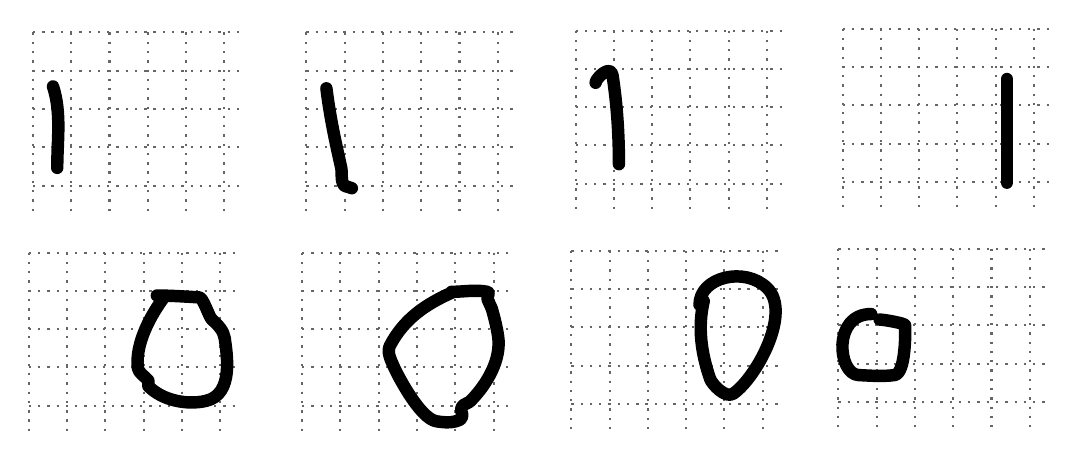
\begin{tikzpicture}[x=0.75pt,y=0.75pt,yscale=-1.5,xscale=1.5]
%uncomment if require: \path (0,479); %set diagram left start at 0, and has height of 479

%Shape: Grid [id:dp8017742479015741] 
\draw  [draw opacity=0][dash pattern={on 0.84pt off 2.51pt}] (86.7,177) -- (153.73,177) -- (153.73,234.28) -- (86.7,234.28) -- cycle ; \draw  [color={rgb, 255:red, 103; green, 101; blue, 101 }  ,draw opacity=1 ][dash pattern={on 0.84pt off 2.51pt}] (86.7,177) -- (86.7,234.28)(98.99,177) -- (98.99,234.28)(111.29,177) -- (111.29,234.28)(123.59,177) -- (123.59,234.28)(135.88,177) -- (135.88,234.28)(148.18,177) -- (148.18,234.28) ; \draw  [color={rgb, 255:red, 103; green, 101; blue, 101 }  ,draw opacity=1 ][dash pattern={on 0.84pt off 2.51pt}] (86.7,177) -- (153.73,177)(86.7,189.3) -- (153.73,189.3)(86.7,201.59) -- (153.73,201.59)(86.7,213.89) -- (153.73,213.89)(86.7,226.19) -- (153.73,226.19) ; \draw  [color={rgb, 255:red, 103; green, 101; blue, 101 }  ,draw opacity=1 ][dash pattern={on 0.84pt off 2.51pt}]  ;
%Shape: Free Drawing [id:dp8064467449652992] 
\draw  [line width=4.5] [line join = round][line cap = round] (93.14,194.35) .. controls (95.89,202.74) and (94.5,211.78) .. (94.5,220.5) ;
%Shape: Grid [id:dp7763004534165105] 
\draw  [draw opacity=0][dash pattern={on 0.84pt off 2.51pt}] (174.52,177) -- (241.56,177) -- (241.56,234.28) -- (174.52,234.28) -- cycle ; \draw  [color={rgb, 255:red, 103; green, 101; blue, 101 }  ,draw opacity=1 ][dash pattern={on 0.84pt off 2.51pt}] (174.52,177) -- (174.52,234.28)(186.82,177) -- (186.82,234.28)(199.11,177) -- (199.11,234.28)(211.41,177) -- (211.41,234.28)(223.71,177) -- (223.71,234.28)(236,177) -- (236,234.28) ; \draw  [color={rgb, 255:red, 103; green, 101; blue, 101 }  ,draw opacity=1 ][dash pattern={on 0.84pt off 2.51pt}] (174.52,177) -- (241.56,177)(174.52,189.3) -- (241.56,189.3)(174.52,201.59) -- (241.56,201.59)(174.52,213.89) -- (241.56,213.89)(174.52,226.19) -- (241.56,226.19) ; \draw  [color={rgb, 255:red, 103; green, 101; blue, 101 }  ,draw opacity=1 ][dash pattern={on 0.84pt off 2.51pt}]  ;
%Shape: Free Drawing [id:dp7728025162953451] 
\draw  [line width=4.5] [line join = round][line cap = round] (180.96,194.95) .. controls (182.01,203.62) and (183.82,212.14) .. (185.73,220.5) .. controls (186.13,222.26) and (185.49,224.25) .. (186.41,225.85) .. controls (187.02,226.91) and (188.2,226.22) .. (189.13,227.04) ;
%Shape: Grid [id:dp29771297583850953] 
\draw  [draw opacity=0][dash pattern={on 0.84pt off 2.51pt}] (260.98,176.41) -- (328.02,176.41) -- (328.02,233.69) -- (260.98,233.69) -- cycle ; \draw  [color={rgb, 255:red, 103; green, 101; blue, 101 }  ,draw opacity=1 ][dash pattern={on 0.84pt off 2.51pt}] (260.98,176.41) -- (260.98,233.69)(273.28,176.41) -- (273.28,233.69)(285.58,176.41) -- (285.58,233.69)(297.87,176.41) -- (297.87,233.69)(310.17,176.41) -- (310.17,233.69)(322.47,176.41) -- (322.47,233.69) ; \draw  [color={rgb, 255:red, 103; green, 101; blue, 101 }  ,draw opacity=1 ][dash pattern={on 0.84pt off 2.51pt}] (260.98,176.41) -- (328.02,176.41)(260.98,188.7) -- (328.02,188.7)(260.98,201) -- (328.02,201)(260.98,213.3) -- (328.02,213.3)(260.98,225.59) -- (328.02,225.59) ; \draw  [color={rgb, 255:red, 103; green, 101; blue, 101 }  ,draw opacity=1 ][dash pattern={on 0.84pt off 2.51pt}]  ;
%Shape: Free Drawing [id:dp08059093421743646] 
\draw  [line width=4.5] [line join = round][line cap = round] (267.43,193.17) .. controls (267.43,191.71) and (272.31,187.08) .. (272.87,190.79) .. controls (274.32,200.23) and (274.92,209.79) .. (274.92,219.31) ;
%Shape: Grid [id:dp45413993373677175] 
\draw  [draw opacity=0][dash pattern={on 0.84pt off 2.51pt}] (346.77,175.81) -- (413.8,175.81) -- (413.8,233.09) -- (346.77,233.09) -- cycle ; \draw  [color={rgb, 255:red, 103; green, 101; blue, 101 }  ,draw opacity=1 ][dash pattern={on 0.84pt off 2.51pt}] (346.77,175.81) -- (346.77,233.09)(359.06,175.81) -- (359.06,233.09)(371.36,175.81) -- (371.36,233.09)(383.65,175.81) -- (383.65,233.09)(395.95,175.81) -- (395.95,233.09)(408.25,175.81) -- (408.25,233.09) ; \draw  [color={rgb, 255:red, 103; green, 101; blue, 101 }  ,draw opacity=1 ][dash pattern={on 0.84pt off 2.51pt}] (346.77,175.81) -- (413.8,175.81)(346.77,188.11) -- (413.8,188.11)(346.77,200.41) -- (413.8,200.41)(346.77,212.7) -- (413.8,212.7)(346.77,225) -- (413.8,225) ; \draw  [color={rgb, 255:red, 103; green, 101; blue, 101 }  ,draw opacity=1 ][dash pattern={on 0.84pt off 2.51pt}]  ;
%Shape: Free Drawing [id:dp7154116232984749] 
\draw  [line width=4.5] [line join = round][line cap = round] (399.5,191.98) .. controls (399.5,203.07) and (399.5,214.16) .. (399.5,225.26) ;
%Shape: Grid [id:dp2704962527573529] 
\draw  [draw opacity=0][dash pattern={on 0.84pt off 2.51pt}] (85.34,247.72) -- (152.37,247.72) -- (152.37,305) -- (85.34,305) -- cycle ; \draw  [color={rgb, 255:red, 103; green, 101; blue, 101 }  ,draw opacity=1 ][dash pattern={on 0.84pt off 2.51pt}] (85.34,247.72) -- (85.34,305)(97.63,247.72) -- (97.63,305)(109.93,247.72) -- (109.93,305)(122.23,247.72) -- (122.23,305)(134.52,247.72) -- (134.52,305)(146.82,247.72) -- (146.82,305) ; \draw  [color={rgb, 255:red, 103; green, 101; blue, 101 }  ,draw opacity=1 ][dash pattern={on 0.84pt off 2.51pt}] (85.34,247.72) -- (152.37,247.72)(85.34,260.02) -- (152.37,260.02)(85.34,272.31) -- (152.37,272.31)(85.34,284.61) -- (152.37,284.61)(85.34,296.9) -- (152.37,296.9) ; \draw  [color={rgb, 255:red, 103; green, 101; blue, 101 }  ,draw opacity=1 ][dash pattern={on 0.84pt off 2.51pt}]  ;
%Shape: Grid [id:dp20012418254236608] 
\draw  [draw opacity=0][dash pattern={on 0.84pt off 2.51pt}] (173.16,247.72) -- (240.19,247.72) -- (240.19,305) -- (173.16,305) -- cycle ; \draw  [color={rgb, 255:red, 103; green, 101; blue, 101 }  ,draw opacity=1 ][dash pattern={on 0.84pt off 2.51pt}] (173.16,247.72) -- (173.16,305)(185.46,247.72) -- (185.46,305)(197.75,247.72) -- (197.75,305)(210.05,247.72) -- (210.05,305)(222.35,247.72) -- (222.35,305)(234.64,247.72) -- (234.64,305) ; \draw  [color={rgb, 255:red, 103; green, 101; blue, 101 }  ,draw opacity=1 ][dash pattern={on 0.84pt off 2.51pt}] (173.16,247.72) -- (240.19,247.72)(173.16,260.02) -- (240.19,260.02)(173.16,272.31) -- (240.19,272.31)(173.16,284.61) -- (240.19,284.61)(173.16,296.9) -- (240.19,296.9) ; \draw  [color={rgb, 255:red, 103; green, 101; blue, 101 }  ,draw opacity=1 ][dash pattern={on 0.84pt off 2.51pt}]  ;
%Shape: Grid [id:dp9881793507958303] 
\draw  [draw opacity=0][dash pattern={on 0.84pt off 2.51pt}] (259.62,247.12) -- (326.66,247.12) -- (326.66,304.41) -- (259.62,304.41) -- cycle ; \draw  [color={rgb, 255:red, 103; green, 101; blue, 101 }  ,draw opacity=1 ][dash pattern={on 0.84pt off 2.51pt}] (259.62,247.12) -- (259.62,304.41)(271.92,247.12) -- (271.92,304.41)(284.22,247.12) -- (284.22,304.41)(296.51,247.12) -- (296.51,304.41)(308.81,247.12) -- (308.81,304.41)(321.1,247.12) -- (321.1,304.41) ; \draw  [color={rgb, 255:red, 103; green, 101; blue, 101 }  ,draw opacity=1 ][dash pattern={on 0.84pt off 2.51pt}] (259.62,247.12) -- (326.66,247.12)(259.62,259.42) -- (326.66,259.42)(259.62,271.72) -- (326.66,271.72)(259.62,284.01) -- (326.66,284.01)(259.62,296.31) -- (326.66,296.31) ; \draw  [color={rgb, 255:red, 103; green, 101; blue, 101 }  ,draw opacity=1 ][dash pattern={on 0.84pt off 2.51pt}]  ;
%Shape: Grid [id:dp5786980285185035] 
\draw  [draw opacity=0][dash pattern={on 0.84pt off 2.51pt}] (345.4,246.53) -- (412.44,246.53) -- (412.44,303.81) -- (345.4,303.81) -- cycle ; \draw  [color={rgb, 255:red, 103; green, 101; blue, 101 }  ,draw opacity=1 ][dash pattern={on 0.84pt off 2.51pt}] (345.4,246.53) -- (345.4,303.81)(357.7,246.53) -- (357.7,303.81)(370,246.53) -- (370,303.81)(382.29,246.53) -- (382.29,303.81)(394.59,246.53) -- (394.59,303.81)(406.89,246.53) -- (406.89,303.81) ; \draw  [color={rgb, 255:red, 103; green, 101; blue, 101 }  ,draw opacity=1 ][dash pattern={on 0.84pt off 2.51pt}] (345.4,246.53) -- (412.44,246.53)(345.4,258.83) -- (412.44,258.83)(345.4,271.12) -- (412.44,271.12)(345.4,283.42) -- (412.44,283.42)(345.4,295.72) -- (412.44,295.72) ; \draw  [color={rgb, 255:red, 103; green, 101; blue, 101 }  ,draw opacity=1 ][dash pattern={on 0.84pt off 2.51pt}]  ;
%Shape: Free Drawing [id:dp07051563274345996] 
\draw  [line width=4.5] [line join = round][line cap = round] (129.22,261.51) .. controls (124.41,267.81) and (119.57,276.93) .. (120.37,284.68) .. controls (120.55,286.38) and (122.69,287.43) .. (123.78,288.84) .. controls (124.15,289.34) and (123.33,290.17) .. (123.78,290.63) .. controls (128.16,295.09) and (135.81,296.77) .. (142.16,295.38) .. controls (151.5,293.34) and (148.86,279.69) .. (148.29,275.18) .. controls (147.99,272.88) and (146.07,270.87) .. (144.2,269.23) .. controls (143.25,268.4) and (141.4,262.17) .. (140.12,262.1) .. controls (135.58,261.85) and (131.04,261.51) .. (126.5,261.51) ;
%Shape: Free Drawing [id:dp20550417919662056] 
\draw  [line width=4.5] [line join = round][line cap = round] (221.81,260.32) .. controls (212.92,264.2) and (205.93,268.96) .. (201.39,277.55) .. controls (200.23,279.74) and (201.79,282.42) .. (202.75,284.68) .. controls (203.32,286.02) and (210.86,301.12) .. (216.37,301.92) .. controls (218.38,302.21) and (220.56,302.48) .. (222.49,301.92) .. controls (226.66,300.71) and (223.27,299.09) .. (224.54,297.16) .. controls (225.1,296.3) and (226.52,296.13) .. (227.26,295.38) .. controls (232.62,289.92) and (237.22,281.99) .. (236.11,274.58) .. controls (235.66,271.58) and (234.91,268.61) .. (234.07,265.67) .. controls (233.77,264.63) and (232.97,263.74) .. (232.71,262.7) .. controls (232.51,261.92) and (233.59,260.5) .. (232.71,260.32) .. controls (228.95,259.55) and (224.99,260.32) .. (221.13,260.32) ;
%Shape: Free Drawing [id:dp981270324750338] 
\draw  [line width=4.5] [line join = round][line cap = round] (302.15,263.29) .. controls (300.22,271.72) and (301.32,279.89) .. (304.19,288.25) .. controls (304.77,289.93) and (309.16,294.76) .. (311.68,293) .. controls (319.13,287.8) and (330.45,266.92) .. (322.57,259.13) .. controls (315.4,252.04) and (300.79,255.57) .. (300.79,264.48) ;
%Shape: Free Drawing [id:dp5609590941584457] 
\draw  [line width=4.5] [line join = round][line cap = round] (355.93,267.45) .. controls (343.39,267.45) and (345.26,286.76) .. (351.85,287.06) .. controls (355.7,287.24) and (359.61,287.56) .. (363.42,287.06) .. controls (367.17,286.57) and (366.94,272.33) .. (366.82,271.02) .. controls (366.77,270.42) and (359.88,269.23) .. (358.65,269.23) ;




\end{tikzpicture}

    \caption{Sample from Ex~\ref{exl:real}~(c)}
    \label{fig:real-sample}
\end{figure}

\begin{figure}

\begin{subfigure}{\textwidth}
    \centering
    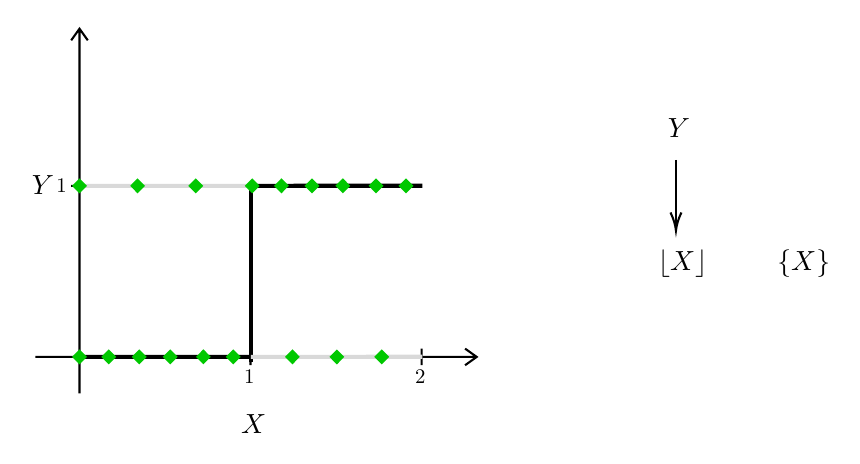
\begin{tikzpicture}[x=0.75pt,y=0.75pt,yscale=-0.8,xscale=0.8]
%uncomment if require: \path (0,300); %set diagram left start at 0, and has height of 300

%Shape: Axis 2D [id:dp15929656305777318] 
\draw  (84,230.66) -- (349.8,230.66)(110.58,33) -- (110.58,252.63) (342.8,225.66) -- (349.8,230.66) -- (342.8,235.66) (105.58,40) -- (110.58,33) -- (115.58,40) (213.58,225.66) -- (213.58,235.66)(316.58,225.66) -- (316.58,235.66)(105.58,127.66) -- (115.58,127.66) ;
\draw   (220.58,242.66) node[anchor=east, scale=0.75]{1} (323.58,242.66) node[anchor=east, scale=0.75]{2} (107.58,127.66) node[anchor=east, scale=0.75]{1} ;
%Straight Lines [id:da9513990505280441] 
\draw [line width=1.5]    (110.58,230.66) -- (213.8,230.63) ;
%Straight Lines [id:da8468292967898499] 
\draw [line width=1.5]    (213.8,127.63) -- (317.02,127.59) ;
%Straight Lines [id:da2700316228000621] 
\draw [line width=1.5]    (213.8,233.63) -- (213.8,127.63) ;
%Straight Lines [id:da9356502827423359] 
\draw [color={rgb, 255:red, 217; green, 217; blue, 217 }  ,draw opacity=1 ][line width=1.5]    (110.58,127.66) -- (213.8,127.63) ;
%Straight Lines [id:da07343551163457196] 
\draw [color={rgb, 255:red, 217; green, 217; blue, 217 }  ,draw opacity=1 ][line width=1.5]    (213.8,230.63) -- (317.02,230.59) ;
%Straight Lines [id:da10908447515776465] 
\draw    (469.8,112.03) -- (469.8,152.6) ;
\draw [shift={(469.8,154.6)}, rotate = 270] [color={rgb, 255:red, 0; green, 0; blue, 0 }  ][line width=0.75]    (10.93,-3.29) .. controls (6.95,-1.4) and (3.31,-0.3) .. (0,0) .. controls (3.31,0.3) and (6.95,1.4) .. (10.93,3.29)   ;
%Flowchart: Decision [id:dp2730919480254719] 
\draw  [color={rgb, 255:red, 0; green, 200; blue, 0 }  ,draw opacity=1 ][fill={rgb, 255:red, 0; green, 200; blue, 0 }  ,fill opacity=1 ] (203.19,226.99) -- (206.8,230.63) -- (203.19,234.26) -- (199.58,230.63) -- cycle ;
%Flowchart: Decision [id:dp11538103388031651] 
\draw  [color={rgb, 255:red, 0; green, 200; blue, 0 }  ,draw opacity=1 ][fill={rgb, 255:red, 0; green, 200; blue, 0 }  ,fill opacity=1 ] (185.19,226.99) -- (188.8,230.63) -- (185.19,234.26) -- (181.58,230.63) -- cycle ;
%Flowchart: Decision [id:dp5552720829266882] 
\draw  [color={rgb, 255:red, 0; green, 200; blue, 0 }  ,draw opacity=1 ][fill={rgb, 255:red, 0; green, 200; blue, 0 }  ,fill opacity=1 ] (165.19,226.99) -- (168.8,230.63) -- (165.19,234.26) -- (161.58,230.63) -- cycle ;
%Flowchart: Decision [id:dp3673189644014716] 
\draw  [color={rgb, 255:red, 0; green, 200; blue, 0 }  ,draw opacity=1 ][fill={rgb, 255:red, 0; green, 200; blue, 0 }  ,fill opacity=1 ] (146.58,227.01) -- (150.19,230.64) -- (146.58,234.28) -- (142.97,230.64) -- cycle ;
%Flowchart: Decision [id:dp5678180760919296] 
\draw  [color={rgb, 255:red, 0; green, 200; blue, 0 }  ,draw opacity=1 ][fill={rgb, 255:red, 0; green, 200; blue, 0 }  ,fill opacity=1 ] (128.19,226.99) -- (131.8,230.63) -- (128.19,234.26) -- (124.58,230.63) -- cycle ;
%Flowchart: Decision [id:dp9230338498592716] 
\draw  [color={rgb, 255:red, 0; green, 200; blue, 0 }  ,draw opacity=1 ][fill={rgb, 255:red, 0; green, 200; blue, 0 }  ,fill opacity=1 ] (110.58,227.03) -- (114.19,230.66) -- (110.58,234.3) -- (106.97,230.66) -- cycle ;
%Flowchart: Decision [id:dp862619117724202] 
\draw  [color={rgb, 255:red, 0; green, 200; blue, 0 }  ,draw opacity=1 ][fill={rgb, 255:red, 0; green, 200; blue, 0 }  ,fill opacity=1 ] (180.58,124.01) -- (184.19,127.64) -- (180.58,131.28) -- (176.97,127.64) -- cycle ;
%Flowchart: Decision [id:dp4358350481153632] 
\draw  [color={rgb, 255:red, 0; green, 200; blue, 0 }  ,draw opacity=1 ][fill={rgb, 255:red, 0; green, 200; blue, 0 }  ,fill opacity=1 ] (307.19,123.99) -- (310.8,127.63) -- (307.19,131.26) -- (303.58,127.63) -- cycle ;
%Flowchart: Decision [id:dp4275350413314525] 
\draw  [color={rgb, 255:red, 0; green, 200; blue, 0 }  ,draw opacity=1 ][fill={rgb, 255:red, 0; green, 200; blue, 0 }  ,fill opacity=1 ] (289.19,123.99) -- (292.8,127.63) -- (289.19,131.26) -- (285.58,127.63) -- cycle ;
%Flowchart: Decision [id:dp959527488455219] 
\draw  [color={rgb, 255:red, 0; green, 200; blue, 0 }  ,draw opacity=1 ][fill={rgb, 255:red, 0; green, 200; blue, 0 }  ,fill opacity=1 ] (269.19,123.99) -- (272.8,127.63) -- (269.19,131.26) -- (265.58,127.63) -- cycle ;
%Flowchart: Decision [id:dp22427101513476977] 
\draw  [color={rgb, 255:red, 0; green, 200; blue, 0 }  ,draw opacity=1 ][fill={rgb, 255:red, 0; green, 200; blue, 0 }  ,fill opacity=1 ] (250.58,124.01) -- (254.19,127.64) -- (250.58,131.28) -- (246.97,127.64) -- cycle ;
%Flowchart: Decision [id:dp3174155223827364] 
\draw  [color={rgb, 255:red, 0; green, 200; blue, 0 }  ,draw opacity=1 ][fill={rgb, 255:red, 0; green, 200; blue, 0 }  ,fill opacity=1 ] (232.19,123.99) -- (235.8,127.63) -- (232.19,131.26) -- (228.58,127.63) -- cycle ;
%Flowchart: Decision [id:dp007498027505505878] 
\draw  [color={rgb, 255:red, 0; green, 200; blue, 0 }  ,draw opacity=1 ][fill={rgb, 255:red, 0; green, 200; blue, 0 }  ,fill opacity=1 ] (214.58,124.03) -- (218.19,127.66) -- (214.58,131.3) -- (210.97,127.66) -- cycle ;
%Flowchart: Decision [id:dp7119492175609519] 
\draw  [color={rgb, 255:red, 0; green, 200; blue, 0 }  ,draw opacity=1 ][fill={rgb, 255:red, 0; green, 200; blue, 0 }  ,fill opacity=1 ] (292.58,227.01) -- (296.19,230.64) -- (292.58,234.28) -- (288.97,230.64) -- cycle ;
%Flowchart: Decision [id:dp5877233901346162] 
\draw  [color={rgb, 255:red, 0; green, 200; blue, 0 }  ,draw opacity=1 ][fill={rgb, 255:red, 0; green, 200; blue, 0 }  ,fill opacity=1 ] (145.58,124.01) -- (149.19,127.64) -- (145.58,131.28) -- (141.97,127.64) -- cycle ;
%Flowchart: Decision [id:dp7655491697593138] 
\draw  [color={rgb, 255:red, 0; green, 200; blue, 0 }  ,draw opacity=1 ][fill={rgb, 255:red, 0; green, 200; blue, 0 }  ,fill opacity=1 ] (265.58,227.01) -- (269.19,230.64) -- (265.58,234.28) -- (261.97,230.64) -- cycle ;
%Flowchart: Decision [id:dp9160492117736398] 
\draw  [color={rgb, 255:red, 0; green, 200; blue, 0 }  ,draw opacity=1 ][fill={rgb, 255:red, 0; green, 200; blue, 0 }  ,fill opacity=1 ] (110.58,124.03) -- (114.19,127.66) -- (110.58,131.3) -- (106.97,127.66) -- cycle ;
%Flowchart: Decision [id:dp7901791199984556] 
\draw  [color={rgb, 255:red, 0; green, 200; blue, 0 }  ,draw opacity=1 ][fill={rgb, 255:red, 0; green, 200; blue, 0 }  ,fill opacity=1 ] (238.8,226.99) -- (242.41,230.63) -- (238.8,234.26) -- (235.19,230.63) -- cycle ;

% Text Node
\draw (206,263.4) node [anchor=north west][inner sep=0.75pt]    {$X$};
% Text Node
\draw (80,119.4) node [anchor=north west][inner sep=0.75pt]    {$Y$};
% Text Node
\draw (463,85.4) node [anchor=north west][inner sep=0.75pt]    {$Y$};
% Text Node
\draw (457,164.4) node [anchor=north west][inner sep=0.75pt]    {$\lfloor X\rfloor $};
% Text Node
\draw (529,164.4) node [anchor=north west][inner sep=0.75pt]    {$\{X\}$};


\end{tikzpicture}

    \caption{Ex~\ref{exl:toy-a}}
    \label{fig:toy-a}
\end{subfigure}

\bigskip

\begin{subfigure}{\textwidth}
    \centering
    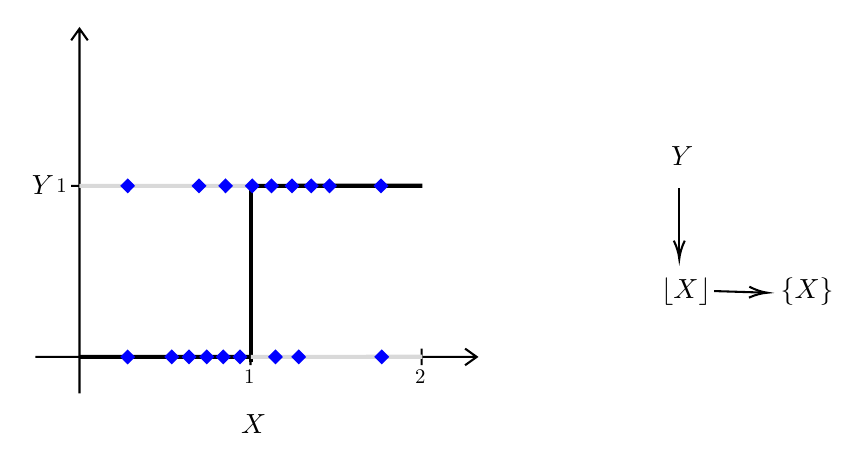
\begin{tikzpicture}[x=0.75pt,y=0.75pt,yscale=-0.8,xscale=0.8]
%uncomment if require: \path (0,300); %set diagram left start at 0, and has height of 300

%Straight Lines [id:da7814099327596118] 
\draw    (470.8,129) -- (470.8,169.58) ;
\draw [shift={(470.8,171.58)}, rotate = 270] [color={rgb, 255:red, 0; green, 0; blue, 0 }  ][line width=0.75]    (10.93,-3.29) .. controls (6.95,-1.4) and (3.31,-0.3) .. (0,0) .. controls (3.31,0.3) and (6.95,1.4) .. (10.93,3.29)   ;
%Straight Lines [id:da2463449188940814] 
\draw    (491.8,191) -- (521.8,191.94) ;
\draw [shift={(523.8,192)}, rotate = 181.79] [color={rgb, 255:red, 0; green, 0; blue, 0 }  ][line width=0.75]    (10.93,-3.29) .. controls (6.95,-1.4) and (3.31,-0.3) .. (0,0) .. controls (3.31,0.3) and (6.95,1.4) .. (10.93,3.29)   ;
%Shape: Axis 2D [id:dp8906483739192299] 
\draw  (83,230.66) -- (348.8,230.66)(109.58,33) -- (109.58,252.63) (341.8,225.66) -- (348.8,230.66) -- (341.8,235.66) (104.58,40) -- (109.58,33) -- (114.58,40) (212.58,225.66) -- (212.58,235.66)(315.58,225.66) -- (315.58,235.66)(104.58,127.66) -- (114.58,127.66) ;
\draw   (219.58,242.66) node[anchor=east, scale=0.75]{1} (322.58,242.66) node[anchor=east, scale=0.75]{2} (106.58,127.66) node[anchor=east, scale=0.75]{1} ;
%Straight Lines [id:da4015966345879818] 
\draw [line width=1.5]    (109.58,230.66) -- (212.8,230.63) ;
%Straight Lines [id:da34087071826352777] 
\draw [line width=1.5]    (212.8,127.63) -- (316.02,127.59) ;
%Straight Lines [id:da7757779318294376] 
\draw [line width=1.5]    (212.8,233.63) -- (212.8,127.63) ;
%Straight Lines [id:da7728976402558643] 
\draw [color={rgb, 255:red, 217; green, 217; blue, 217 }  ,draw opacity=1 ][line width=1.5]    (109.58,127.66) -- (212.8,127.63) ;
%Straight Lines [id:da8458194563907098] 
\draw [color={rgb, 255:red, 217; green, 217; blue, 217 }  ,draw opacity=1 ][line width=1.5]    (212.8,230.63) -- (316.02,230.59) ;
%Flowchart: Decision [id:dp031605134391225365] 
\draw  [color={rgb, 255:red, 0; green, 0; blue, 255 }  ,draw opacity=1 ][fill={rgb, 255:red, 0; green, 0; blue, 255 }  ,fill opacity=1 ] (206.19,226.99) -- (209.8,230.63) -- (206.19,234.26) -- (202.58,230.63) -- cycle ;
%Flowchart: Decision [id:dp8436663185315598] 
\draw  [color={rgb, 255:red, 0; green, 0; blue, 255 }  ,draw opacity=1 ][fill={rgb, 255:red, 0; green, 0; blue, 255 }  ,fill opacity=1 ] (196.19,226.99) -- (199.8,230.63) -- (196.19,234.26) -- (192.58,230.63) -- cycle ;
%Flowchart: Decision [id:dp7332568635958208] 
\draw  [color={rgb, 255:red, 0; green, 0; blue, 255 }  ,draw opacity=1 ][fill={rgb, 255:red, 0; green, 0; blue, 255 }  ,fill opacity=1 ] (186.19,226.99) -- (189.8,230.63) -- (186.19,234.26) -- (182.58,230.63) -- cycle ;
%Flowchart: Decision [id:dp17945566854317208] 
\draw  [color={rgb, 255:red, 0; green, 0; blue, 255 }  ,draw opacity=1 ][fill={rgb, 255:red, 0; green, 0; blue, 255 }  ,fill opacity=1 ] (175.58,227.01) -- (179.19,230.64) -- (175.58,234.28) -- (171.97,230.64) -- cycle ;
%Flowchart: Decision [id:dp04327280695327107] 
\draw  [color={rgb, 255:red, 0; green, 0; blue, 255 }  ,draw opacity=1 ][fill={rgb, 255:red, 0; green, 0; blue, 255 }  ,fill opacity=1 ] (165.19,226.99) -- (168.8,230.63) -- (165.19,234.26) -- (161.58,230.63) -- cycle ;
%Flowchart: Decision [id:dp28874218439414445] 
\draw  [color={rgb, 255:red, 0; green, 0; blue, 255 }  ,draw opacity=1 ][fill={rgb, 255:red, 0; green, 0; blue, 255 }  ,fill opacity=1 ] (138.58,227.03) -- (142.19,230.66) -- (138.58,234.3) -- (134.97,230.66) -- cycle ;
%Flowchart: Decision [id:dp7717740868946961] 
\draw  [color={rgb, 255:red, 0; green, 0; blue, 255 }  ,draw opacity=1 ][fill={rgb, 255:red, 0; green, 0; blue, 255 }  ,fill opacity=1 ] (197.58,124.01) -- (201.19,127.64) -- (197.58,131.28) -- (193.97,127.64) -- cycle ;
%Flowchart: Decision [id:dp10466642244648705] 
\draw  [color={rgb, 255:red, 0; green, 0; blue, 255 }  ,draw opacity=1 ][fill={rgb, 255:red, 0; green, 0; blue, 255 }  ,fill opacity=1 ] (291.19,123.99) -- (294.8,127.63) -- (291.19,131.26) -- (287.58,127.63) -- cycle ;
%Flowchart: Decision [id:dp37290865191432254] 
\draw  [color={rgb, 255:red, 0; green, 0; blue, 255 }  ,draw opacity=1 ][fill={rgb, 255:red, 0; green, 0; blue, 255 }  ,fill opacity=1 ] (260.19,123.99) -- (263.8,127.63) -- (260.19,131.26) -- (256.58,127.63) -- cycle ;
%Flowchart: Decision [id:dp04796258079840099] 
\draw  [color={rgb, 255:red, 0; green, 0; blue, 255 }  ,draw opacity=1 ][fill={rgb, 255:red, 0; green, 0; blue, 255 }  ,fill opacity=1 ] (249.19,123.99) -- (252.8,127.63) -- (249.19,131.26) -- (245.58,127.63) -- cycle ;
%Flowchart: Decision [id:dp559570534361439] 
\draw  [color={rgb, 255:red, 0; green, 0; blue, 255 }  ,draw opacity=1 ][fill={rgb, 255:red, 0; green, 0; blue, 255 }  ,fill opacity=1 ] (237.58,124.01) -- (241.19,127.64) -- (237.58,131.28) -- (233.97,127.64) -- cycle ;
%Flowchart: Decision [id:dp4613002487763067] 
\draw  [color={rgb, 255:red, 0; green, 0; blue, 255 }  ,draw opacity=1 ][fill={rgb, 255:red, 0; green, 0; blue, 255 }  ,fill opacity=1 ] (225.19,123.99) -- (228.8,127.63) -- (225.19,131.26) -- (221.58,127.63) -- cycle ;
%Flowchart: Decision [id:dp1797852326742293] 
\draw  [color={rgb, 255:red, 0; green, 0; blue, 255 }  ,draw opacity=1 ][fill={rgb, 255:red, 0; green, 0; blue, 255 }  ,fill opacity=1 ] (213.58,124.03) -- (217.19,127.66) -- (213.58,131.3) -- (209.97,127.66) -- cycle ;
%Flowchart: Decision [id:dp9224824552479813] 
\draw  [color={rgb, 255:red, 0; green, 0; blue, 255 }  ,draw opacity=1 ][fill={rgb, 255:red, 0; green, 0; blue, 255 }  ,fill opacity=1 ] (241.58,227.01) -- (245.19,230.64) -- (241.58,234.28) -- (237.97,230.64) -- cycle ;
%Flowchart: Decision [id:dp33095307210282066] 
\draw  [color={rgb, 255:red, 0; green, 0; blue, 255 }  ,draw opacity=1 ][fill={rgb, 255:red, 0; green, 0; blue, 255 }  ,fill opacity=1 ] (181.58,124.01) -- (185.19,127.64) -- (181.58,131.28) -- (177.97,127.64) -- cycle ;
%Flowchart: Decision [id:dp8130525838258988] 
\draw  [color={rgb, 255:red, 0; green, 0; blue, 255 }  ,draw opacity=1 ][fill={rgb, 255:red, 0; green, 0; blue, 255 }  ,fill opacity=1 ] (227.58,227.01) -- (231.19,230.64) -- (227.58,234.28) -- (223.97,230.64) -- cycle ;
%Flowchart: Decision [id:dp9623590050033171] 
\draw  [color={rgb, 255:red, 0; green, 0; blue, 255 }  ,draw opacity=1 ][fill={rgb, 255:red, 0; green, 0; blue, 255 }  ,fill opacity=1 ] (138.58,124.01) -- (142.19,127.64) -- (138.58,131.28) -- (134.97,127.64) -- cycle ;
%Flowchart: Decision [id:dp34685307680469024] 
\draw  [color={rgb, 255:red, 0; green, 0; blue, 255 }  ,draw opacity=1 ][fill={rgb, 255:red, 0; green, 0; blue, 255 }  ,fill opacity=1 ] (291.58,227.01) -- (295.19,230.64) -- (291.58,234.28) -- (287.97,230.64) -- cycle ;

% Text Node
\draw (464,102.37) node [anchor=north west][inner sep=0.75pt]    {$Y$};
% Text Node
\draw (458,181.37) node [anchor=north west][inner sep=0.75pt]    {$\lfloor X\rfloor $};
% Text Node
\draw (530,181.37) node [anchor=north west][inner sep=0.75pt]    {$\{X\}$};
% Text Node
\draw (205,263.4) node [anchor=north west][inner sep=0.75pt]    {$X$};
% Text Node
\draw (79,119.4) node [anchor=north west][inner sep=0.75pt]    {$Y$};


\end{tikzpicture}

    \caption{Ex~\ref{exl:toy-b}}
    \label{fig:toy-b}
\end{subfigure}

\bigskip

\begin{subfigure}{\textwidth}
    \centering
    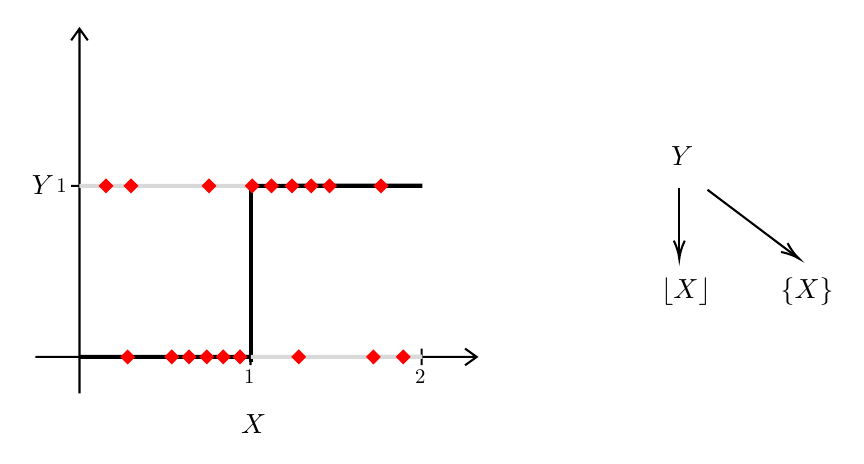
\begin{tikzpicture}[x=0.75pt,y=0.75pt,yscale=-0.8,xscale=0.8]
%uncomment if require: \path (0,300); %set diagram left start at 0, and has height of 300

%Straight Lines [id:da46729131782696465] 
\draw    (470.8,129) -- (470.8,169.58) ;
\draw [shift={(470.8,171.58)}, rotate = 270] [color={rgb, 255:red, 0; green, 0; blue, 0 }  ][line width=0.75]    (10.93,-3.29) .. controls (6.95,-1.4) and (3.31,-0.3) .. (0,0) .. controls (3.31,0.3) and (6.95,1.4) .. (10.93,3.29)   ;
%Straight Lines [id:da3163634970394127] 
\draw    (487.8,130) -- (541.2,170.2) ;
\draw [shift={(542.8,171.4)}, rotate = 216.97] [color={rgb, 255:red, 0; green, 0; blue, 0 }  ][line width=0.75]    (10.93,-3.29) .. controls (6.95,-1.4) and (3.31,-0.3) .. (0,0) .. controls (3.31,0.3) and (6.95,1.4) .. (10.93,3.29)   ;
%Shape: Axis 2D [id:dp09157075741024001] 
\draw  (83,230.66) -- (348.8,230.66)(109.58,33) -- (109.58,252.63) (341.8,225.66) -- (348.8,230.66) -- (341.8,235.66) (104.58,40) -- (109.58,33) -- (114.58,40) (212.58,225.66) -- (212.58,235.66)(315.58,225.66) -- (315.58,235.66)(104.58,127.66) -- (114.58,127.66) ;
\draw   (219.58,242.66) node[anchor=east, scale=0.75]{1} (322.58,242.66) node[anchor=east, scale=0.75]{2} (106.58,127.66) node[anchor=east, scale=0.75]{1} ;
%Straight Lines [id:da9594525928015434] 
\draw [line width=1.5]    (109.58,230.66) -- (212.8,230.63) ;
%Straight Lines [id:da8078087773819651] 
\draw [line width=1.5]    (212.8,127.63) -- (316.02,127.59) ;
%Straight Lines [id:da3764445013595581] 
\draw [line width=1.5]    (212.8,233.63) -- (212.8,127.63) ;
%Straight Lines [id:da21591384421539694] 
\draw [color={rgb, 255:red, 217; green, 217; blue, 217 }  ,draw opacity=1 ][line width=1.5]    (109.58,127.66) -- (212.8,127.63) ;
%Straight Lines [id:da5556202945981688] 
\draw [color={rgb, 255:red, 217; green, 217; blue, 217 }  ,draw opacity=1 ][line width=1.5]    (212.8,230.63) -- (316.02,230.59) ;
%Flowchart: Decision [id:dp7839916282263244] 
\draw  [color={rgb, 255:red, 255; green, 0; blue, 0 }  ,draw opacity=1 ][fill={rgb, 255:red, 255; green, 0; blue, 0 }  ,fill opacity=1 ] (206.19,226.99) -- (209.8,230.63) -- (206.19,234.26) -- (202.58,230.63) -- cycle ;
%Flowchart: Decision [id:dp6711485299143616] 
\draw  [color={rgb, 255:red, 255; green, 0; blue, 0 }  ,draw opacity=1 ][fill={rgb, 255:red, 255; green, 0; blue, 0 }  ,fill opacity=1 ] (196.19,226.99) -- (199.8,230.63) -- (196.19,234.26) -- (192.58,230.63) -- cycle ;
%Flowchart: Decision [id:dp7894615724105303] 
\draw  [color={rgb, 255:red, 255; green, 0; blue, 0 }  ,draw opacity=1 ][fill={rgb, 255:red, 255; green, 0; blue, 0 }  ,fill opacity=1 ] (186.19,226.99) -- (189.8,230.63) -- (186.19,234.26) -- (182.58,230.63) -- cycle ;
%Flowchart: Decision [id:dp7584526109922585] 
\draw  [color={rgb, 255:red, 255; green, 0; blue, 0 }  ,draw opacity=1 ][fill={rgb, 255:red, 255; green, 0; blue, 0 }  ,fill opacity=1 ] (175.58,227.01) -- (179.19,230.64) -- (175.58,234.28) -- (171.97,230.64) -- cycle ;
%Flowchart: Decision [id:dp8625449933978158] 
\draw  [color={rgb, 255:red, 255; green, 0; blue, 0 }  ,draw opacity=1 ][fill={rgb, 255:red, 255; green, 0; blue, 0 }  ,fill opacity=1 ] (165.19,226.99) -- (168.8,230.63) -- (165.19,234.26) -- (161.58,230.63) -- cycle ;
%Flowchart: Decision [id:dp19579639145005912] 
\draw  [color={rgb, 255:red, 255; green, 0; blue, 0 }  ,draw opacity=1 ][fill={rgb, 255:red, 255; green, 0; blue, 0 }  ,fill opacity=1 ] (138.58,227.03) -- (142.19,230.66) -- (138.58,234.3) -- (134.97,230.66) -- cycle ;
%Flowchart: Decision [id:dp3920435358532579] 
\draw  [color={rgb, 255:red, 255; green, 0; blue, 0 }  ,draw opacity=1 ][fill={rgb, 255:red, 255; green, 0; blue, 0 }  ,fill opacity=1 ] (187.58,124.01) -- (191.19,127.64) -- (187.58,131.28) -- (183.97,127.64) -- cycle ;
%Flowchart: Decision [id:dp6760724761124912] 
\draw  [color={rgb, 255:red, 255; green, 0; blue, 0 }  ,draw opacity=1 ][fill={rgb, 255:red, 255; green, 0; blue, 0 }  ,fill opacity=1 ] (291.19,123.99) -- (294.8,127.63) -- (291.19,131.26) -- (287.58,127.63) -- cycle ;
%Flowchart: Decision [id:dp2806401916742476] 
\draw  [color={rgb, 255:red, 255; green, 0; blue, 0 }  ,draw opacity=1 ][fill={rgb, 255:red, 255; green, 0; blue, 0 }  ,fill opacity=1 ] (260.19,123.99) -- (263.8,127.63) -- (260.19,131.26) -- (256.58,127.63) -- cycle ;
%Flowchart: Decision [id:dp2076148837465306] 
\draw  [color={rgb, 255:red, 255; green, 0; blue, 0 }  ,draw opacity=1 ][fill={rgb, 255:red, 255; green, 0; blue, 0 }  ,fill opacity=1 ] (249.19,123.99) -- (252.8,127.63) -- (249.19,131.26) -- (245.58,127.63) -- cycle ;
%Flowchart: Decision [id:dp8716986988905158] 
\draw  [color={rgb, 255:red, 255; green, 0; blue, 0 }  ,draw opacity=1 ][fill={rgb, 255:red, 255; green, 0; blue, 0 }  ,fill opacity=1 ] (237.58,124.01) -- (241.19,127.64) -- (237.58,131.28) -- (233.97,127.64) -- cycle ;
%Flowchart: Decision [id:dp4116451159943382] 
\draw  [color={rgb, 255:red, 255; green, 0; blue, 0 }  ,draw opacity=1 ][fill={rgb, 255:red, 255; green, 0; blue, 0 }  ,fill opacity=1 ] (225.19,123.99) -- (228.8,127.63) -- (225.19,131.26) -- (221.58,127.63) -- cycle ;
%Flowchart: Decision [id:dp5967455126851549] 
\draw  [color={rgb, 255:red, 255; green, 0; blue, 0 }  ,draw opacity=1 ][fill={rgb, 255:red, 255; green, 0; blue, 0 }  ,fill opacity=1 ] (213.58,124.03) -- (217.19,127.66) -- (213.58,131.3) -- (209.97,127.66) -- cycle ;
%Flowchart: Decision [id:dp1901681130027566] 
\draw  [color={rgb, 255:red, 255; green, 0; blue, 0 }  ,draw opacity=1 ][fill={rgb, 255:red, 255; green, 0; blue, 0 }  ,fill opacity=1 ] (286.58,227.01) -- (290.19,230.64) -- (286.58,234.28) -- (282.97,230.64) -- cycle ;
%Flowchart: Decision [id:dp639356618642068] 
\draw  [color={rgb, 255:red, 255; green, 0; blue, 0 }  ,draw opacity=1 ][fill={rgb, 255:red, 255; green, 0; blue, 0 }  ,fill opacity=1 ] (140.58,124.01) -- (144.19,127.64) -- (140.58,131.28) -- (136.97,127.64) -- cycle ;
%Flowchart: Decision [id:dp9189452492820236] 
\draw  [color={rgb, 255:red, 255; green, 0; blue, 0 }  ,draw opacity=1 ][fill={rgb, 255:red, 255; green, 0; blue, 0 }  ,fill opacity=1 ] (241.58,227.01) -- (245.19,230.64) -- (241.58,234.28) -- (237.97,230.64) -- cycle ;
%Flowchart: Decision [id:dp9044277291316816] 
\draw  [color={rgb, 255:red, 255; green, 0; blue, 0 }  ,draw opacity=1 ][fill={rgb, 255:red, 255; green, 0; blue, 0 }  ,fill opacity=1 ] (125.58,124.01) -- (129.19,127.64) -- (125.58,131.28) -- (121.97,127.64) -- cycle ;
%Flowchart: Decision [id:dp872931459829519] 
\draw  [color={rgb, 255:red, 255; green, 0; blue, 0 }  ,draw opacity=1 ][fill={rgb, 255:red, 255; green, 0; blue, 0 }  ,fill opacity=1 ] (304.58,227.01) -- (308.19,230.64) -- (304.58,234.28) -- (300.97,230.64) -- cycle ;

% Text Node
\draw (464,102.37) node [anchor=north west][inner sep=0.75pt]    {$Y$};
% Text Node
\draw (458,181.37) node [anchor=north west][inner sep=0.75pt]    {$\lfloor X\rfloor $};
% Text Node
\draw (530,181.37) node [anchor=north west][inner sep=0.75pt]    {$\{X\}$};
% Text Node
\draw (205,263.4) node [anchor=north west][inner sep=0.75pt]    {$X$};
% Text Node
\draw (79,119.4) node [anchor=north west][inner sep=0.75pt]    {$Y$};


\end{tikzpicture}

    \caption{Ex~\ref{exl:toy-c}}
    \label{fig:toy-c}
\end{subfigure}

\caption{Exs~\ref{exl:toy-a},~\ref{exl:toy-b},~\ref{exl:toy-c} -- (left) sample of joint distribution (right) causal diagram}

\label{fig:toy}

\end{figure}

\pagebreak
\section{Main result}
\label{sec:main}

In Def~\ref{dfn:inv-representation}, we defined what it meant for a representation -- a learning algorithm, as thought of as an estimate $Q(y\mid x)$ for the true posterior $\Prob{Y=y\mid X=x}$. In Def~\ref{dfn:inv-posterior}, we will define what it means for the true posterior $\Prob{Y=y\mid X=x}$ to be invariant.

\begin{dfn}[Invariant posterior]
    \label{dfn:inv-posterior}
    Let $\mathcal{X},\mathcal{Y}$ be sets and $X,Y$ are random quantities taking values in $\mathcal{X},\mathcal{Y}$; suppose we can factor $\mathcal{X}=\mathcal{X}_1\times\mathcal{X}_2$, writing each $X=(X_1,X_2)$. We say that the posterior $\Prob{Y\mid X}$ is $X_2$-invariant if $\Prob{Y\mid X_1, X_2}=\Prob{Y\mid X_1}$, i.e. $Y\ci X_2\mid X_1$. 
\end{dfn}

Note that Def~\ref{dfn:inv-posterior} is similar in spirit to Def~\ref{dfn:inv-stat-sxchen} -- both talk about the invariance of a probability distribution, rather than of a representation. However, Def~\ref{dfn:inv-posterior} speaks of invariance of the conditional distribution $\Prob{Y\mid X}$ while Def~\ref{dfn:inv-stat-sxchen} speaks of the invariance of the joint distribution $\Prob{X, Y}$ -- the former is more useful for supervised learning applications. We do, however have:

\begin{prop}[Def~\ref{dfn:inv-stat-sxchen} vs. Def~\ref{dfn:inv-posterior}]
    \label{prop:inv-stat-sxchen}
    Consider the set-up in Def~\ref{dfn:inv-stat-sxchen}; suppose we can factor $\mathcal{Z}=\mathcal{X}\times\mathcal{Y}$ so $Z=(X,Y)$, and that the action of $G$ can be decomposed onto this factorization $g(x, y)=(g(x), g(y))$ with all its stabilizers on $\mathcal{X}$ trivial and its action on $\mathcal{Y}$ trivial ($\mathrm{id}$). Further define $\mathcal{X}_1:=\mathcal{X}/G$ (the set of orbits) and $\mathcal{X}_2:=G$ -- by Lemma~\ref{lem:group}, there is a bijection $\phi:\mathcal{X}_1\times \mathcal{X}_2\simeq \mathcal{X}$, so we can define the random variables $(X_1, X_2)=\phi^{-1}(X)$ taking values in $\mathcal{X}_1$, $\mathcal{X}_2$.
    
    If $\Prob{Y\mid X}$ is $X_2$-invariant (Def~\ref{dfn:inv-posterior}) and $X$ is $G$-invariant (Def~\ref{dfn:inv-stat-sxchen}), then $Z$ is $G$-invariant (Def~\ref{dfn:inv-stat-sxchen}).
\end{prop}
\begin{proof}
    
    \begin{align*}
        & \Prob{Y\mid X}\text{ is }X_2-\text{invariant.} \\
        & \iff \Prob{Y\mid X_1, X_2}=\Prob{Y\mid X_1} \\
        & X\text{ is }G-\text{invariant.} \\ 
        & \iff \forall g, \, X =_d gX \\
        & \iff \forall x, g, \, \Prob{X=x} = \Prob{X = gx} \\
        & \iff \forall x, g, \, \Prob{(X_1, X_2)=\phi^{-1}(x)} = \Prob{(X_1, X_2)=\phi^{-1}(gx)} \\
        & \iff \forall x_1,x_2,x'_2, \, \Prob{X_1=x_1, X_2=x_2}=\Prob{X_1=x_1, X_2=x'_2} \\
        & \iff \Prob{X_1, X_2}=\Prob{X_1} \\
    \end{align*}
    \begin{align*}
        & Z\text{ is }G-\text{invariant.} \\ 
        & \iff \forall g, \, Z =_d gZ \\
        & \iff \forall g, \, (X, Y) =_d (gX, Y) \\
        & \iff \forall x, y, g, \, \Prob{X = x, Y = y} = \Prob{X = gx, Y = y} \\
        & \iff \forall x, y, g, \, \Prob{(X_1, X_2) = \phi^{-1}(x), Y = y} = \Prob{(X_1, X_2) = \phi^{-1}(gx), Y = y} \\
        & \iff \forall x_1, x_2, x'_2, y, \, \Prob{X_1=x_1, X_2=x_2, Y = y} = \Prob{X_1=x_1, X_2=x'_2, Y = y} \\
        & \iff \Prob{X_1, X_2, Y}=\Prob{X_1, Y}
    \end{align*}

    %$X$ is $G$-invariant $\iff$ $\forall g, \, X =_d gX$ $\iff$ $\forall x, g, \, \Prob{X=x} = \Prob{X = gx}$ $\iff$ $\forall x, g, \, \Prob{(X_1, X_2)=\phi^{-1}(x)} = \Prob{(X_1, X_2)=\phi^{-1}(gx)}$ $\iff$ $\forall x_1,x_2,x'_2, \, \Prob{X_1=x_1, X_2=x_2}=\Prob{X_1=x_1, X_2=x'_2}$ $\iff$ $\Prob{X_1, X_2}=\ProbP{X_1}$. 

    % $Z$ is $G$-invariant $\iff$ $\forall g, \, Z =_d gZ$ $\iff$ $\forall g, \, (X, Y) =_d (gX, Y)$ (since the action of $G$ on $\mathcal{Y}$ is trivial) $\iff$ $\forall x, y, g, \, \Prob{X = x, Y = y} = \Prob{X = gx, Y = y}$ $\iff$ $\forall x, y, g, \, \Prob{(X_1, X_2) = \phi^{-1}(x), Y = y} = \Prob{(X_1, X_2) = \phi^{-1}(gx), Y = y}$ $\iff$ $\forall x_1, x_2, x'_2, y, \, \Prob{X_1=x_1, X_2=x_2, Y = y} = \Prob{X_1=x_1, X_2=x'_2, Y = y}$ $\iff$ $\Prob{X_1, X_2, Y}=\Prob{X_1, Y}$.
    
    Suppose the hypotheses. Then:
    
    $\Prob{X_1, X_2, Y}= \Prob{Y\mid X_1, X_2}\Prob{X_1, X_2} = \Prob{Y\mid X_1}\Prob{X_1}=\Prob{X_1, Y}$.
    
    (This is the proof for discrete $\mathcal{Z}$ -- for the continuous case, one may suitably replace probability mass functions by probability density functions.)
\end{proof}

(This is in fact a correction to the paper \cite{sxchen} -- the paper itself states that Def~\ref{dfn:inv-stat-sxchen} means ``the probability of an image being a bird is [...] the same as the probability for a rotated image'', which as we discussed in Sec~\ref{sec:intro}, is incorrect -- in fact, this is Def~\ref{dfn:inv-posterior}, which is not equivalent. This is the reason we had to introduce Def~\ref{dfn:inv-posterior}, as it is what is relevant for supervised learning applications.)

We are finally ready to state our main result.

\begin{thm}[Condition for invariant learning to be suitable]
    \label{thm:main}
    In Framework~\ref{fw}, observe that $\Prob{Y\mid X}$ minimizes the risk among all distributions, and $\Prob{Y\mid X_1}$ minimizes the risk among all invariant distributions. We claim that for any $\varepsilon > 0$, $R(\Prob{Y\mid X_1}) - R(\Prob{Y\mid X}) < \varepsilon$ holds if (not necessarily only if) either:
    \begin{itemize}
        \item $\Prob{Y\mid X}$ is $X_2$-invariant in the sense of Def~\ref{dfn:inv-posterior}, in which case $R(\Prob{Y\mid X_1}) - R(\Prob{Y\mid X}) = 0$. 
        \item $\Ent{Y\mid X_1}<\varepsilon$.
    \end{itemize}
\end{thm}
\begin{proof}
    \begin{align*}
        & R(\Prob{Y\mid X})\\
        &= \E[X]{\Ent{\Prob{Y\mid X}, \Prob{Y\mid X}}} \\
        &= \E[x\sim X]{\sum_{y\in\mathcal{Y}}{\Prob{Y=y\mid X=x}\log\Prob{Y=y\mid X=x}}} \\ 
        &= \sum_{x,y\in\mathcal{X}, \mathcal{Y}}{\Prob{X=x}\Prob{Y=y\mid X=x}\log\Prob{Y=y\mid X=x}} \\ 
        &=\sum_{x,y\in\mathcal{X}, \mathcal{Y}}{\Prob{X=x,Y=y}\log\Prob{Y=y\mid X=x}} \\
        &= \Ent{Y\mid X} \\
        & R(\Prob{Y\mid X_1} \\
        &= \E[X]{\Ent{\Prob{Y\mid X}, \Prob{Y\mid X_1}}} \\
        &= \E[x\sim X]{\sum_{y\in \mathcal{Y}}{\Prob{Y=y\mid X=x}}\log\Prob{Y=y\mid X_1=x_1}} \\
    \end{align*}
    \begin{align*}
        &= \sum_{x,y\in\mathcal{X},\mathcal{Y}}{\Prob{X=x}\Prob{Y=y\mid X=x}\log\Prob{Y=y\mid X_1=x_1}} \\
        &= \sum_{x,y\in\mathcal{X},\mathcal{Y}}{\Prob{X=x,Y=y}\log\Prob{Y=y\mid X_1=x_1}} \\
        &= \sum_{x_1,x_2,y\in\mathcal{X}_1,\mathcal{X}_2,\mathcal{Y}}{\Prob{X_2=x_2\mid X_1=x_1, Y=y}\Prob{X_1=x_1,Y=y}\log\Prob{Y=y\mid X_1=x_1}} \\
        &= \sum_{x_1, y\in\mathcal{X}_1,\mathcal{Y}}{\left[\Prob{X_1=x_1, Y=y}\log\Prob{Y=y\mid X_1=x_1}\sum_{x_2\in\mathcal{X}_2}{\Prob{X_2=x_2\mid X_1=x_1, Y=y}}\right]} \\ 
        &= \sum_{x_1, y\in\mathcal{X}_1,\mathcal{Y}}{\left[\Prob{X_1=x_1, Y=y}\log\Prob{Y=y\mid X_1=x_1}\cdot 1\right]}\\
        &= \Ent{Y\mid X_1}
    \end{align*}
    
    If we have invariant posterior, then simply $\Prob{Y\mid X_1}=\Prob{Y\mid X}$. If $\Ent{Y\mid X_1}<\varepsilon$, observe that by Lemma~\ref{lem:condition}, $\Ent{Y\mid X} = \Ent{Y\mid X_1, X_2} \le \Ent{Y\mid X_1} < \varepsilon$. Thus $R(\Prob{Y\mid X_1})-R(\Prob{Y\mid X})= \Ent{Y\mid X_1} - \Ent{Y\mid X}<\varepsilon$.
\end{proof}

Thus in these situations, the ``best invariant distribution'' does no more than $\varepsilon$ worse than the ``best distribution'' -- our previous observation about invariance still making sense in the absence of an invariant posterior is therefore reduced to an information-theoretic result. The following corollary is a more direct answer to the question ``When is invariant learning effective?''.

\begin{cor}
    \label{cor:main}
    Let $Q$ and $Q'$ be the minimum-loss estimator and the minimum-loss invariant estimator for $P(Y\mid X)$ respectively. Then for any $\varepsilon>0$, $\E{L(Q')-L(Q)}<\varepsilon$ if (not necessarily only if) either:
    \begin{itemize}
        \item $\Prob{Y\mid X}$ is $X_2$-invariant in the sense of Def~\ref{dfn:inv-posterior}, in which case $R(\Prob{Y\mid X_1}) - R(\Prob{Y\mid X}) = 0$. 
        \item $\Ent{Y\mid X_1}<\varepsilon$.
    \end{itemize}
\end{cor}

\pagebreak
\section{Conclusion}
\label{sec:concl}

We began our investigation with the following observation: even when some ``nuisance factor'' $X_2$ provides non-redundant information about the label $Y$ in a supervised learning application, it is sometimes safe to ignore this factor (i.e. use a learning algorithm that was invariant to this factor), as it was in Fig~\ref{fig:real-sample-0}. Certainly, the loss would be greater than if the factor was incorporated -- but still low, so we could hope for a bound on it. Intuitively, we imagined that the reason that we could do so in Fig~\ref{fig:real-sample-0} was that the other factors $X_1$, namely the ``shape'' provides ``sufficient information'' on $Y$, so in some sense the information propagated from $X_1$ to $Y$ ``dominates'' that propagated from $X_2$ to $Y$. Crucially, we saw in our analysis of Ex~\ref{exl:toy-c} that this domination happens \emph{independently} of the amount of information provided by $X_2$ on $Y$. 

Our main result, Thm~\ref{thm:main} formalizes this observation as an information theoretic result: specifically, we demonstrate that the expected loss $R(Q)$ for the distribution $P(Y\mid X)$ is precisely the conditional entropy $H(Y\mid X)$, and for the invariant distribution $P(Y\mid X_1)$ is precisely the conditional entropy $H(Y\mid X_1)$, which is a measure of the uncertainty that remains in $Y$ after knowing $X_1$.

This result can be interpreted in the light of our motivating questions. 

For applications to fair machine learning, Thm~\ref{thm:main} says that the conditional mutual information $I(Y;X_2\mid X_1)=H(Y\mid X_1)-H(Y\mid X_1, X_2)$ becomes precisely the bound on the increased risk from learning invariant to sensitive characteristics $X_2$.

\begin{exl}[6 and 9 problem in Framework~\ref{fw}]
    \label{exl:69}
    Let $\mathcal{Y}=\{0, 1\}$ and $\mathcal{X}=\{x:\R^2\to\{0,1\}\}$ be the set of images; define $\mathcal{X}_2=\{T_U:\mathcal{X}\to\mathcal{X}:x\mapsto\lambda i. x(U^{-1}i)\mid U\in SO(2)\} \cong SO(2)$ to be the group of rotations acting on $\mathcal{X}$; define $\mathcal{X}_1=\mathcal{X}/\mathcal{X}_2$ to be the quotient by the group action (i.e. the orbits under rotation). By Lemma~\ref{lem:group}, there is a bijection $\phi:\mathcal{X}_1\times \mathcal{X}_2\to \mathcal{X}$ given by $\phi(O, T_v)=T_v\xi(O)$ where $\xi(O)$ is some representative in $O$; then $\phi^{-1}:x\mapsto ([x], T_{\theta(x)})$ where $T_{\theta(x)}\in\mathcal{X}_2$ is such that $T_{\theta(x)}\xi([x])=x$, which exists as $x$ is in the same orbit as $\xi([x])$. Composing this with the isomorphism $\mathcal{X}_2\cong SO(2)$ (given by $T_U\mapsto U$), we have $x\mapsto([x],\theta(x))$. Thus the decomposition $\mathcal{X}_1\times\mathcal{X}_2$ decomposes an image into its orbit under rotations (its ``shape'') and its angle from some representative element in its orbit (its ``angle'').
\end{exl} 

Ex~\ref{exl:69} formulates the 6 and 9 problem in the language of Framework~\ref{fw} -- in it, the posterior is not invariant: the angle $\theta(x)$ provides information on the label even knowing $[x]$, because a 6 and a 9 may be contained in the same orbit. And here invariant learning is not effective -- but we don't expect it to be anyway, because $H(Y\mid X_1)$ is large; we still have very little certainty on what the label is after knowing the orbit, leaving ``room'' for $X_2$ to take away this uncertainty. 

Our work is only some preliminary set-up for serious research into the problem of invariant learning in scenarios without invariant posteriors, which as we discussed in Sec~\ref{sec:intro} has many important implications. 

\begin{figure}
    \centering
    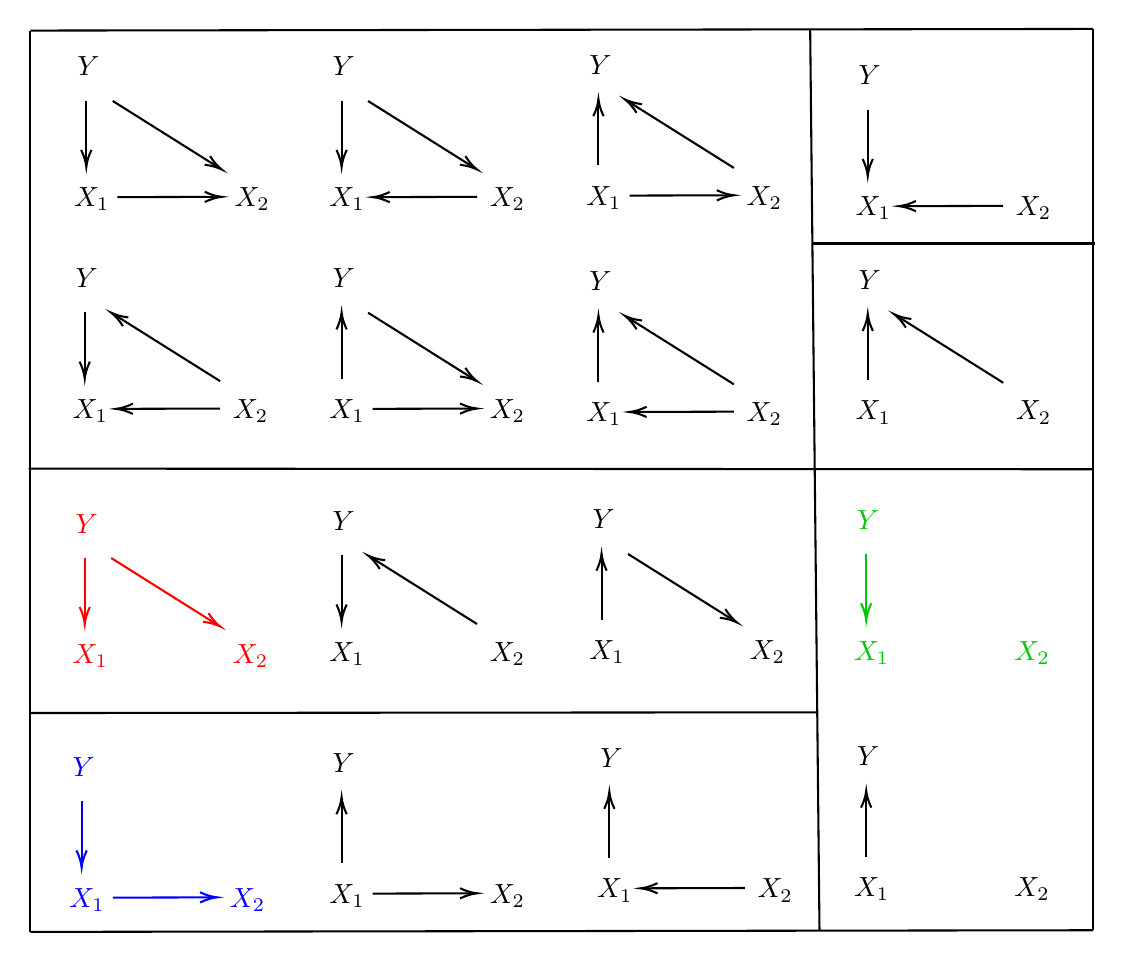
\begin{tikzpicture}[x=0.75pt,y=0.75pt,yscale=-0.75,xscale=0.75]
%uncomment if require: \path (0,1196); %set diagram left start at 0, and has height of 1196

%Straight Lines [id:da3737571818181842] 
\draw    (109.8,102.05) -- (109.8,142.63) ;
\draw [shift={(109.8,144.63)}, rotate = 270] [color={rgb, 255:red, 0; green, 0; blue, 0 }  ][line width=0.75]    (10.93,-3.29) .. controls (6.95,-1.4) and (3.31,-0.3) .. (0,0) .. controls (3.31,0.3) and (6.95,1.4) .. (10.93,3.29)   ;
%Straight Lines [id:da12363516406728814] 
\draw    (126.8,102.25) -- (195.11,145.19) ;
\draw [shift={(196.8,146.25)}, rotate = 212.15] [color={rgb, 255:red, 0; green, 0; blue, 0 }  ][line width=0.75]    (10.93,-3.29) .. controls (6.95,-1.4) and (3.31,-0.3) .. (0,0) .. controls (3.31,0.3) and (6.95,1.4) .. (10.93,3.29)   ;
%Straight Lines [id:da4016683557259253] 
\draw    (129.8,164.02) -- (194.8,163.83) ;
\draw [shift={(196.8,163.82)}, rotate = 179.83] [color={rgb, 255:red, 0; green, 0; blue, 0 }  ][line width=0.75]    (10.93,-3.29) .. controls (6.95,-1.4) and (3.31,-0.3) .. (0,0) .. controls (3.31,0.3) and (6.95,1.4) .. (10.93,3.29)   ;
%Straight Lines [id:da13979440957606548] 
\draw    (273.8,102.05) -- (273.8,142.63) ;
\draw [shift={(273.8,144.63)}, rotate = 270] [color={rgb, 255:red, 0; green, 0; blue, 0 }  ][line width=0.75]    (10.93,-3.29) .. controls (6.95,-1.4) and (3.31,-0.3) .. (0,0) .. controls (3.31,0.3) and (6.95,1.4) .. (10.93,3.29)   ;
%Straight Lines [id:da22702492120087414] 
\draw    (290.8,102.25) -- (359.11,145.19) ;
\draw [shift={(360.8,146.25)}, rotate = 212.15] [color={rgb, 255:red, 0; green, 0; blue, 0 }  ][line width=0.75]    (10.93,-3.29) .. controls (6.95,-1.4) and (3.31,-0.3) .. (0,0) .. controls (3.31,0.3) and (6.95,1.4) .. (10.93,3.29)   ;
%Straight Lines [id:da9841493229157976] 
\draw    (295.8,164.02) -- (360.8,163.82) ;
\draw [shift={(293.8,164.02)}, rotate = 359.83] [color={rgb, 255:red, 0; green, 0; blue, 0 }  ][line width=0.75]    (10.93,-3.29) .. controls (6.95,-1.4) and (3.31,-0.3) .. (0,0) .. controls (3.31,0.3) and (6.95,1.4) .. (10.93,3.29)   ;
%Straight Lines [id:da9924559937229132] 
\draw    (108.8,238.05) -- (108.8,278.63) ;
\draw [shift={(108.8,280.63)}, rotate = 270] [color={rgb, 255:red, 0; green, 0; blue, 0 }  ][line width=0.75]    (10.93,-3.29) .. controls (6.95,-1.4) and (3.31,-0.3) .. (0,0) .. controls (3.31,0.3) and (6.95,1.4) .. (10.93,3.29)   ;
%Straight Lines [id:da6768355425490677] 
\draw    (127.49,239.31) -- (195.8,282.25) ;
\draw [shift={(125.8,238.25)}, rotate = 32.15] [color={rgb, 255:red, 0; green, 0; blue, 0 }  ][line width=0.75]    (10.93,-3.29) .. controls (6.95,-1.4) and (3.31,-0.3) .. (0,0) .. controls (3.31,0.3) and (6.95,1.4) .. (10.93,3.29)   ;
%Straight Lines [id:da2071038961010725] 
\draw    (130.8,300.02) -- (195.8,299.82) ;
\draw [shift={(128.8,300.02)}, rotate = 359.83] [color={rgb, 255:red, 0; green, 0; blue, 0 }  ][line width=0.75]    (10.93,-3.29) .. controls (6.95,-1.4) and (3.31,-0.3) .. (0,0) .. controls (3.31,0.3) and (6.95,1.4) .. (10.93,3.29)   ;
%Straight Lines [id:da26722839420446753] 
\draw    (273.8,240.05) -- (273.8,280.63) ;
\draw [shift={(273.8,238.05)}, rotate = 90] [color={rgb, 255:red, 0; green, 0; blue, 0 }  ][line width=0.75]    (10.93,-3.29) .. controls (6.95,-1.4) and (3.31,-0.3) .. (0,0) .. controls (3.31,0.3) and (6.95,1.4) .. (10.93,3.29)   ;
%Straight Lines [id:da2755756022709992] 
\draw    (290.8,238.25) -- (359.11,281.19) ;
\draw [shift={(360.8,282.25)}, rotate = 212.15] [color={rgb, 255:red, 0; green, 0; blue, 0 }  ][line width=0.75]    (10.93,-3.29) .. controls (6.95,-1.4) and (3.31,-0.3) .. (0,0) .. controls (3.31,0.3) and (6.95,1.4) .. (10.93,3.29)   ;
%Straight Lines [id:da44976239734144907] 
\draw    (293.8,300.02) -- (358.8,299.83) ;
\draw [shift={(360.8,299.82)}, rotate = 179.83] [color={rgb, 255:red, 0; green, 0; blue, 0 }  ][line width=0.75]    (10.93,-3.29) .. controls (6.95,-1.4) and (3.31,-0.3) .. (0,0) .. controls (3.31,0.3) and (6.95,1.4) .. (10.93,3.29)   ;
%Straight Lines [id:da258977938558949] 
\draw    (438.8,103.05) -- (438.8,143.63) ;
\draw [shift={(438.8,101.05)}, rotate = 90] [color={rgb, 255:red, 0; green, 0; blue, 0 }  ][line width=0.75]    (10.93,-3.29) .. controls (6.95,-1.4) and (3.31,-0.3) .. (0,0) .. controls (3.31,0.3) and (6.95,1.4) .. (10.93,3.29)   ;
%Straight Lines [id:da087304581755838] 
\draw    (457.49,102.31) -- (525.8,145.25) ;
\draw [shift={(455.8,101.25)}, rotate = 32.15] [color={rgb, 255:red, 0; green, 0; blue, 0 }  ][line width=0.75]    (10.93,-3.29) .. controls (6.95,-1.4) and (3.31,-0.3) .. (0,0) .. controls (3.31,0.3) and (6.95,1.4) .. (10.93,3.29)   ;
%Straight Lines [id:da8613469044592399] 
\draw    (458.8,163.02) -- (523.8,162.83) ;
\draw [shift={(525.8,162.82)}, rotate = 179.83] [color={rgb, 255:red, 0; green, 0; blue, 0 }  ][line width=0.75]    (10.93,-3.29) .. controls (6.95,-1.4) and (3.31,-0.3) .. (0,0) .. controls (3.31,0.3) and (6.95,1.4) .. (10.93,3.29)   ;
%Straight Lines [id:da194364380318234] 
\draw    (438.8,242.05) -- (438.8,282.63) ;
\draw [shift={(438.8,240.05)}, rotate = 90] [color={rgb, 255:red, 0; green, 0; blue, 0 }  ][line width=0.75]    (10.93,-3.29) .. controls (6.95,-1.4) and (3.31,-0.3) .. (0,0) .. controls (3.31,0.3) and (6.95,1.4) .. (10.93,3.29)   ;
%Straight Lines [id:da5998872733134424] 
\draw    (457.49,241.31) -- (525.8,284.25) ;
\draw [shift={(455.8,240.25)}, rotate = 32.15] [color={rgb, 255:red, 0; green, 0; blue, 0 }  ][line width=0.75]    (10.93,-3.29) .. controls (6.95,-1.4) and (3.31,-0.3) .. (0,0) .. controls (3.31,0.3) and (6.95,1.4) .. (10.93,3.29)   ;
%Straight Lines [id:da10829433236098396] 
\draw    (460.8,302.02) -- (525.8,301.82) ;
\draw [shift={(458.8,302.02)}, rotate = 359.83] [color={rgb, 255:red, 0; green, 0; blue, 0 }  ][line width=0.75]    (10.93,-3.29) .. controls (6.95,-1.4) and (3.31,-0.3) .. (0,0) .. controls (3.31,0.3) and (6.95,1.4) .. (10.93,3.29)   ;
%Straight Lines [id:da08633400243561717] 
\draw [color={rgb, 255:red, 255; green, 0; blue, 0 }  ,draw opacity=1 ][fill={rgb, 255:red, 255; green, 0; blue, 0 }  ,fill opacity=1 ]   (108.8,395.65) -- (108.8,436.23) ;
\draw [shift={(108.8,438.23)}, rotate = 270] [color={rgb, 255:red, 255; green, 0; blue, 0 }  ,draw opacity=1 ][line width=0.75]    (10.93,-3.29) .. controls (6.95,-1.4) and (3.31,-0.3) .. (0,0) .. controls (3.31,0.3) and (6.95,1.4) .. (10.93,3.29)   ;
%Straight Lines [id:da14078609582582602] 
\draw [color={rgb, 255:red, 255; green, 0; blue, 0 }  ,draw opacity=1 ][fill={rgb, 255:red, 255; green, 0; blue, 0 }  ,fill opacity=1 ]   (125.8,395.85) -- (194.11,438.79) ;
\draw [shift={(195.8,439.85)}, rotate = 212.15] [color={rgb, 255:red, 255; green, 0; blue, 0 }  ,draw opacity=1 ][line width=0.75]    (10.93,-3.29) .. controls (6.95,-1.4) and (3.31,-0.3) .. (0,0) .. controls (3.31,0.3) and (6.95,1.4) .. (10.93,3.29)   ;
%Straight Lines [id:da17413565112347396] 
\draw    (273.8,394.05) -- (273.8,434.63) ;
\draw [shift={(273.8,436.63)}, rotate = 270] [color={rgb, 255:red, 0; green, 0; blue, 0 }  ][line width=0.75]    (10.93,-3.29) .. controls (6.95,-1.4) and (3.31,-0.3) .. (0,0) .. controls (3.31,0.3) and (6.95,1.4) .. (10.93,3.29)   ;
%Straight Lines [id:da6555200232339404] 
\draw    (292.49,395.31) -- (360.8,438.25) ;
\draw [shift={(290.8,394.25)}, rotate = 32.15] [color={rgb, 255:red, 0; green, 0; blue, 0 }  ][line width=0.75]    (10.93,-3.29) .. controls (6.95,-1.4) and (3.31,-0.3) .. (0,0) .. controls (3.31,0.3) and (6.95,1.4) .. (10.93,3.29)   ;
%Straight Lines [id:da7146044042109168] 
\draw    (440.8,395.05) -- (440.8,435.63) ;
\draw [shift={(440.8,393.05)}, rotate = 90] [color={rgb, 255:red, 0; green, 0; blue, 0 }  ][line width=0.75]    (10.93,-3.29) .. controls (6.95,-1.4) and (3.31,-0.3) .. (0,0) .. controls (3.31,0.3) and (6.95,1.4) .. (10.93,3.29)   ;
%Straight Lines [id:da5409264586826019] 
\draw    (457.8,393.25) -- (526.11,436.19) ;
\draw [shift={(527.8,437.25)}, rotate = 212.15] [color={rgb, 255:red, 0; green, 0; blue, 0 }  ][line width=0.75]    (10.93,-3.29) .. controls (6.95,-1.4) and (3.31,-0.3) .. (0,0) .. controls (3.31,0.3) and (6.95,1.4) .. (10.93,3.29)   ;
%Straight Lines [id:da23185239239309863] 
\draw    (72.8,338.42) -- (756.8,338.82) ;
%Straight Lines [id:da05961507981524283] 
\draw [color={rgb, 255:red, 0; green, 0; blue, 255 }  ,draw opacity=1 ][fill={rgb, 255:red, 0; green, 0; blue, 255 }  ,fill opacity=1 ]   (106.8,552.05) -- (106.8,592.63) ;
\draw [shift={(106.8,594.63)}, rotate = 270] [color={rgb, 255:red, 0; green, 0; blue, 255 }  ,draw opacity=1 ][line width=0.75]    (10.93,-3.29) .. controls (6.95,-1.4) and (3.31,-0.3) .. (0,0) .. controls (3.31,0.3) and (6.95,1.4) .. (10.93,3.29)   ;
%Straight Lines [id:da22314027893365873] 
\draw [color={rgb, 255:red, 0; green, 0; blue, 255 }  ,draw opacity=1 ][fill={rgb, 255:red, 0; green, 0; blue, 255 }  ,fill opacity=1 ]   (126.8,614.02) -- (191.8,613.83) ;
\draw [shift={(193.8,613.82)}, rotate = 179.83] [color={rgb, 255:red, 0; green, 0; blue, 255 }  ,draw opacity=1 ][line width=0.75]    (10.93,-3.29) .. controls (6.95,-1.4) and (3.31,-0.3) .. (0,0) .. controls (3.31,0.3) and (6.95,1.4) .. (10.93,3.29)   ;
%Straight Lines [id:da9186969757185328] 
\draw    (273.8,551.45) -- (273.8,592.03) ;
\draw [shift={(273.8,549.45)}, rotate = 90] [color={rgb, 255:red, 0; green, 0; blue, 0 }  ][line width=0.75]    (10.93,-3.29) .. controls (6.95,-1.4) and (3.31,-0.3) .. (0,0) .. controls (3.31,0.3) and (6.95,1.4) .. (10.93,3.29)   ;
%Straight Lines [id:da3953971002080736] 
\draw    (293.8,611.42) -- (358.8,611.23) ;
\draw [shift={(360.8,611.22)}, rotate = 179.83] [color={rgb, 255:red, 0; green, 0; blue, 0 }  ][line width=0.75]    (10.93,-3.29) .. controls (6.95,-1.4) and (3.31,-0.3) .. (0,0) .. controls (3.31,0.3) and (6.95,1.4) .. (10.93,3.29)   ;
%Straight Lines [id:da5490613008317458] 
\draw    (445.8,548.05) -- (445.8,588.63) ;
\draw [shift={(445.8,546.05)}, rotate = 90] [color={rgb, 255:red, 0; green, 0; blue, 0 }  ][line width=0.75]    (10.93,-3.29) .. controls (6.95,-1.4) and (3.31,-0.3) .. (0,0) .. controls (3.31,0.3) and (6.95,1.4) .. (10.93,3.29)   ;
%Straight Lines [id:da9077981531340531] 
\draw    (467.8,608.02) -- (532.8,607.82) ;
\draw [shift={(465.8,608.02)}, rotate = 359.83] [color={rgb, 255:red, 0; green, 0; blue, 0 }  ][line width=0.75]    (10.93,-3.29) .. controls (6.95,-1.4) and (3.31,-0.3) .. (0,0) .. controls (3.31,0.3) and (6.95,1.4) .. (10.93,3.29)   ;
%Straight Lines [id:da09681400807035945] 
\draw    (611.8,107.85) -- (611.8,148.43) ;
\draw [shift={(611.8,150.43)}, rotate = 270] [color={rgb, 255:red, 0; green, 0; blue, 0 }  ][line width=0.75]    (10.93,-3.29) .. controls (6.95,-1.4) and (3.31,-0.3) .. (0,0) .. controls (3.31,0.3) and (6.95,1.4) .. (10.93,3.29)   ;
%Straight Lines [id:da1546249903127026] 
\draw    (633.8,169.82) -- (698.8,169.62) ;
\draw [shift={(631.8,169.82)}, rotate = 359.83] [color={rgb, 255:red, 0; green, 0; blue, 0 }  ][line width=0.75]    (10.93,-3.29) .. controls (6.95,-1.4) and (3.31,-0.3) .. (0,0) .. controls (3.31,0.3) and (6.95,1.4) .. (10.93,3.29)   ;
%Straight Lines [id:da1446952319748649] 
\draw    (611.8,241.05) -- (611.8,281.63) ;
\draw [shift={(611.8,239.05)}, rotate = 90] [color={rgb, 255:red, 0; green, 0; blue, 0 }  ][line width=0.75]    (10.93,-3.29) .. controls (6.95,-1.4) and (3.31,-0.3) .. (0,0) .. controls (3.31,0.3) and (6.95,1.4) .. (10.93,3.29)   ;
%Straight Lines [id:da0175675608880288] 
\draw    (630.49,240.31) -- (698.8,283.25) ;
\draw [shift={(628.8,239.25)}, rotate = 32.15] [color={rgb, 255:red, 0; green, 0; blue, 0 }  ][line width=0.75]    (10.93,-3.29) .. controls (6.95,-1.4) and (3.31,-0.3) .. (0,0) .. controls (3.31,0.3) and (6.95,1.4) .. (10.93,3.29)   ;
%Straight Lines [id:da7728749191826159] 
\draw [color={rgb, 255:red, 0; green, 200; blue, 0 }  ,draw opacity=1 ][fill={rgb, 255:red, 0; green, 200; blue, 0 }  ,fill opacity=1 ]   (610.8,393.25) -- (610.8,433.83) ;
\draw [shift={(610.8,435.83)}, rotate = 270] [color={rgb, 255:red, 0; green, 200; blue, 0 }  ,draw opacity=1 ][line width=0.75]    (10.93,-3.29) .. controls (6.95,-1.4) and (3.31,-0.3) .. (0,0) .. controls (3.31,0.3) and (6.95,1.4) .. (10.93,3.29)   ;
%Straight Lines [id:da7844152258995551] 
\draw    (610.8,547.25) -- (610.8,587.83) ;
\draw [shift={(610.8,545.25)}, rotate = 90] [color={rgb, 255:red, 0; green, 0; blue, 0 }  ][line width=0.75]    (10.93,-3.29) .. controls (6.95,-1.4) and (3.31,-0.3) .. (0,0) .. controls (3.31,0.3) and (6.95,1.4) .. (10.93,3.29)   ;
%Straight Lines [id:da23519247995534265] 
\draw    (73.8,495.42) -- (578.61,494.96) ;
%Straight Lines [id:da7326143142124661] 
\draw    (574.8,55.82) -- (580.8,635.43) ;
%Straight Lines [id:da472841715824615] 
\draw    (575.8,193.82) -- (757.8,193.82) ;
%Straight Lines [id:da45380400421965716] 
\draw    (73.8,57.02) -- (756.61,55.96) ;
%Straight Lines [id:da22076004711772246] 
\draw    (73.8,636.02) -- (756.61,634.96) ;
%Straight Lines [id:da4411113148877692] 
\draw    (756.61,55.96) -- (756.61,634.96) ;
%Straight Lines [id:da6312398068118072] 
\draw    (73.8,57.02) -- (73.8,636.02) ;

% Text Node
\draw (100,156.03) node [anchor=north west][inner sep=0.75pt]    {$X_{1}$};
% Text Node
\draw (102,72.03) node [anchor=north west][inner sep=0.75pt]    {$Y$};
% Text Node
\draw (203,156.03) node [anchor=north west][inner sep=0.75pt]    {$X_{2}$};
% Text Node
\draw (264,156.03) node [anchor=north west][inner sep=0.75pt]    {$X_{1}$};
% Text Node
\draw (266,72.03) node [anchor=north west][inner sep=0.75pt]    {$Y$};
% Text Node
\draw (367,156.03) node [anchor=north west][inner sep=0.75pt]    {$X_{2}$};
% Text Node
\draw (99,292.03) node [anchor=north west][inner sep=0.75pt]    {$X_{1}$};
% Text Node
\draw (101,208.03) node [anchor=north west][inner sep=0.75pt]    {$Y$};
% Text Node
\draw (202,292.03) node [anchor=north west][inner sep=0.75pt]    {$X_{2}$};
% Text Node
\draw (264,292.03) node [anchor=north west][inner sep=0.75pt]    {$X_{1}$};
% Text Node
\draw (266,208.03) node [anchor=north west][inner sep=0.75pt]    {$Y$};
% Text Node
\draw (367,292.03) node [anchor=north west][inner sep=0.75pt]    {$X_{2}$};
% Text Node
\draw (429,155.03) node [anchor=north west][inner sep=0.75pt]    {$X_{1}$};
% Text Node
\draw (431,71.03) node [anchor=north west][inner sep=0.75pt]    {$Y$};
% Text Node
\draw (532,155.03) node [anchor=north west][inner sep=0.75pt]    {$X_{2}$};
% Text Node
\draw (429,294.03) node [anchor=north west][inner sep=0.75pt]    {$X_{1}$};
% Text Node
\draw (431,210.03) node [anchor=north west][inner sep=0.75pt]    {$Y$};
% Text Node
\draw (532,294.03) node [anchor=north west][inner sep=0.75pt]    {$X_{2}$};
% Text Node
\draw (99,449.63) node [anchor=north west][inner sep=0.75pt]  [color={rgb, 255:red, 255; green, 0; blue, 0 }  ,opacity=1 ]  {$X_{1}$};
% Text Node
\draw (101,365.63) node [anchor=north west][inner sep=0.75pt]  [color={rgb, 255:red, 255; green, 0; blue, 0 }  ,opacity=1 ]  {$Y$};
% Text Node
\draw (202,449.63) node [anchor=north west][inner sep=0.75pt]  [color={rgb, 255:red, 255; green, 0; blue, 0 }  ,opacity=1 ]  {$X_{2}$};
% Text Node
\draw (264,448.03) node [anchor=north west][inner sep=0.75pt]    {$X_{1}$};
% Text Node
\draw (266,364.03) node [anchor=north west][inner sep=0.75pt]    {$Y$};
% Text Node
\draw (367,448.03) node [anchor=north west][inner sep=0.75pt]    {$X_{2}$};
% Text Node
\draw (431,447.03) node [anchor=north west][inner sep=0.75pt]    {$X_{1}$};
% Text Node
\draw (433,363.03) node [anchor=north west][inner sep=0.75pt]    {$Y$};
% Text Node
\draw (534,447.03) node [anchor=north west][inner sep=0.75pt]    {$X_{2}$};
% Text Node
\draw (97,606.03) node [anchor=north west][inner sep=0.75pt]  [color={rgb, 255:red, 0; green, 0; blue, 255 }  ,opacity=1 ]  {$X_{1}$};
% Text Node
\draw (99,522.03) node [anchor=north west][inner sep=0.75pt]  [color={rgb, 255:red, 0; green, 0; blue, 255 }  ,opacity=1 ]  {$Y$};
% Text Node
\draw (200,606.03) node [anchor=north west][inner sep=0.75pt]  [color={rgb, 255:red, 0; green, 0; blue, 255 }  ,opacity=1 ]  {$X_{2}$};
% Text Node
\draw (264,603.43) node [anchor=north west][inner sep=0.75pt]    {$X_{1}$};
% Text Node
\draw (266,519.43) node [anchor=north west][inner sep=0.75pt]    {$Y$};
% Text Node
\draw (367,603.43) node [anchor=north west][inner sep=0.75pt]    {$X_{2}$};
% Text Node
\draw (436,600.03) node [anchor=north west][inner sep=0.75pt]    {$X_{1}$};
% Text Node
\draw (438,516.03) node [anchor=north west][inner sep=0.75pt]    {$Y$};
% Text Node
\draw (539,600.03) node [anchor=north west][inner sep=0.75pt]    {$X_{2}$};
% Text Node
\draw (602,161.83) node [anchor=north west][inner sep=0.75pt]    {$X_{1}$};
% Text Node
\draw (604,77.83) node [anchor=north west][inner sep=0.75pt]    {$Y$};
% Text Node
\draw (705,161.83) node [anchor=north west][inner sep=0.75pt]    {$X_{2}$};
% Text Node
\draw (602,293.03) node [anchor=north west][inner sep=0.75pt]    {$X_{1}$};
% Text Node
\draw (604,209.02) node [anchor=north west][inner sep=0.75pt]    {$Y$};
% Text Node
\draw (705,293.03) node [anchor=north west][inner sep=0.75pt]    {$X_{2}$};
% Text Node
\draw (601,447.23) node [anchor=north west][inner sep=0.75pt]  [color={rgb, 255:red, 0; green, 200; blue, 0 }  ,opacity=1 ]  {$X_{1}$};
% Text Node
\draw (603,363.23) node [anchor=north west][inner sep=0.75pt]  [color={rgb, 255:red, 0; green, 200; blue, 0 }  ,opacity=1 ]  {$Y$};
% Text Node
\draw (704,447.23) node [anchor=north west][inner sep=0.75pt]  [color={rgb, 255:red, 0; green, 200; blue, 0 }  ,opacity=1 ]  {$X_{2}$};
% Text Node
\draw (601,599.23) node [anchor=north west][inner sep=0.75pt]    {$X_{1}$};
% Text Node
\draw (603,515.23) node [anchor=north west][inner sep=0.75pt]    {$Y$};
% Text Node
\draw (704,599.23) node [anchor=north west][inner sep=0.75pt]    {$X_{2}$};


\end{tikzpicture}

    \caption{All possible causal diagrams that contain an edge between $Y$ and $X_1$; the boxes are Markov equivalence classes; the causal structures for Exs~\ref{exl:toy-a},~\ref{exl:toy-b},~\ref{exl:toy-c} are in green, blue and red respectively.}
    \label{fig:exls}
\end{figure}

\begin{figure}
    \centering
    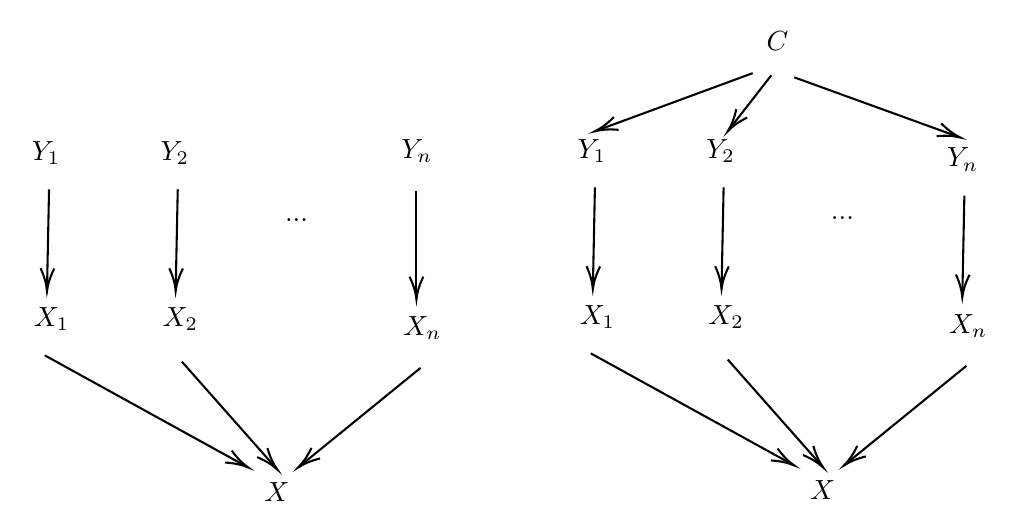
\begin{tikzpicture}[x=0.75pt,y=0.75pt,yscale=-1,xscale=1]
%uncomment if require: \path (0,300); %set diagram left start at 0, and has height of 300

%Straight Lines [id:da269330412207331] 
\draw    (424.8,123.81) -- (423.84,170.81) ;
\draw [shift={(423.8,172.81)}, rotate = 271.17] [color={rgb, 255:red, 0; green, 0; blue, 0 }  ][line width=0.75]    (10.93,-3.29) .. controls (6.95,-1.4) and (3.31,-0.3) .. (0,0) .. controls (3.31,0.3) and (6.95,1.4) .. (10.93,3.29)   ;
%Straight Lines [id:da20163910952116182] 
\draw    (486.8,123.81) -- (485.84,170.81) ;
\draw [shift={(485.8,172.81)}, rotate = 271.17] [color={rgb, 255:red, 0; green, 0; blue, 0 }  ][line width=0.75]    (10.93,-3.29) .. controls (6.95,-1.4) and (3.31,-0.3) .. (0,0) .. controls (3.31,0.3) and (6.95,1.4) .. (10.93,3.29)   ;
%Straight Lines [id:da3153413719669911] 
\draw    (602.8,127.81) -- (601.84,174.81) ;
\draw [shift={(601.8,176.81)}, rotate = 271.17] [color={rgb, 255:red, 0; green, 0; blue, 0 }  ][line width=0.75]    (10.93,-3.29) .. controls (6.95,-1.4) and (3.31,-0.3) .. (0,0) .. controls (3.31,0.3) and (6.95,1.4) .. (10.93,3.29)   ;
%Straight Lines [id:da3819029344613025] 
\draw    (422.8,203.81) -- (519.05,256.85) ;
\draw [shift={(520.8,257.81)}, rotate = 208.86] [color={rgb, 255:red, 0; green, 0; blue, 0 }  ][line width=0.75]    (10.93,-3.29) .. controls (6.95,-1.4) and (3.31,-0.3) .. (0,0) .. controls (3.31,0.3) and (6.95,1.4) .. (10.93,3.29)   ;
%Straight Lines [id:da9852908613435107] 
\draw    (488.8,206.81) -- (533.47,257.31) ;
\draw [shift={(534.8,258.81)}, rotate = 228.5] [color={rgb, 255:red, 0; green, 0; blue, 0 }  ][line width=0.75]    (10.93,-3.29) .. controls (6.95,-1.4) and (3.31,-0.3) .. (0,0) .. controls (3.31,0.3) and (6.95,1.4) .. (10.93,3.29)   ;
%Straight Lines [id:da8061644228162519] 
\draw    (603.8,209.81) -- (546.35,256.55) ;
\draw [shift={(544.8,257.81)}, rotate = 320.87] [color={rgb, 255:red, 0; green, 0; blue, 0 }  ][line width=0.75]    (10.93,-3.29) .. controls (6.95,-1.4) and (3.31,-0.3) .. (0,0) .. controls (3.31,0.3) and (6.95,1.4) .. (10.93,3.29)   ;
%Straight Lines [id:da7760456749060423] 
\draw    (500.8,68.81) -- (426.68,96.12) ;
\draw [shift={(424.8,96.81)}, rotate = 339.78] [color={rgb, 255:red, 0; green, 0; blue, 0 }  ][line width=0.75]    (10.93,-3.29) .. controls (6.95,-1.4) and (3.31,-0.3) .. (0,0) .. controls (3.31,0.3) and (6.95,1.4) .. (10.93,3.29)   ;
%Straight Lines [id:da05795133399036745] 
\draw    (509.8,69.81) -- (490.03,95.23) ;
\draw [shift={(488.8,96.81)}, rotate = 307.87] [color={rgb, 255:red, 0; green, 0; blue, 0 }  ][line width=0.75]    (10.93,-3.29) .. controls (6.95,-1.4) and (3.31,-0.3) .. (0,0) .. controls (3.31,0.3) and (6.95,1.4) .. (10.93,3.29)   ;
%Straight Lines [id:da06836865562937366] 
\draw    (520.8,70.81) -- (598.92,99.13) ;
\draw [shift={(600.8,99.81)}, rotate = 199.93] [color={rgb, 255:red, 0; green, 0; blue, 0 }  ][line width=0.75]    (10.93,-3.29) .. controls (6.95,-1.4) and (3.31,-0.3) .. (0,0) .. controls (3.31,0.3) and (6.95,1.4) .. (10.93,3.29)   ;
%Straight Lines [id:da9926207953521895] 
\draw    (161.8,124.81) -- (160.84,171.81) ;
\draw [shift={(160.8,173.81)}, rotate = 271.17] [color={rgb, 255:red, 0; green, 0; blue, 0 }  ][line width=0.75]    (10.93,-3.29) .. controls (6.95,-1.4) and (3.31,-0.3) .. (0,0) .. controls (3.31,0.3) and (6.95,1.4) .. (10.93,3.29)   ;
%Straight Lines [id:da8568136901286545] 
\draw    (223.8,124.81) -- (222.84,171.81) ;
\draw [shift={(222.8,173.81)}, rotate = 271.17] [color={rgb, 255:red, 0; green, 0; blue, 0 }  ][line width=0.75]    (10.93,-3.29) .. controls (6.95,-1.4) and (3.31,-0.3) .. (0,0) .. controls (3.31,0.3) and (6.95,1.4) .. (10.93,3.29)   ;
%Straight Lines [id:da740570735568955] 
\draw    (338.8,125.42) -- (338.8,175.81) ;
\draw [shift={(338.8,177.81)}, rotate = 270] [color={rgb, 255:red, 0; green, 0; blue, 0 }  ][line width=0.75]    (10.93,-3.29) .. controls (6.95,-1.4) and (3.31,-0.3) .. (0,0) .. controls (3.31,0.3) and (6.95,1.4) .. (10.93,3.29)   ;
%Straight Lines [id:da07973497484566927] 
\draw    (159.8,204.81) -- (256.05,257.85) ;
\draw [shift={(257.8,258.81)}, rotate = 208.86] [color={rgb, 255:red, 0; green, 0; blue, 0 }  ][line width=0.75]    (10.93,-3.29) .. controls (6.95,-1.4) and (3.31,-0.3) .. (0,0) .. controls (3.31,0.3) and (6.95,1.4) .. (10.93,3.29)   ;
%Straight Lines [id:da9415378984840401] 
\draw    (225.8,207.81) -- (270.47,258.31) ;
\draw [shift={(271.8,259.81)}, rotate = 228.5] [color={rgb, 255:red, 0; green, 0; blue, 0 }  ][line width=0.75]    (10.93,-3.29) .. controls (6.95,-1.4) and (3.31,-0.3) .. (0,0) .. controls (3.31,0.3) and (6.95,1.4) .. (10.93,3.29)   ;
%Straight Lines [id:da15035733725472755] 
\draw    (340.8,210.81) -- (283.35,257.55) ;
\draw [shift={(281.8,258.81)}, rotate = 320.87] [color={rgb, 255:red, 0; green, 0; blue, 0 }  ][line width=0.75]    (10.93,-3.29) .. controls (6.95,-1.4) and (3.31,-0.3) .. (0,0) .. controls (3.31,0.3) and (6.95,1.4) .. (10.93,3.29)   ;

% Text Node
\draw (415,99.4) node [anchor=north west][inner sep=0.75pt]    {$Y_{1}$};
% Text Node
\draw (416,179.4) node [anchor=north west][inner sep=0.75pt]    {$X_{1}$};
% Text Node
\draw (477,99.4) node [anchor=north west][inner sep=0.75pt]    {$Y_{2}$};
% Text Node
\draw (478,179.4) node [anchor=north west][inner sep=0.75pt]    {$X_{2}$};
% Text Node
\draw (537,136.4) node [anchor=north west][inner sep=0.75pt]    {$...$};
% Text Node
\draw (593,103.4) node [anchor=north west][inner sep=0.75pt]    {$Y_{n}$};
% Text Node
\draw (594,183.4) node [anchor=north west][inner sep=0.75pt]    {$X_{n}$};
% Text Node
\draw (527,263.4) node [anchor=north west][inner sep=0.75pt]    {$X$};
% Text Node
\draw (506,47.4) node [anchor=north west][inner sep=0.75pt]    {$C$};
% Text Node
\draw (152,100.4) node [anchor=north west][inner sep=0.75pt]    {$Y_{1}$};
% Text Node
\draw (153,180.4) node [anchor=north west][inner sep=0.75pt]    {$X_{1}$};
% Text Node
\draw (214,100.4) node [anchor=north west][inner sep=0.75pt]    {$Y_{2}$};
% Text Node
\draw (215,180.4) node [anchor=north west][inner sep=0.75pt]    {$X_{2}$};
% Text Node
\draw (274,137.4) node [anchor=north west][inner sep=0.75pt]    {$...$};
% Text Node
\draw (330,99.4) node [anchor=north west][inner sep=0.75pt]    {$Y_{n}$};
% Text Node
\draw (331,184.4) node [anchor=north west][inner sep=0.75pt]    {$X_{n}$};
% Text Node
\draw (264,264.4) node [anchor=north west][inner sep=0.75pt]    {$X$};


\end{tikzpicture}

    \caption{(left) Equivariant posterior (right) Non-equivariant posterior due to confounding variable, i.e. common cause introducing correlation}
    \label{fig:equivariant}
\end{figure}

We now outline several directions for further research in this area.

\begin{enumerate}

    \item Our result is specifically for the cross-entropy loss -- while this is a natural loss function to take (especially for our motivating examples), and it is a rather beautiful result that the condition on this loss being bounded is also an information-theoretic one, we may be interested in other loss functions, and these would be bounded by corresponding measures of conditional uncertainty other than the conditional entropy. 
    
    For example, I would conjecture that the corresponding bound for the mean-squared-error loss (for continuous $Y$) would be the conditional variance $\mathrm{Var}(Y\mid X_1)$. It would be of interest to see a general result, perhaps in the light of empirical risk minimization theory.
    
    \item Our work stands in analogy to the results in \cite{sxchen}, in the sense that the two sufficient cases in Thm~\ref{thm:main} are analogous to the results in \cite{sxchen} for ``exact invariance'' and ``approximate invariance''; however, this is a rather vague analogy, in that our second case is unrelated to approximate invariance (while our first case is related to exact invariance by Prop~\ref{prop:inv-stat-sxchen}).
    
    More generally, Thm~\ref{thm:main} only provides \emph{sufficient} conditions for invariant learning to be suitable. The converse problem is significantly harder, as the loss from invariant learning may also be bounded if $P(Y\mid X_1)$ is ``approximately equal'' in distribution to $P(Y\mid X)$. In \cite{sxchen}, ``approximately equal in distribution'' is defined in terms of the Wasserstein metric. 
    
    \item In Sec~\ref{sec:intro}, we briefly hinted that invariant learning is thought to be suitable precisely in the anti-causal direction. While the second sufficient case in Thm~\ref{thm:main} does not make any direct reference to the causal structure, this is relevant to the converse problem. Fig~\ref{fig:exls} is an exhaustive list of all the relevant possible causal structures between variables $Y, X_1, X_2$ -- we ought to formally investigate and justify which causal structures is invariant learning rational for.
    
    More generally, one may consider similar problems for generalized learning algorithms on arbitrary causal diagrams -- this would be relevant to generalizing our work to \emph{equivariant} learning. We have not provided a formal definition of equivariance beyond the basic definition in Def~\ref{dfn:inv-det-group}; however, I would suggest that the causal diagram for an ``equivariant posterior'' would look like Fig~\ref{fig:equivariant}~(left). 
    
    \item While Thm~\ref{thm:main} provides conditions for invariant learning to be no worse than (or rather ``no more than $\varepsilon$ worse than'') non-invariant learning, it does not give reasons as to why one \emph{should} adopt invariant learning in the first place -- what makes it \emph{better}, even in the second sufficient case where the loss is in fact greater. This is in contrast to the work of \cite{sxchen}, which demonstrates that an estimator learned through invariant learning has lower variance, by providing a decomposition of the covariance of the non-invariantly learned estimator into the covariance of the invariantly learned estimator and another positive-definite matrix. 
    
    Our representation $Q(y\mid x)$ is a random function, so we conjecture that the \emph{covariance kernel} of the non-invariantly learned $Q(y\mid x)$ into the covariance kernel of the invariantly learned $Q(y\mid x)$ and another positive-definite kernel. Studying the covariance kernel of $Q(y\mid x)$ would also help us prove Corollary~\ref{cor:main}, perhaps through an application of the multidimensional Chebyshev inequality. 
    
    \item In contrast to algorithms that learn invariantly to a given set of symmetries, there are various algorithms in the literature that aim to learn the group of symmetries from the dataset itself, e.g. \cite{benton, cubuk, wilk}. This is a goal rather similar to ours -- from our perspective, a group $G$ is a subgroup of the symmetry group for a task if $H(Y\mid X_1)-H(Y\mid X)$ is small (where $X_1$ are the $G$-orbits), and we can estimate $H(Y\mid X_1)$ from the data\footnote{Estimating entropy from data is not, in general, a simple task, but there are various estimators available, e.g. \cite{entropy1, entropy2, entropy3}}.
    
    We may then ask two relevant questions thereof: (1) Would an algorithm like in \cite{benton, cubuk, wilk} discover an invariance in the second sufficient case, i.e. when the posterior is not truly invariant? (2) Can we use this to produce an algorithm that \emph{learns} the symmetries of a task -- rather than simply check it? -- i.e. an algorithm to find a factorization of $\mathcal{X}$ that minimizes $H(Y\mid X_1)$.
\end{enumerate}

\section{Acknowledgements}

I would like to thank my supervisor Prof Jeroen Lamb and PhD student Victoria Klein for their valuable comments on earlier drafts. 

And I would like to thank Rev Srikesh Maadhapuzhi Swaminathan Iyer Hegde -- for \emph{nothing}. For all the pressure I've put on him, what I've gotten in return? Nothing! Doesn't even rise to greet me. 

\pagebreak
\printbibliography[heading=bibintoc, title={References}]

\end{document}